% Options for packages loaded elsewhere
\PassOptionsToPackage{unicode}{hyperref}
\PassOptionsToPackage{hyphens}{url}
\PassOptionsToPackage{dvipsnames,svgnames,x11names}{xcolor}
%
\documentclass[
  letterpaper,
  DIV=11,
  numbers=noendperiod]{scrreprt}

\usepackage{amsmath,amssymb}
\usepackage{iftex}
\ifPDFTeX
  \usepackage[T1]{fontenc}
  \usepackage[utf8]{inputenc}
  \usepackage{textcomp} % provide euro and other symbols
\else % if luatex or xetex
  \usepackage{unicode-math}
  \defaultfontfeatures{Scale=MatchLowercase}
  \defaultfontfeatures[\rmfamily]{Ligatures=TeX,Scale=1}
\fi
\usepackage{lmodern}
\ifPDFTeX\else  
    % xetex/luatex font selection
\fi
% Use upquote if available, for straight quotes in verbatim environments
\IfFileExists{upquote.sty}{\usepackage{upquote}}{}
\IfFileExists{microtype.sty}{% use microtype if available
  \usepackage[]{microtype}
  \UseMicrotypeSet[protrusion]{basicmath} % disable protrusion for tt fonts
}{}
\makeatletter
\@ifundefined{KOMAClassName}{% if non-KOMA class
  \IfFileExists{parskip.sty}{%
    \usepackage{parskip}
  }{% else
    \setlength{\parindent}{0pt}
    \setlength{\parskip}{6pt plus 2pt minus 1pt}}
}{% if KOMA class
  \KOMAoptions{parskip=half}}
\makeatother
\usepackage{xcolor}
\usepackage{soul}
\setlength{\emergencystretch}{3em} % prevent overfull lines
\setcounter{secnumdepth}{5}
% Make \paragraph and \subparagraph free-standing
\ifx\paragraph\undefined\else
  \let\oldparagraph\paragraph
  \renewcommand{\paragraph}[1]{\oldparagraph{#1}\mbox{}}
\fi
\ifx\subparagraph\undefined\else
  \let\oldsubparagraph\subparagraph
  \renewcommand{\subparagraph}[1]{\oldsubparagraph{#1}\mbox{}}
\fi

\usepackage{color}
\usepackage{fancyvrb}
\newcommand{\VerbBar}{|}
\newcommand{\VERB}{\Verb[commandchars=\\\{\}]}
\DefineVerbatimEnvironment{Highlighting}{Verbatim}{commandchars=\\\{\}}
% Add ',fontsize=\small' for more characters per line
\usepackage{framed}
\definecolor{shadecolor}{RGB}{241,243,245}
\newenvironment{Shaded}{\begin{snugshade}}{\end{snugshade}}
\newcommand{\AlertTok}[1]{\textcolor[rgb]{0.68,0.00,0.00}{#1}}
\newcommand{\AnnotationTok}[1]{\textcolor[rgb]{0.37,0.37,0.37}{#1}}
\newcommand{\AttributeTok}[1]{\textcolor[rgb]{0.40,0.45,0.13}{#1}}
\newcommand{\BaseNTok}[1]{\textcolor[rgb]{0.68,0.00,0.00}{#1}}
\newcommand{\BuiltInTok}[1]{\textcolor[rgb]{0.00,0.23,0.31}{#1}}
\newcommand{\CharTok}[1]{\textcolor[rgb]{0.13,0.47,0.30}{#1}}
\newcommand{\CommentTok}[1]{\textcolor[rgb]{0.37,0.37,0.37}{#1}}
\newcommand{\CommentVarTok}[1]{\textcolor[rgb]{0.37,0.37,0.37}{\textit{#1}}}
\newcommand{\ConstantTok}[1]{\textcolor[rgb]{0.56,0.35,0.01}{#1}}
\newcommand{\ControlFlowTok}[1]{\textcolor[rgb]{0.00,0.23,0.31}{#1}}
\newcommand{\DataTypeTok}[1]{\textcolor[rgb]{0.68,0.00,0.00}{#1}}
\newcommand{\DecValTok}[1]{\textcolor[rgb]{0.68,0.00,0.00}{#1}}
\newcommand{\DocumentationTok}[1]{\textcolor[rgb]{0.37,0.37,0.37}{\textit{#1}}}
\newcommand{\ErrorTok}[1]{\textcolor[rgb]{0.68,0.00,0.00}{#1}}
\newcommand{\ExtensionTok}[1]{\textcolor[rgb]{0.00,0.23,0.31}{#1}}
\newcommand{\FloatTok}[1]{\textcolor[rgb]{0.68,0.00,0.00}{#1}}
\newcommand{\FunctionTok}[1]{\textcolor[rgb]{0.28,0.35,0.67}{#1}}
\newcommand{\ImportTok}[1]{\textcolor[rgb]{0.00,0.46,0.62}{#1}}
\newcommand{\InformationTok}[1]{\textcolor[rgb]{0.37,0.37,0.37}{#1}}
\newcommand{\KeywordTok}[1]{\textcolor[rgb]{0.00,0.23,0.31}{#1}}
\newcommand{\NormalTok}[1]{\textcolor[rgb]{0.00,0.23,0.31}{#1}}
\newcommand{\OperatorTok}[1]{\textcolor[rgb]{0.37,0.37,0.37}{#1}}
\newcommand{\OtherTok}[1]{\textcolor[rgb]{0.00,0.23,0.31}{#1}}
\newcommand{\PreprocessorTok}[1]{\textcolor[rgb]{0.68,0.00,0.00}{#1}}
\newcommand{\RegionMarkerTok}[1]{\textcolor[rgb]{0.00,0.23,0.31}{#1}}
\newcommand{\SpecialCharTok}[1]{\textcolor[rgb]{0.37,0.37,0.37}{#1}}
\newcommand{\SpecialStringTok}[1]{\textcolor[rgb]{0.13,0.47,0.30}{#1}}
\newcommand{\StringTok}[1]{\textcolor[rgb]{0.13,0.47,0.30}{#1}}
\newcommand{\VariableTok}[1]{\textcolor[rgb]{0.07,0.07,0.07}{#1}}
\newcommand{\VerbatimStringTok}[1]{\textcolor[rgb]{0.13,0.47,0.30}{#1}}
\newcommand{\WarningTok}[1]{\textcolor[rgb]{0.37,0.37,0.37}{\textit{#1}}}

\providecommand{\tightlist}{%
  \setlength{\itemsep}{0pt}\setlength{\parskip}{0pt}}\usepackage{longtable,booktabs,array}
\usepackage{calc} % for calculating minipage widths
% Correct order of tables after \paragraph or \subparagraph
\usepackage{etoolbox}
\makeatletter
\patchcmd\longtable{\par}{\if@noskipsec\mbox{}\fi\par}{}{}
\makeatother
% Allow footnotes in longtable head/foot
\IfFileExists{footnotehyper.sty}{\usepackage{footnotehyper}}{\usepackage{footnote}}
\makesavenoteenv{longtable}
\usepackage{graphicx}
\makeatletter
\def\maxwidth{\ifdim\Gin@nat@width>\linewidth\linewidth\else\Gin@nat@width\fi}
\def\maxheight{\ifdim\Gin@nat@height>\textheight\textheight\else\Gin@nat@height\fi}
\makeatother
% Scale images if necessary, so that they will not overflow the page
% margins by default, and it is still possible to overwrite the defaults
% using explicit options in \includegraphics[width, height, ...]{}
\setkeys{Gin}{width=\maxwidth,height=\maxheight,keepaspectratio}
% Set default figure placement to htbp
\makeatletter
\def\fps@figure{htbp}
\makeatother
\newlength{\cslhangindent}
\setlength{\cslhangindent}{1.5em}
\newlength{\csllabelwidth}
\setlength{\csllabelwidth}{3em}
\newlength{\cslentryspacingunit} % times entry-spacing
\setlength{\cslentryspacingunit}{\parskip}
\newenvironment{CSLReferences}[2] % #1 hanging-ident, #2 entry spacing
 {% don't indent paragraphs
  \setlength{\parindent}{0pt}
  % turn on hanging indent if param 1 is 1
  \ifodd #1
  \let\oldpar\par
  \def\par{\hangindent=\cslhangindent\oldpar}
  \fi
  % set entry spacing
  \setlength{\parskip}{#2\cslentryspacingunit}
 }%
 {}
\usepackage{calc}
\newcommand{\CSLBlock}[1]{#1\hfill\break}
\newcommand{\CSLLeftMargin}[1]{\parbox[t]{\csllabelwidth}{#1}}
\newcommand{\CSLRightInline}[1]{\parbox[t]{\linewidth - \csllabelwidth}{#1}\break}
\newcommand{\CSLIndent}[1]{\hspace{\cslhangindent}#1}

\usepackage{booktabs}
\usepackage{caption}
\usepackage{longtable}
\usepackage{colortbl}
\usepackage{array}
\KOMAoption{captions}{tableheading}
\makeatletter
\makeatother
\makeatletter
\@ifpackageloaded{bookmark}{}{\usepackage{bookmark}}
\makeatother
\makeatletter
\@ifpackageloaded{caption}{}{\usepackage{caption}}
\AtBeginDocument{%
\ifdefined\contentsname
  \renewcommand*\contentsname{Table of contents}
\else
  \newcommand\contentsname{Table of contents}
\fi
\ifdefined\listfigurename
  \renewcommand*\listfigurename{List of Figures}
\else
  \newcommand\listfigurename{List of Figures}
\fi
\ifdefined\listtablename
  \renewcommand*\listtablename{List of Tables}
\else
  \newcommand\listtablename{List of Tables}
\fi
\ifdefined\figurename
  \renewcommand*\figurename{Figure}
\else
  \newcommand\figurename{Figure}
\fi
\ifdefined\tablename
  \renewcommand*\tablename{Table}
\else
  \newcommand\tablename{Table}
\fi
}
\@ifpackageloaded{float}{}{\usepackage{float}}
\floatstyle{ruled}
\@ifundefined{c@chapter}{\newfloat{codelisting}{h}{lop}}{\newfloat{codelisting}{h}{lop}[chapter]}
\floatname{codelisting}{Listing}
\newcommand*\listoflistings{\listof{codelisting}{List of Listings}}
\makeatother
\makeatletter
\@ifpackageloaded{caption}{}{\usepackage{caption}}
\@ifpackageloaded{subcaption}{}{\usepackage{subcaption}}
\makeatother
\makeatletter
\@ifpackageloaded{tcolorbox}{}{\usepackage[skins,breakable]{tcolorbox}}
\makeatother
\makeatletter
\@ifundefined{shadecolor}{\definecolor{shadecolor}{rgb}{.97, .97, .97}}
\makeatother
\makeatletter
\makeatother
\makeatletter
\makeatother
\ifLuaTeX
  \usepackage{selnolig}  % disable illegal ligatures
\fi
\IfFileExists{bookmark.sty}{\usepackage{bookmark}}{\usepackage{hyperref}}
\IfFileExists{xurl.sty}{\usepackage{xurl}}{} % add URL line breaks if available
\urlstyle{same} % disable monospaced font for URLs
\hypersetup{
  pdftitle={host or travel?},
  colorlinks=true,
  linkcolor={blue},
  filecolor={Maroon},
  citecolor={Blue},
  urlcolor={Blue},
  pdfcreator={LaTeX via pandoc}}

\title{host or travel?}
\usepackage{etoolbox}
\makeatletter
\providecommand{\subtitle}[1]{% add subtitle to \maketitle
  \apptocmd{\@title}{\par {\large #1 \par}}{}{}
}
\makeatother
\subtitle{a study on social connecton among LGBTQ New Yorkers}
\author{}
\date{}

\begin{document}
\maketitle
\ifdefined\Shaded\renewenvironment{Shaded}{\begin{tcolorbox}[breakable, boxrule=0pt, interior hidden, borderline west={3pt}{0pt}{shadecolor}, sharp corners, frame hidden, enhanced]}{\end{tcolorbox}}\fi

\renewcommand*\contentsname{Table of contents}
{
\hypersetup{linkcolor=}
\setcounter{tocdepth}{2}
\tableofcontents
}
\bookmarksetup{startatroot}

\hypertarget{welcome-to-mpx-nyc}{%
\chapter*{Welcome to MPX NYC}\label{welcome-to-mpx-nyc}}
\addcontentsline{toc}{chapter}{Welcome to MPX NYC}

\markboth{Welcome to MPX NYC}{Welcome to MPX NYC}

\begin{Shaded}
\begin{Highlighting}[]
\NormalTok{pat  }\OtherTok{\textless{}{-}}\NormalTok{ tidyjson}\SpecialCharTok{::}\FunctionTok{read\_json}\NormalTok{(}\StringTok{"\_config.json"}\NormalTok{)[[}\StringTok{"..JSON"}\NormalTok{]][[}\DecValTok{1}\NormalTok{]][[}\StringTok{"settings"}\NormalTok{]][[}\StringTok{"github{-}token"}\NormalTok{]] }\CommentTok{\# update packages}
\NormalTok{remotes}\SpecialCharTok{::}\FunctionTok{install\_github}\NormalTok{(}\StringTok{"KeletsoMakofane/mpxnyc"}\NormalTok{, }\AttributeTok{auth\_token =}\NormalTok{ pat)}
\end{Highlighting}
\end{Shaded}

\begin{Shaded}
\begin{Highlighting}[]
\CommentTok{\#install.packages(c("labelled", "tidygraph", "dplyr", "here", "ggimage", "rsvg", "ggraph", "ggplot2", "gt", "gtsummary", "latex2exp))}
\end{Highlighting}
\end{Shaded}

\begin{Shaded}
\begin{Highlighting}[]
\NormalTok{targets}\SpecialCharTok{::}\FunctionTok{tar\_source}\NormalTok{(}\StringTok{"R\_functions"}\NormalTok{) }\CommentTok{\# Access custom defined functions}
\NormalTok{targets}\SpecialCharTok{::}\FunctionTok{tar\_make}\NormalTok{(}\AttributeTok{reporter =} \StringTok{"silent"}\NormalTok{) }\CommentTok{\# Run data pipeline}
\end{Highlighting}
\end{Shaded}

\leavevmode\vadjust pre{\hypertarget{date}{}}%
May 2024, New York City

\begin{Shaded}
\begin{Highlighting}[]
\FunctionTok{plot\_icon}\NormalTok{(}\AttributeTok{icon\_name =} \StringTok{"peach"}\NormalTok{, }\AttributeTok{color =} \StringTok{"dark\_orange"}\NormalTok{, }\AttributeTok{shape =} \DecValTok{0}\NormalTok{)}
\end{Highlighting}
\end{Shaded}

\begin{figure}[H]

{\centering 
\includegraphics{index_files/figure-pdf/unnamed-chunk-1-1.pdf}

}

\end{figure}

Welcome to the MPX NYC Study on the social and sexual connections of
LGBTQ New Yorkers. Through this website we report data we collected
among LGBTQ New Yorkers in the Fall of 2022 when the first global human
mpox outbreak occurred. Since then, as MPOX shifted from an outbreak to
an epidemic, we have taken the time to develop cutting-edge
epidemiologic methods to analyze and interpret these data.

\leavevmode\vadjust pre{\hypertarget{acknowledgements}{}}%
\textbf{THIS REPORT} \ul{Lead author}: Keletso Makofane. \ul{Editor}:
Nick Diamond. \ul{Co-authors}: Jennifer Barnes-Balenciaga, Elle Lett,
Nguyen Tran.

\leavevmode\vadjust pre{\hypertarget{acknowledgements}{}}%
\textbf{RESPND-MI} \ul{Principal investigator}: Keletso Makofane, MPH,
PhD. \ul{Co-investigators}: Jennifer Barnes-Balenciaga, Nicholas
Diamond, MPH, Elle Lett, PhD, MA, MBiostat, Cody Nolan, MD, Martez
Smith, LMSW, PhD, Nguyen Tran, MPH, PhD. \ul{Former investigators}:
Pedro Botti Careneiro, MPH, PhD, Seema Kara, MPH, James Krellenstein,
Ken Nadolski, MPH, Robert Pitts, MD, Grant Roth, MPH, Sudipta Saha, MS,
Christian Urrutia, Chris Wyman. \ul{Translators}: Antón Castellanos
Usigli, MPH, DrPH. \ul{Reference group}: Judith D. Auerbach, PhD
(\emph{University of California, San Francisco}), Lisa Berkman, PhD
(\emph{Harvard University}), Forrest W. Crawford, PhD (\emph{Yale
University}), William C. Goedel, PhD (\emph{Brown University}), Gregg
Gonsalves, PhD (\emph{Yale University}), Ian W. Holloway, PhD, LCSW, MPH
(\emph{University of California, Los Angeles}), Louise Ivers, MB, BCh,
MD, MPH, DTMH (\emph{Massachusetts General Hospital}), Lawrence C. Long,
MCom, PhD (\emph{Boston University)}, Kenneth Mayer, MD (\emph{The
Fenway Institute}), Gregorio Millett, MPH (\emph{amfAR}), Eric J.
Tchetgen Tchetgen, PhD (\emph{University of Pennsylvania}). \ul{Research
sponsors and funders}: amfAR; National Institutes of Health; Harvard
Center for AIDS Research, neo4j. \ul{Marketing sponsors and funders}:
Grindr; Hub for Health Intervention, UCLA Luskin School of Public
Affairs. \ul{Administration}: Christian Urrutia (prep4all); James
Krellenstein (prep4all);

\leavevmode\vadjust pre{\hypertarget{acknowledgements}{}}%
\textbf{OPEN SCIENCE} All the code we developed as part of this project
(including the code for this website) is publicly available. Our hope is
that alliances of LGBTQ activists and researchers will use these methods
to answer the pressing questions of their communities: housing,
nutrition, violence, healthcare access, employment, health, and others.
As government support for LGBTQA health diminishes, we will need to take
it upon ourselves to conduct research and surveillance we need, and use
what we learn to respond to the needs of our friends and community
members. We include in this report a brief account of the concrete steps
we took to coordinate the volunteer work of over a dozen activists,
academics, and community leaders.

\part{Background}

\hypertarget{outbreak-to-epidemic}{%
\chapter{Outbreak to epidemic}\label{outbreak-to-epidemic}}

When we started, MPOX testing was not at all available. Our goal was to
estimate the proportion of community members who experienced mpox-like
symptoms. We also wanted to understand the structure of social and
sexual networks that connect our community so that we could understand
how to most effectively distribute limited MPOX vaccine doses.

\hypertarget{rapid-outbreak}{%
\section{Rapid outbreak}\label{rapid-outbreak}}

Mpox cases in the United States (U.S.) were first detected in May 2022
and rapidly escalated. Initial clusters were associated with large
gatherings involving sex and concentrated in white, cisgender, gay,
bisexual, and other men who have sex with men, with limited data
available for minoritized ethno-racial and transgender communities. Over
time, new data indicated that Black, Latinx, and transgender communities
were also disproportionately affected (Blackburn et al. 2022).

\hypertarget{slow-responses}{%
\section{Slow responses}\label{slow-responses}}

Despite early warnings from activists about the lack of testing capacity
in the U.S., responses from city, state, and federal governments were
slow and inadequate (Krellenstein, Osmunson, and Makofane 2023). At the
height of Pride month in June, only about 20 mpox tests were
administered daily in New York City (NYC), in stark contrast to the 719
probable or confirmed mpox cases in NYC between May 19 to July 15, 2022
(Kyaw et al. 2022). This was a critical period for scaling prevention
efforts in vulnerable communities affected by mpox, yet structural
divestments led to inadequate data collection; unpredictable vaccination
access and vaccine shortages (Anna Grace Lee, n.d.); and challenges in
obtaining and providing treatment ({``For Monkeypox Patients,
Excruciating Symptoms and a Struggle for Care''} 2022). Whereas the
World Health Organization declared MPOX a {[}EPIDEMIC OF INTERNATIONAL
INTEREST{]}, it took New York State x months to declare a state of
emergency and it took New York City x months to do the same. By the end
of July 2022, there were over 10,000 cases of MPOX reported (Minhaj et
al. 2022).

\hypertarget{broken-surveillance}{%
\section{Broken surveillance}\label{broken-surveillance}}

Systems for understanding the scale and epidemic dynamics of an outbreak
of a new infection like MPOX were fatally flawed. In particular,
surveillance of MPOX was based on MPOX lab test data, which were
unreliable because of likely selection bias. This is because at each
state of the testing process, there were barriers to obtaining a test.

\textbf{To be tested for MPOX}:

it is required to have a pustule that can be swabbed.

\begin{itemize}
\tightlist
\item
  some had internal lesions that could not be swabbed
\end{itemize}

You have to know what MPOX is

\begin{itemize}
\item
  some did not recognize their lsesions as mpox
\item
  for some, the lesion resolves on its own
\item
  health communication was either vague of disgusting
\end{itemize}

You have to see a doctor.

\begin{itemize}
\tightlist
\item
  under insurance / biased by social determinants
\end{itemize}

You have to convince the doctor to take your symptoms and account
seriously.

\begin{itemize}
\item
  homophobia - doctors does not examine anus
\item
  homophobia - doctor does not treat pain
\item
  ignorance - doctor last heard of mpox as a foreign disease, test not
  indicated
\item
  inconvenience - The doctor has to call the local department of health
  to ask to send a specimen to their lab.
\end{itemize}

The local department of health approves the test and doctor collects

\begin{itemize}
\item
  There was limited testing capacity - they would run out of reagents.
\item
  local departments of health would throttle testing by making it
  difficult to order a test, or saying that a test is not indicated
\end{itemize}

\hypertarget{our-response}{%
\chapter{Our response}\label{our-response}}

We organized the RESPND-MI study team into three working groups,
inviting community members to join regardless of academic credentials:
the administration group, the technical group, and the external affairs
group. Community partners joined as co-investigators and participated in
all collective decision-making.

\hypertarget{administration}{%
\section{Administration}\label{administration}}

\begin{itemize}
\item
  Study protocol
\item
  IRB
\item
  Fundraising
\item
  Financial reporting
\item
  Transactions
\end{itemize}

\hypertarget{technical}{%
\section{Technical}\label{technical}}

\begin{itemize}
\tightlist
\item
  Web development
\item
  Questionnaire development
\item
  Technical expert consultation
\item
  Translation
\end{itemize}

\hypertarget{external-affairs}{%
\section{External affairs}\label{external-affairs}}

\begin{itemize}
\tightlist
\item
  Organization outreach
\item
  Marketing development
\item
  Continuous consultation
\item
  Education
\item
  Coordination mechanism
\end{itemize}

\hypertarget{sec-introduction}{%
\chapter{Related research}\label{sec-introduction}}

\begin{Shaded}
\begin{Highlighting}[]
\CommentTok{\# Access custom defined functions}
\NormalTok{targets}\SpecialCharTok{::}\FunctionTok{tar\_source}\NormalTok{(}\StringTok{"../R\_functions"}\NormalTok{)}
\end{Highlighting}
\end{Shaded}

\begin{Shaded}
\begin{Highlighting}[]
\FunctionTok{plot\_icon}\NormalTok{(}\AttributeTok{icon\_name =} \StringTok{"peach"}\NormalTok{, }\AttributeTok{color =} \StringTok{"dark\_blue"}\NormalTok{, }\AttributeTok{shape =} \DecValTok{3}\NormalTok{)}
\end{Highlighting}
\end{Shaded}

\begin{figure}[H]

{\centering 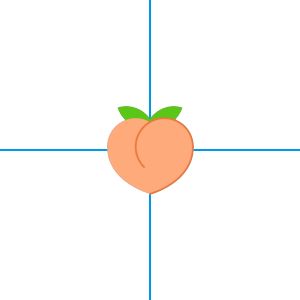
\includegraphics{1_introduction/1_3__intro_related_research_files/figure-pdf/unnamed-chunk-2-1.pdf}

}

\end{figure}

\part{Methods}

\hypertarget{sec-data}{%
\chapter{Data collection}\label{sec-data}}

\hypertarget{mpx-nyc-person-place-network-mapper}{%
\section{MPX NYC Person-Place Network
Mapper}\label{mpx-nyc-person-place-network-mapper}}

\begin{figure}

{\centering \includegraphics{2_methods/../_const/images/image_app_graphic.png}

}

\caption{\label{fig-mapinputformat}Map input question format developed
for MPX NYC}

\end{figure}

Data were collected using a custom designed survey instrument we call
the MPX NYC Person-Place Network Mapper. The Person-Place Network Map
question was designed to safely elicit sensitive spatial information
from survey participants. It displays a map with detailed geographic
information including place names, roads, and neighborhood names (see
Figure~\ref{fig-mapinputformat}).

To enter spatial information, the participant is prompted to identify
places of a certain type by tapping on the map. Each time the
participant taps the map, a marker appears where they tapped, and a
pop-up window asks questions about the most recently identified
location. To ensure anonymity, the survey tool coarsens spatial data to
the census tract level before sending them to the study database. Census
tracts are non-overlapping spatial units that partition the United
States into areas ranging from \(2500\) to \(8000\) in population size
(US Census 2022).

\hypertarget{mpx-nyc-marketing-and-communication}{%
\section{MPX NYC marketing and
communication}\label{mpx-nyc-marketing-and-communication}}

\begin{figure}

{\centering \includegraphics{2_methods/../_const/images/image_campaign_graphic.png}

}

\caption{\label{fig-options}Options for visual identity of MPX NYC''}

\end{figure}

We invested in a bilingual, culturally competent communication campaign
in collaboration with a marketing agency. As a starting point, the
RESPND-MI team suggested a campaign that playfully uses emojis that have
sexual connotations in queer and trans communities, and that integrates
LGBT social media influencers as a communication channel. Participants
were recruited via paid and donated advertising placed through Grindr,
Twitter, Instagram, and outdoor electronic billboards.

\hypertarget{consent-and-ethical-approval}{%
\section{Consent and ethical
approval}\label{consent-and-ethical-approval}}

Prospective participants read and responded to a consent statement
before being able to take the survey. The study, including marketing
materials and software, was reviewed and approved by the T.H. Chan
School of Public Health Institutional Review Board (IRB22-0761).

\hypertarget{participants-and-setting}{%
\section{Participants and setting}\label{participants-and-setting}}

Potential participants were included in the study if they consented to
participate, were over 18 years of age, identified as transgender, gay,
bisexual, or as men who have sex with other men, and were in New York
City in the four weeks preceding their participation. Potential
participants were excluded if they were younger than 18 years of age or
they withdrew consent.

\hypertarget{translation}{%
\section{Translation}\label{translation}}

All study materials were professionally translated from English to
Spanish. The translation was reviewed by six professionals in
health-related fields whose primary language is Spanish.

\begin{Shaded}
\begin{Highlighting}[]
\FunctionTok{plot\_icon}\NormalTok{(}\AttributeTok{icon\_name =} \StringTok{"devil"}\NormalTok{, }\AttributeTok{color =} \StringTok{"dark\_orange"}\NormalTok{, }\AttributeTok{shape =} \DecValTok{16}\NormalTok{, }\AttributeTok{alpha =} \FloatTok{0.1}\NormalTok{)}
\end{Highlighting}
\end{Shaded}

\begin{figure}[H]

{\centering 
\includegraphics{2_methods/2_2_methods_data_files/figure-pdf/unnamed-chunk-2-1.pdf}

}

\end{figure}

\hypertarget{sec-measures}{%
\chapter{Measures}\label{sec-measures}}

\begin{Shaded}
\begin{Highlighting}[]
\FunctionTok{make\_example\_network\_data}\NormalTok{(}\StringTok{"bipartite"}\NormalTok{) }\SpecialCharTok{|\textgreater{}}
  \FunctionTok{plot\_example\_network}\NormalTok{(targets}\SpecialCharTok{::}\FunctionTok{tar\_read}\NormalTok{(config\_list)) }\SpecialCharTok{+}
\NormalTok{  ggplot2}\SpecialCharTok{::}\FunctionTok{coord\_cartesian}\NormalTok{(}\AttributeTok{xlim=}\FunctionTok{c}\NormalTok{(}\SpecialCharTok{{-}}\DecValTok{2}\NormalTok{,}\DecValTok{3}\NormalTok{), }\AttributeTok{ylim=}\FunctionTok{c}\NormalTok{(}\SpecialCharTok{{-}}\FloatTok{1.2}\NormalTok{,}\FloatTok{1.2}\NormalTok{)) }\SpecialCharTok{+}
  \FunctionTok{theme\_mpxnyc\_blank}\NormalTok{() }\SpecialCharTok{+}
\NormalTok{  ggplot2}\SpecialCharTok{::}\FunctionTok{theme}\NormalTok{(}
    \AttributeTok{plot.margin =}\NormalTok{ ggplot2}\SpecialCharTok{::}\FunctionTok{margin}\NormalTok{(}\DecValTok{0}\NormalTok{,}\DecValTok{0}\NormalTok{,}\DecValTok{0}\NormalTok{,}\DecValTok{0}\NormalTok{)}
\NormalTok{  )}
\end{Highlighting}
\end{Shaded}

\begin{figure}[H]

{\centering 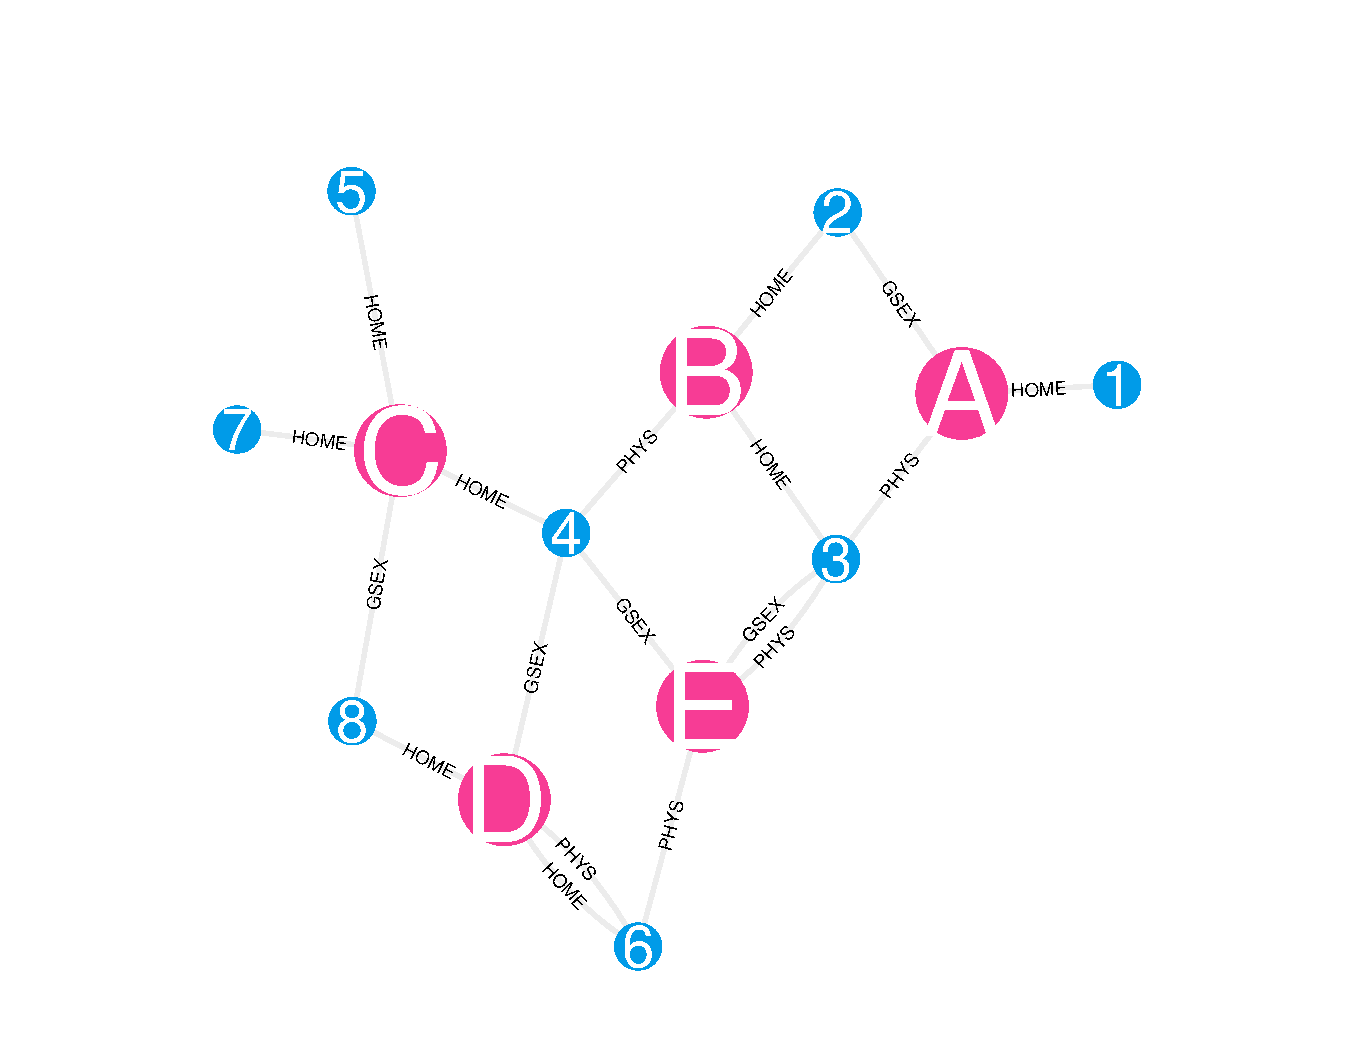
\includegraphics{2_methods/2_3_methods_measures_files/figure-pdf/fig-example-bipartite-1.pdf}

}

\caption{\label{fig-example-bipartite}Sample person-place network}

\end{figure}

\hypertarget{data-mpx-nyc-participant-community-network}{%
\section{Data: MPX NYC participant-community
network}\label{data-mpx-nyc-participant-community-network}}

The MPX NYC participant community network is a network with community
districts and individuals as nodes, and ties between pairs consisting of
one individual and one community district. While spatial data were
collected using census tract identifiers, the unit of spatial analysis
is the community district. Community districts are spatial units that
divide New York City into regions which are nested by the five boroughs
of New York City, and which in turn nest census tracts.

A tie indicates that the individual as some relation with the community
district. This relation can be residence or group contact. Related to
this network are the community district network and participant network,
described below.

\hypertarget{mpx-nyc-community-district-network}{%
\subsection{MPX NYC community district
network}\label{mpx-nyc-community-district-network}}

\begin{Shaded}
\begin{Highlighting}[]
  \FunctionTok{plot\_example\_network}\NormalTok{(}\FunctionTok{make\_example\_network\_data}\NormalTok{(}\StringTok{"places"}\NormalTok{), targets}\SpecialCharTok{::}\FunctionTok{tar\_read}\NormalTok{(config\_list))  }\SpecialCharTok{+}
  \FunctionTok{theme\_mpxnyc\_blank}\NormalTok{() }
\end{Highlighting}
\end{Shaded}

\begin{figure}[H]

{\centering 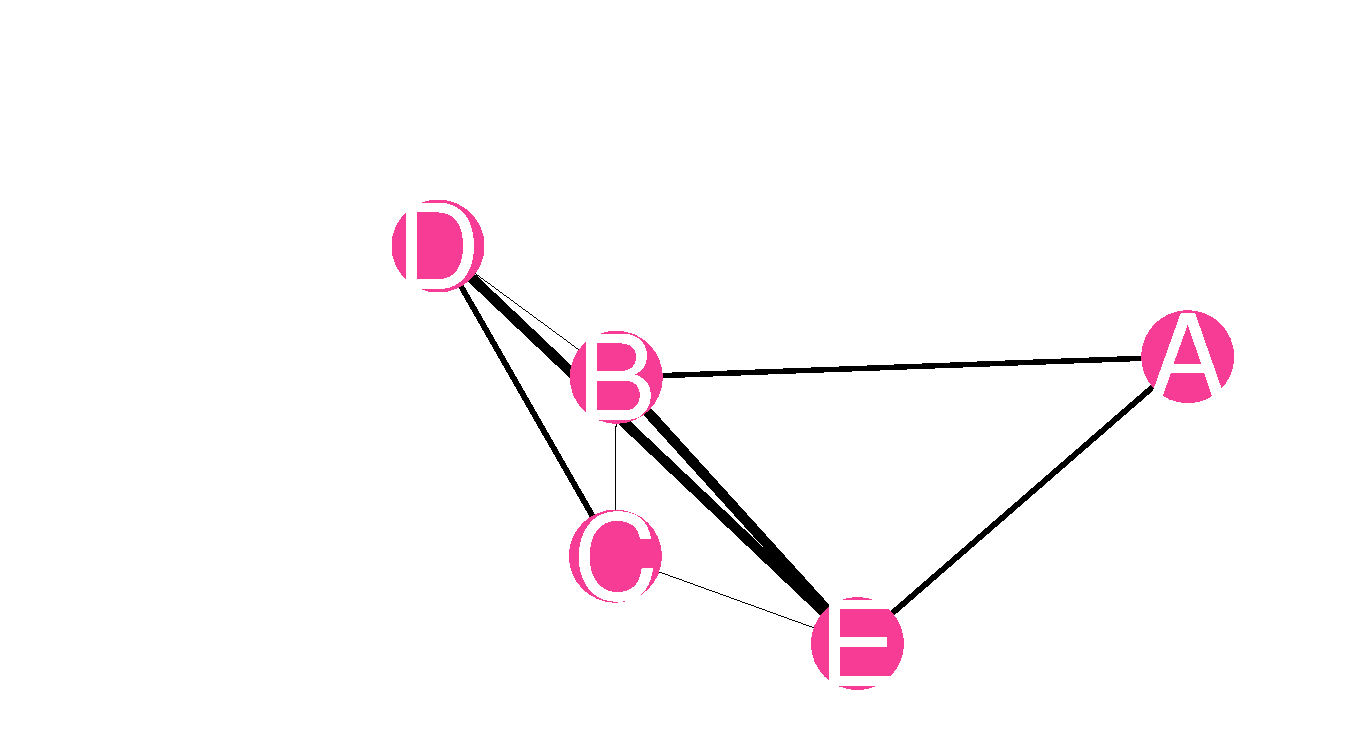
\includegraphics{2_methods/2_3_methods_measures_files/figure-pdf/fig-example-community-1.pdf}

}

\caption{\label{fig-example-community}Sample place-place network}

\end{figure}

The MPX NYC community district network is a network with community
districts as nodes. A weighted tie between two nodes indicates that the
two community districts both have at least one MPX NYX participant who
has a residence or community district in both places. The weight is
given by the count of such individuals. Of interest is the influence
each community district has in city-wide outbreak dynamics. It is
measured using community district social and spatial reach.

\hypertarget{mpx-nyc-participant-network}{%
\subsection{MPX NYC participant
network}\label{mpx-nyc-participant-network}}

\begin{Shaded}
\begin{Highlighting}[]
\FunctionTok{make\_example\_network\_data}\NormalTok{(}\StringTok{"people"}\NormalTok{) }\SpecialCharTok{|\textgreater{}}
  \FunctionTok{plot\_example\_network}\NormalTok{(targets}\SpecialCharTok{::}\FunctionTok{tar\_read}\NormalTok{(config\_list)) }\SpecialCharTok{+}
  \FunctionTok{theme\_mpxnyc\_blank}\NormalTok{()}
\end{Highlighting}
\end{Shaded}

\begin{figure}[H]

{\centering \includegraphics{2_methods/2_3_methods_measures_files/figure-pdf/fig-example-participant-1.pdf}

}

\caption{\label{fig-example-participant}Sample person-person network}

\end{figure}

We examined the patterning of shared physical context among participants
using the MPX NYC participant network. In this network, survey
participants are represented as nodes. A weighted edge indicates that
the individuals represented by the nodes have at least one residence or
contact venue in a common community district. The edge weight is given
by the count of community districts the pair share. Of interest are the
overall connectedness of the network and the pattern of connection
across different subgroups.

\hypertarget{node-characteristics}{%
\section{Node characteristics}\label{node-characteristics}}

\hypertarget{individual-measures}{%
\subsection{Individual measures}\label{individual-measures}}

We measured participant demographics age, race, sex assigned at birth,
gender identity, sexual orientation, and community district of
residence; health-related questions on HIV status, viral suppression,
STI-related symptoms, PrEP use, and mpox vaccination status; and
questions related to social and sexual connection with queer and
transgender communities: count of recent individual sex contacts, count
of recent individual physical (non-sexual) contacts, count of recent
important social contacts, and any recent physical or sexual contact in
a group setting.

\hypertarget{gender-modality}{%
\subsubsection{Gender modality}\label{gender-modality}}

Gender modality was measured using a two-step approach: first, we
solicited the participant's current gender (man, woman, trans man, trans
woman, non-binary, other), and then sex assigned at birth (male, female,
other). We then constructed a gender modality variable as follows:

\begin{Shaded}
\begin{Highlighting}[]
\FunctionTok{data.frame}\NormalTok{(}
  \AttributeTok{Level =} \FunctionTok{c}\NormalTok{(}
              \StringTok{"Cisgender man"}\NormalTok{, }
              \StringTok{"Cisgender woman"}\NormalTok{,}
              \StringTok{"Transgender man"}\NormalTok{,}
              \StringTok{"Transgender woman"}\NormalTok{,}
              \StringTok{"Transgender man"}\NormalTok{,}
              \StringTok{"Transgender woman"}\NormalTok{,}
              \StringTok{"Non{-}binary"}\NormalTok{,}
              \StringTok{"Another demographic"}
\NormalTok{              ),}
  \AttributeTok{Condition =} \FunctionTok{c}\NormalTok{(}
                \StringTok{"gender is \textquotesingle{}man\textquotesingle{} and assigned sex is \textquotesingle{}male\textquotesingle{} "}\NormalTok{, }
                \StringTok{"gender is \textquotesingle{}woman\textquotesingle{} and assigned sex is \textquotesingle{}female\textquotesingle{}"}\NormalTok{,}
                \StringTok{"gender is \textquotesingle{}man\textquotesingle{} and assigned sex is \textquotesingle{}female\textquotesingle{}"}\NormalTok{,}
                \StringTok{"gender is \textquotesingle{}woman\textquotesingle{} and assigned sex is \textquotesingle{}male\textquotesingle{}"}\NormalTok{,}
                \StringTok{"gender is \textquotesingle{}trans man\textquotesingle{} and sex is any value"}\NormalTok{,}
                \StringTok{"gender is \textquotesingle{}trans woman\textquotesingle{} and sex is any value"}\NormalTok{,}
                \StringTok{"gender is \textquotesingle{}non{-}binary\textquotesingle{} and sex is any value"}\NormalTok{,}
                \StringTok{"gender is \textquotesingle{}other\textquotesingle{} and sex is any value"}
\NormalTok{                )}
             
\NormalTok{) }\SpecialCharTok{|\textgreater{}}
\NormalTok{  gt}\SpecialCharTok{::}\FunctionTok{gt}\NormalTok{()}
\end{Highlighting}
\end{Shaded}

\hypertarget{tbl-gendermodality}{}
\begin{longtable}{ll}
\caption{\label{tbl-gendermodality}\_construction of gender modality variable }\tabularnewline

\toprule
Level & Condition \\ 
\midrule\addlinespace[2.5pt]
Cisgender man & gender is 'man' and assigned sex is 'male'  \\ 
Cisgender woman & gender is 'woman' and assigned sex is 'female' \\ 
Transgender man & gender is 'man' and assigned sex is 'female' \\ 
Transgender woman & gender is 'woman' and assigned sex is 'male' \\ 
Transgender man & gender is 'trans man' and sex is any value \\ 
Transgender woman & gender is 'trans woman' and sex is any value \\ 
Non-binary & gender is 'non-binary' and sex is any value \\ 
Another demographic & gender is 'other' and sex is any value \\ 
\bottomrule
\end{longtable}

\hypertarget{race-gender}{%
\subsubsection{Race-gender}\label{race-gender}}

We created a Race-gender variable which is a categorical variable with
levels identical to the gender modality with one modification: instead
of having all cisgender men in one level we divided the group up into
white cisgender men, Latinx cisgender men, Black cisgender men, and
under the category Other cisgender men, we grouped Asian, Pacific
Islander and other cisgender men.

\hypertarget{community-district-measures}{%
\subsection{Community district
measures}\label{community-district-measures}}

\hypertarget{social-reach}{%
\subsubsection{Social reach}\label{social-reach}}

For a given community district, social reach is defined as the sum of
edge weights for edges connecting that community district to individuals
(in the MPX NYC spatial participant network). It quantifies the volume
or level of contact in the community district.

\hypertarget{spatial-reach}{%
\subsubsection{Spatial reach}\label{spatial-reach}}

For a given community district spatial reach is defined as the sum of
edge weights for edges connecting that community district to others (in
the MPX NYC community district network. It quantifies the volume or
level of exchange of individuals between a particular community district
and others.

\hypertarget{edge-characteristics}{%
\section{Edge characteristics}\label{edge-characteristics}}

\hypertarget{residence-edges}{%
\subsection{Residence edges}\label{residence-edges}}

All participants were asked the location of their residence through the
Person-Place Network Map question. Each participant's residences is
represented as an edge between the participant and the community
district containing their residence.

\hypertarget{contact-venue-edges}{%
\subsection{Contact venue edges}\label{contact-venue-edges}}

Participants who indicated recent physical or sexual contact in a group
setting were asked for the locations of each of the places where the
contact happened. We call these contact places. They are each
represented as an edge between the participant and the community
district containing the contact place.

\hypertarget{venue-type}{%
\subsubsection{Venue type}\label{venue-type}}

Participants were asked the type of venue each contact place was (dance
party, sex party, darkroom, sport game, concert, theatre/show, private
residence, sex club, bathhouse, park, something else).

\hypertarget{sexual-contact}{%
\subsubsection{Sexual contact}\label{sexual-contact}}

Participants were also asked if they had sexual contact at each contact
place.

\hypertarget{distance-from-home}{%
\subsubsection{Distance from home}\label{distance-from-home}}

We constructed an approximate measure of the distance between residence
and contact venue by categorizing venues into those that are in the same
community district as the residence; in a different community district
but the same borough; or in a different borough. We refer to this
measure as distance from home.

\hypertarget{network-characteristics}{%
\section{Network characteristics}\label{network-characteristics}}

\hypertarget{size-of-largest-connected-component}{%
\subsubsection{Size of largest connected
component}\label{size-of-largest-connected-component}}

We measure connectedness using the proportion of nodes in the largest
connected component (LCC) of the MPX NYC participant network. In a
network, a connected component is a subset of nodes such that each node
in the subset is reachable from any other node in the subset, and such
that there are no nodes outside the subset which are reachable from a
node inside it. By ``reachable'', we mean possible to reach by tracing a
path from one node to another over existing network ties. We consider a
network with a larger LCC to be better connected than a network with a
smaller LCC.

\hypertarget{spatial-mixing-ratio}{%
\subsubsection{Spatial mixing ratio}\label{spatial-mixing-ratio}}

We measure patterns of mixing between a pair of distict subgroups of
participants using the spatial mixing ratio. It is a positive real
number which is greater than 1 if individuals in the first subgroup tend
to live and play in community districts that individuals in the second
subgroup do. It is defined as the average (calculated across
individuals) spatial preference of the first group for the second group,
divided by the prevalence of the second group. For a given individual,
spatial preference for a given group is defined as the sum of the
weights of the edges connecting to nodes of the second group, divided by
the total sum weights.

\begin{Shaded}
\begin{Highlighting}[]
\FunctionTok{plot\_icon}\NormalTok{(}\AttributeTok{icon\_name =} \StringTok{"devil"}\NormalTok{, }\AttributeTok{color =} \StringTok{"dark\_orange"}\NormalTok{, }\AttributeTok{shape =} \DecValTok{16}\NormalTok{, }\AttributeTok{alpha =} \FloatTok{0.1}\NormalTok{)}
\end{Highlighting}
\end{Shaded}

\begin{figure}[H]

{\centering 
\includegraphics{2_methods/2_3_methods_measures_files/figure-pdf/unnamed-chunk-6-1.pdf}

}

\end{figure}

\hypertarget{sec-analysis}{%
\chapter{Statistical Analysis}\label{sec-analysis}}

\hypertarget{descriptive-statistics}{%
\section{Descriptive statistics}\label{descriptive-statistics}}

We tabulated participant characteristics against group contact, and
visualized the distribution of sexual orientation categories across
levels of the race-gender variable. We also tabulated contact venue
characteristics against sexual contact, and further visualized venue
type against distance from home in addition to sexual contact.

To understand how participants move across community districts from home
to contact places, we cross-tabulated home community district (the
community district of the participants' residence) against contact place
community district and visualized the resulting table. To identify
community districts that tend to receive more participants from
residences in outside community districts, and those which tend to send
participants, we subtracted the proportion of residences in each
community district from the proportion of contact venues. The result of
this calculation is shown as a bar graph.

Finally, we calculated the spatial mixing coefficient across groups
defined by age, sexual orientation, and race-gender to understand how
individuals in subgroups defined by these variables interact in space.

To illustrate how the pattern of interaction among queer and trans
people should inform early responses to novel infectious diseases, we
examined the impact of a simplified, spatially-targeted intervention to
immunize the population represented by the MPX NYC participants against
a novel pathogen. We examine the impact of two different intervention
strategies on two population outcome measures of interest

\hypertarget{outbreak-control-strategies}{%
\section{Outbreak control
strategies}\label{outbreak-control-strategies}}

In this hypothetical intervention, community districts are ordered by
priority and are immunized one at a time, beginning with the highest
priority community district. We assume that to immunize a community
district is to immunize each individual who has a contact venue or
residence in that community district. We assume that once a person is
immunized, they are unable to acquire or transmit the pathogen, and we
assume that everyone can only be immunized once. We assessed two
strategies for prioritizing community districts: the
contact-neutralizing strategy and the movement-neutralizing strategy.

\hypertarget{contact-neutralizing-strategy}{%
\subsection{Contact neutralizing
strategy}\label{contact-neutralizing-strategy}}

In the contact-neutralizing strategy, we rank districts according to the
number of contact venues and residences they contain (counting only the
residences of participants who reported group contact, and who are not
yet immunized). This strategy prioritizes community districts with a
high amount of sexual or physical contact for immunization. It attempts
to immunize as many people in as few community districts as possible.

\hypertarget{movement-neutralizing-strategy}{%
\subsection{Movement neutralizing
strategy}\label{movement-neutralizing-strategy}}

In the movement-neutralizing strategy, we rank community districts by
their spatial centrality. This strategy prioritizes community districts
with a high level of connection to other community districts for
immunization. It attempts to immunize the community districts that are
potential hubs for the dissemination of the pathogen across the city
early to geographically contain the outbreak.

\hypertarget{outbreak-control-outcomes}{%
\section{Outbreak control outcomes}\label{outbreak-control-outcomes}}

For each community district immunized, we updated the MPX NYC
participant network by removing nodes that represent immunized
individuals. We then calculated the two outcomes each time: spatial
efficiency, and spatial network impact.

\hypertarget{spatial-efficiency}{%
\subsection{Spatial efficiency}\label{spatial-efficiency}}

Spatial efficiency is defined as the total count of immunized
individuals divided by the count of immunized community districts. To
illustrate differences in spatial efficiency across intervention
strategies, we visualized the number of community districts it would
take to immunize 33\% of the population, and 66\% of the population
respectively.

\hypertarget{spatial-network-impact}{%
\subsection{Spatial network impact}\label{spatial-network-impact}}

Spatial network impact is defined as the proportion of individuals
included in the largest connected component of the MPX NYC participant
network. To illustrate differences in spatial network impact across
intervention strategies, for each additional community district
immunized, we plotted the proportions of individuals who are immunized,
unimmunized and in the largest connected component, and unimmunized but
outside of the largest connected component, respectively.

\hypertarget{statistical-inference}{%
\section{Statistical inference}\label{statistical-inference}}

\begin{Shaded}
\begin{Highlighting}[]
\NormalTok{number\_reps }\OtherTok{\textless{}{-}}\NormalTok{ targets}\SpecialCharTok{::}\FunctionTok{tar\_read}\NormalTok{(config\_list)[[}\DecValTok{1}\NormalTok{]][[}\StringTok{"settings"}\NormalTok{]][[}\StringTok{"n\_reps\_graph"}\NormalTok{]]}
\end{Highlighting}
\end{Shaded}

We used the bootstrap to estimate confidence intervals, resampling
participants 20 times with replacement.

\begin{Shaded}
\begin{Highlighting}[]
\FunctionTok{plot\_icon}\NormalTok{(}\AttributeTok{icon\_name =} \StringTok{"droplets"}\NormalTok{, }\AttributeTok{color =} \StringTok{"dark\_pink"}\NormalTok{, }\AttributeTok{shape =} \DecValTok{16}\NormalTok{, }\AttributeTok{alpha =} \FloatTok{0.1}\NormalTok{)}
\end{Highlighting}
\end{Shaded}

\begin{figure}[H]

{\centering 
\includegraphics{2_methods/2_4_methods_statistical_analysis_files/figure-pdf/unnamed-chunk-3-1.pdf}

}

\end{figure}

\part{Results}

\hypertarget{sec-participants}{%
\chapter{People}\label{sec-participants}}

\begin{Shaded}
\begin{Highlighting}[]
\FunctionTok{make\_plotdata\_racegender\_radar\_grid}\NormalTok{() }\SpecialCharTok{|\textgreater{}}
  \FunctionTok{plot\_radar\_grid}\NormalTok{() }\SpecialCharTok{+}
\NormalTok{  ggplot2}\SpecialCharTok{::}\FunctionTok{scale\_y\_continuous}\NormalTok{(}\AttributeTok{breaks =} \FunctionTok{c}\NormalTok{(}\DecValTok{0}\NormalTok{,}\FloatTok{0.25}\NormalTok{, }\FloatTok{0.50}\NormalTok{, }\DecValTok{1}\NormalTok{), }\AttributeTok{limits =} \FunctionTok{c}\NormalTok{(}\SpecialCharTok{{-}}\FloatTok{0.5}\NormalTok{, }\DecValTok{1}\NormalTok{)) }\SpecialCharTok{+}
  \FunctionTok{scale\_fill\_mpxnyc}\NormalTok{(}\AttributeTok{name =} \StringTok{""}\NormalTok{) }\SpecialCharTok{+}
  \FunctionTok{theme\_mpxnyc\_radar\_people}\NormalTok{() }
\end{Highlighting}
\end{Shaded}

\begin{figure}[H]

{\centering 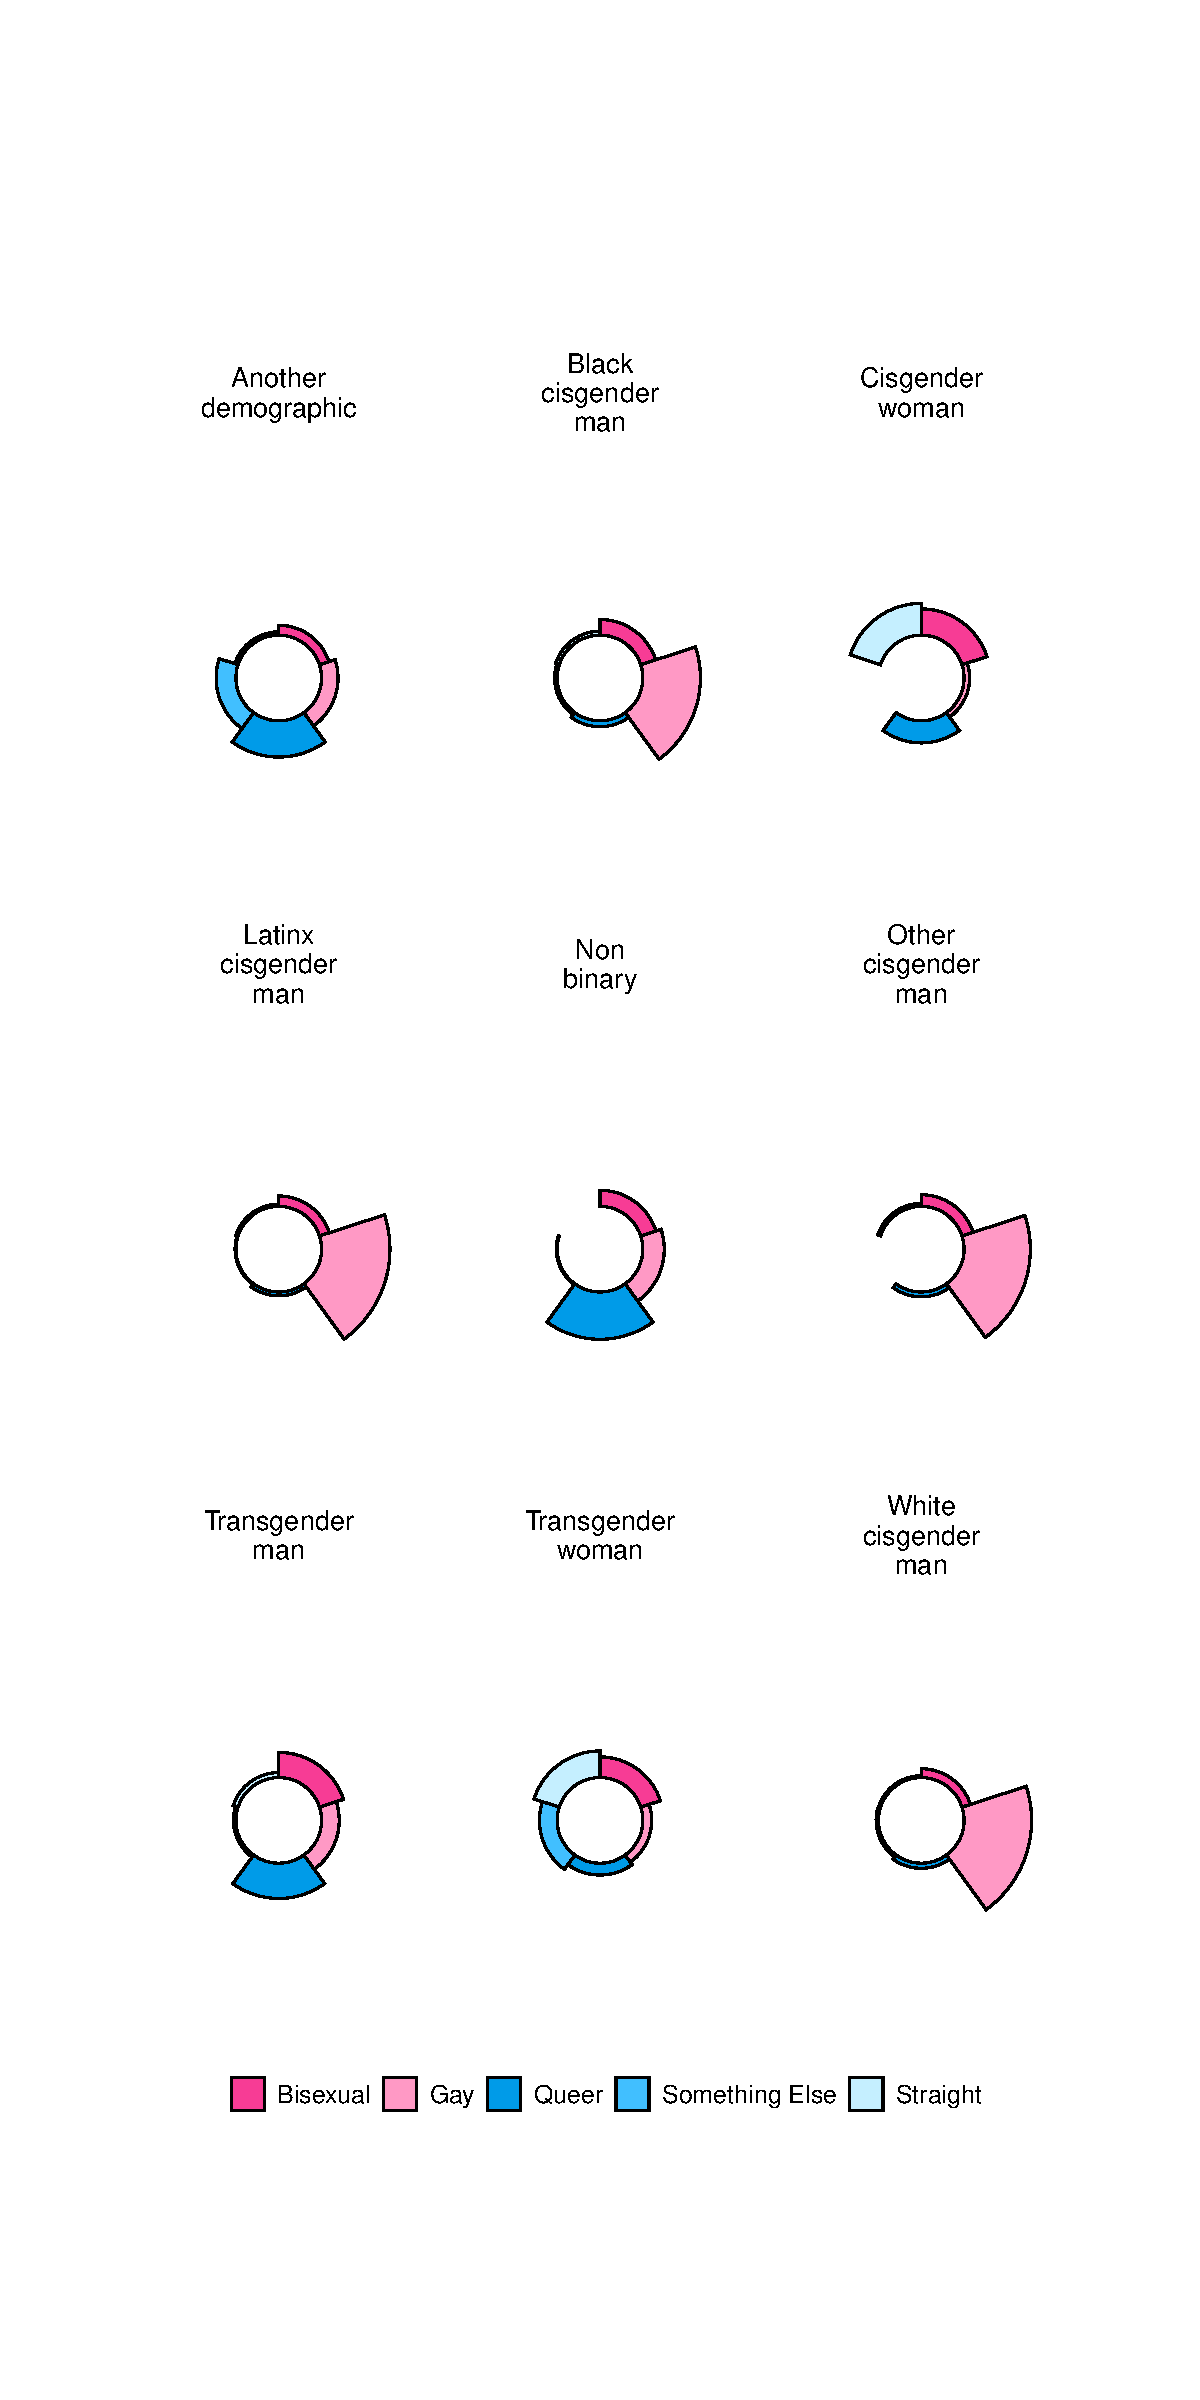
\includegraphics{3_results/3_1__results_participants_files/figure-pdf/fig-racegender-radar-grid-1.pdf}

}

\caption{\label{fig-racegender-radar-grid}Sexual orientation of MPX NYC
participants by race and gender}

\end{figure}

Participants who reported recent physical or sexual contact in a group
setting (group contact) were slightly younger than those who did not.
They were more likely to identify as gay and less likely to identify as
straight. Surprisingly, they were less likely to have been recruited
through a Grindr advertisement and more likely to have been recruited
before the first Grindr pop-up advertisement on 30 August 2022.

These participants did not differ from the rest in terms of HIV status
or HIV viral suppression, but they were more likely to have at least one
STI symptom, and showed higher utilization of PrEP, mpox testing, and
mpox vaccine. They were more closely connected with the queer and trans
community, reporting more contact with friends, more physical contact
partners and more sexual contact partners. They spent more time
travelling to hookups than participants who had not had recent contact
in a group setting.

\hypertarget{demographics}{%
\section{Demographics}\label{demographics}}

MPX NYC participants are demographically diverse (see
Table~\ref{tbl-demographics} and
Figure~\ref{fig-racegender-radar-grid}). Over 50\% of participants were
between the ages of 18-34 at the time of the survey. Two fifths were
white cisgender men, about 15\% were latinx cisgender men, and 10\% were
black cisgender men. About 5\% of participants were transgender (with
slightly over half being transgender men). Non-binary individuals
comprised 7\% of participants. Two-thirds of participants identified as
gay, 14\% as bisexual, and 12\% as queer. Just under half of
participants resided in the borough of Manhattan, and one third in
Brooklyn.

This diversity of subgroups implies different strategies for
communication, and possibly different health interventions. For
instance, the sexual orientation of participants differed markedly by
gender (see Figure~\ref{fig-racegender-radar-grid}). The vast majority
of cisgender men identified as gay, with some identifying as bisexual.
Transgender men, on the other hand, were most likely to identify as
queer, followed by bisexual or gay. Transgender women tended to identify
as straight, bisexual, or other sexual orientations. Cisgender women
participants tended to be straight, followed by bisexual, followed by
queer. For non-binary people, most identified as queer, followed by gay
and bisexual.

\begin{Shaded}
\begin{Highlighting}[]
\FunctionTok{make\_tabledata\_demographics}\NormalTok{() }\SpecialCharTok{|\textgreater{}}
  \FunctionTok{draw\_table\_by\_groupSex}\NormalTok{()}
\end{Highlighting}
\end{Shaded}

\hypertarget{tbl-demographics}{}
\setlength{\LTpost}{0mm}
\begin{longtable}{lcccc}
\caption{\label{tbl-demographics}Participants in MPX NYC Study by Sex / Physical Contact in Congregate
Setting in past 4 weeks }\tabularnewline

\toprule
 & \multicolumn{3}{c}{\textbf{Physical or sexual contact in group setting in past 4 weeks}} &  \\ 
\cmidrule(lr){2-4}
\textbf{Variable} & \textbf{Yes}\\
N = 530\textsuperscript{\textit{1}} & \textbf{No}\\
N = 774\textsuperscript{\textit{1}} & \textbf{Overall}\\
N = 1,304\textsuperscript{\textit{1}} & \textbf{p-value}\textsuperscript{\textit{2}} \\ 
\midrule\addlinespace[2.5pt]
\textbf{Age} &  &  &  & <.001 \\ 
    18-24 & 92 (17\%) & 103 (13\%) & 195 (15\%) &  \\ 
    25-34 & 234 (44\%) & 304 (39\%) & 538 (41\%) &  \\ 
    35-44 & 135 (25\%) & 190 (25\%) & 325 (25\%) &  \\ 
    45-54 & 48 (9.1\%) & 97 (13\%) & 145 (11\%) &  \\ 
    55+ & 21 (4.0\%) & 80 (10\%) & 101 (7.7\%) &  \\ 
\textbf{Race} &  &  &  & 0.4 \\ 
    Another Group & 19 (3.6\%) & 40 (5.2\%) & 59 (4.5\%) &  \\ 
    Asian & 32 (6.0\%) & 52 (6.7\%) & 84 (6.4\%) &  \\ 
    Black & 60 (11\%) & 96 (12\%) & 156 (12\%) &  \\ 
    Latinx & 103 (19\%) & 128 (17\%) & 231 (18\%) &  \\ 
    Multi Racial & 37 (7.0\%) & 42 (5.4\%) & 79 (6.1\%) &  \\ 
    White & 279 (53\%) & 416 (54\%) & 695 (53\%) &  \\ 
\textbf{Gender identity} &  &  &  & 0.3 \\ 
    Cisgender Man & 427 (81\%) & 630 (81\%) & 1,057 (81\%) &  \\ 
    Non Binary & 39 (7.4\%) & 57 (7.4\%) & 96 (7.4\%) &  \\ 
    Transgender Man & 17 (3.2\%) & 17 (2.2\%) & 34 (2.6\%) &  \\ 
    Transgender Woman & 14 (2.6\%) & 15 (1.9\%) & 29 (2.2\%) &  \\ 
    Cisgender Woman & 19 (3.6\%) & 43 (5.6\%) & 62 (4.8\%) &  \\ 
    Another Demographic & 14 (2.6\%) & 12 (1.6\%) & 26 (2.0\%) &  \\ 
\textbf{Sexual orientation} &  &  &  & 0.010 \\ 
    Gay & 362 (68\%) & 498 (64\%) & 860 (66\%) &  \\ 
    Bisexual & 67 (13\%) & 119 (15\%) & 186 (14\%) &  \\ 
    Straight & 14 (2.6\%) & 50 (6.5\%) & 64 (4.9\%) &  \\ 
    Queer & 71 (13\%) & 88 (11\%) & 159 (12\%) &  \\ 
    Something Else & 16 (3.0\%) & 19 (2.5\%) & 35 (2.7\%) &  \\ 
\bottomrule
\end{longtable}
\begin{minipage}{\linewidth}
\textsuperscript{\textit{1}}n (\%)\\
\textsuperscript{\textit{2}}Pearson's Chi-squared test\\
\emph{Data source: MPX NYC 2022}\\
\end{minipage}

\hypertarget{connection}{%
\section{Connection}\label{connection}}

MPX NYC participants were deeply connected to queer and trans
communities in New York City (see Table~\ref{tbl-connection}). About
two-thirds reported being in recent (preceding 4 weeks) contact with 1 -
10 queer or trans friends. Only 20\% reported not being in contact.
About half of the participants had between 1 and 3 recent serial sex
partnerships with one fifth reporting four or more partners. About one
third of participants reported spending 16-30 minutes when traveling to
a hookup while a third spent more than 30 minutes. Almost one in four
participants reported having recent physical (non-sexual) contact with 2
or more individuals at the same time, and one third reported having had
no contact.

Among all MPX NYC participants, 40\% (530) reported reported having had
sex or physical contact with two or more people at the same time. These
participants identified \(604\) venues at which they had contact. These
contact venues are examined in the next section.

\begin{Shaded}
\begin{Highlighting}[]
\FunctionTok{make\_tabledata\_connection}\NormalTok{() }\SpecialCharTok{|\textgreater{}}
  \FunctionTok{draw\_table\_by\_groupSex}\NormalTok{()}
\end{Highlighting}
\end{Shaded}

\hypertarget{tbl-connection}{}
\setlength{\LTpost}{0mm}
\begin{longtable}{lcccc}
\caption{\label{tbl-connection}Participants in MPX NYC Study by Sex / Physical Contact in Congregate
Setting in past 4 weeks }\tabularnewline

\toprule
 & \multicolumn{3}{c}{\textbf{Physical or sexual contact in group setting in past 4 weeks}} &  \\ 
\cmidrule(lr){2-4}
\textbf{Variable} & \textbf{Yes}\\
N = 530\textsuperscript{\textit{1}} & \textbf{No}\\
N = 774\textsuperscript{\textit{1}} & \textbf{Overall}\\
N = 1,304\textsuperscript{\textit{1}} & \textbf{p-value}\textsuperscript{\textit{2}} \\ 
\midrule\addlinespace[2.5pt]
\textbf{Recent important social contacts} &  &  &  & <.001 \\ 
    0 & 64 (12\%) & 155 (20\%) & 219 (17\%) &  \\ 
    1-5 & 206 (39\%) & 333 (43\%) & 539 (41\%) &  \\ 
    6-10 & 136 (26\%) & 167 (22\%) & 303 (23\%) &  \\ 
    11-15 & 49 (9.2\%) & 41 (5.3\%) & 90 (6.9\%) &  \\ 
    16+ & 75 (14\%) & 78 (10\%) & 153 (12\%) &  \\ 
\textbf{Recent physical contacts} &  &  &  & <.001 \\ 
    0 & 98 (18\%) & 301 (39\%) & 399 (31\%) &  \\ 
    1 & 68 (13\%) & 191 (25\%) & 259 (20\%) &  \\ 
    2 & 66 (12\%) & 105 (14\%) & 171 (13\%) &  \\ 
    3 & 46 (8.7\%) & 64 (8.3\%) & 110 (8.4\%) &  \\ 
    4 & 47 (8.9\%) & 32 (4.1\%) & 79 (6.1\%) &  \\ 
    5+ & 205 (39\%) & 81 (10\%) & 286 (22\%) &  \\ 
\textbf{Recent individual sex contacts} &  &  &  & <.001 \\ 
    0 & 48 (9.1\%) & 272 (35\%) & 320 (25\%) &  \\ 
    1 & 86 (16\%) & 258 (33\%) & 344 (26\%) &  \\ 
    2 & 96 (18\%) & 110 (14\%) & 206 (16\%) &  \\ 
    3 & 82 (15\%) & 62 (8.0\%) & 144 (11\%) &  \\ 
    4 & 62 (12\%) & 29 (3.7\%) & 91 (7.0\%) &  \\ 
    5+ & 156 (29\%) & 43 (5.6\%) & 199 (15\%) &  \\ 
\textbf{Hookup travel time} &  &  &  & <.001 \\ 
    0-15 min & 121 (23\%) & 262 (34\%) & 383 (29\%) &  \\ 
    16-30 min & 221 (42\%) & 270 (35\%) & 491 (38\%) &  \\ 
    31-45 min & 71 (13\%) & 88 (11\%) & 159 (12\%) &  \\ 
    45+ min & 117 (22\%) & 154 (20\%) & 271 (21\%) &  \\ 
\bottomrule
\end{longtable}
\begin{minipage}{\linewidth}
\textsuperscript{\textit{1}}n (\%)\\
\textsuperscript{\textit{2}}Pearson's Chi-squared test\\
\emph{Data source: MPX NYC 2022}\\
\end{minipage}

\hypertarget{health}{%
\section{Health}\label{health}}

In terms of health status and health services, one in ten participants
reported living with HIV - the overwhelming majority were virally
suppressed (see Table~\ref{tbl-health}). In addition, about 16\%
reported at least one STI symptom. Two out of five participants were on
PrEP at the time they took the survey. Two-thirds had received the MPOX
vaccine, though only 8\% had received MPOX testing.

\begin{Shaded}
\begin{Highlighting}[]
\FunctionTok{make\_tabledata\_health}\NormalTok{() }\SpecialCharTok{|\textgreater{}}
  \FunctionTok{draw\_table\_by\_groupSex}\NormalTok{()}
\end{Highlighting}
\end{Shaded}

\hypertarget{tbl-health}{}
\setlength{\LTpost}{0mm}
\begin{longtable}{lcccc}
\caption{\label{tbl-health}Participants in MPX NYC Study by Sex / Physical Contact in Congregate
Setting in past 4 weeks }\tabularnewline

\toprule
 & \multicolumn{3}{c}{\textbf{Physical or sexual contact in group setting in past 4 weeks}} &  \\ 
\cmidrule(lr){2-4}
\textbf{Variable} & \textbf{Yes}\\
N = 530\textsuperscript{\textit{1}} & \textbf{No}\\
N = 774\textsuperscript{\textit{1}} & \textbf{Overall}\\
N = 1,304\textsuperscript{\textit{1}} & \textbf{p-value}\textsuperscript{\textit{2}} \\ 
\midrule\addlinespace[2.5pt]
\textbf{HIV status} &  &  &  & 0.072 \\ 
    Living with HIV & 60 (11\%) & 81 (10\%) & 141 (11\%) &  \\ 
    Not living with HIV & 447 (84\%) & 676 (87\%) & 1,123 (86\%) &  \\ 
    Unsure & 23 (4.3\%) & 17 (2.2\%) & 40 (3.1\%) &  \\ 
\textbf{HIV supressed} &  &  &  & 0.15 \\ 
    Yes & 54 (90\%) & 78 (95\%) & 132 (93\%) &  \\ 
    No & 3 (5.0\%) & 4 (4.9\%) & 7 (4.9\%) &  \\ 
    Unsure & 3 (5.0\%) & 0 (0\%) & 3 (2.1\%) &  \\ 
    Unknown & 470 & 692 & 1,162 &  \\ 
\textbf{Any STI symptoms} & 118 (22\%) & 93 (12\%) & 211 (16\%) & <.001 \\ 
\textbf{PrEP user} & 252 (48\%) & 253 (33\%) & 505 (39\%) & <.001 \\ 
\textbf{MPOX tested} & 58 (11\%) & 47 (6.1\%) & 105 (8.1\%) & 0.001 \\ 
\textbf{MPOX vaccinated} & 409 (77\%) & 461 (60\%) & 870 (67\%) & <.001 \\ 
\bottomrule
\end{longtable}
\begin{minipage}{\linewidth}
\textsuperscript{\textit{1}}n (\%)\\
\textsuperscript{\textit{2}}Pearson's Chi-squared test; Fisher's exact test\\
\emph{Data source: MPX NYC 2022}\\
\end{minipage}

\hypertarget{study-recruitment}{%
\section{Study recruitment}\label{study-recruitment}}

The MPX NYC survey was open from 30 August to 15 November, 2022, but
recruited \(70\%\) participants in two 48 hour periods: half were
recruited from 30 to 31 Aug, and another 20\% from 10 to 11 September
(see Table~\ref{tbl-recruitment}). Over these periods, the MPX NYC
recruitment advertisements were shown to users of Grindr in New York
City upon logging on to the app.

\begin{Shaded}
\begin{Highlighting}[]
\FunctionTok{make\_table\_data\_recruitment}\NormalTok{()  }\SpecialCharTok{|\textgreater{}}
  \FunctionTok{draw\_table\_by\_groupSex}\NormalTok{()}
\end{Highlighting}
\end{Shaded}

\hypertarget{tbl-recruitment}{}
\setlength{\LTpost}{0mm}
\begin{longtable}{lcccc}
\caption{\label{tbl-recruitment}Participants in MPX NYC Study by Sex / Physical Contact in Congregate
Setting in past 4 weeks }\tabularnewline

\toprule
 & \multicolumn{3}{c}{\textbf{Physical or sexual contact in group setting in past 4 weeks}} &  \\ 
\cmidrule(lr){2-4}
\textbf{Variable} & \textbf{Yes}\\
N = 530\textsuperscript{\textit{1}} & \textbf{No}\\
N = 774\textsuperscript{\textit{1}} & \textbf{Overall}\\
N = 1,304\textsuperscript{\textit{1}} & \textbf{p-value}\textsuperscript{\textit{2}} \\ 
\midrule\addlinespace[2.5pt]
\textbf{Home borough} &  &  &  & 0.019 \\ 
    Bronx & 31 (5.8\%) & 66 (8.5\%) & 97 (7.4\%) &  \\ 
    Brooklyn & 176 (33\%) & 258 (33\%) & 434 (33\%) &  \\ 
    Manhattan & 259 (49\%) & 320 (41\%) & 579 (44\%) &  \\ 
    Queens & 58 (11\%) & 119 (15\%) & 177 (14\%) &  \\ 
    Staten Island & 6 (1.1\%) & 11 (1.4\%) & 17 (1.3\%) &  \\ 
\textbf{Recruitment channel} &  &  &  & 0.002 \\ 
    Grindr & 262 (49\%) & 444 (57\%) & 706 (54\%) &  \\ 
    Partner toolkit & 60 (11\%) & 82 (11\%) & 142 (11\%) &  \\ 
    Instagram & 47 (8.9\%) & 65 (8.4\%) & 112 (8.6\%) &  \\ 
    Twitter & 19 (3.6\%) & 43 (5.6\%) & 62 (4.8\%) &  \\ 
    Unknown & 142 (27\%) & 140 (18\%) & 282 (22\%) &  \\ 
\textbf{Survey date} &  &  &  & 0.041 \\ 
    30-31 Aug 2022 & 239 (45\%) & 372 (48\%) & 611 (47\%) &  \\ 
    01-10 Sep 2022 & 110 (21\%) & 118 (15\%) & 228 (17\%) &  \\ 
    10-11 Sep 2022 & 98 (18\%) & 171 (22\%) & 269 (21\%) &  \\ 
    12 Sep - 31 Nov 2022 & 83 (16\%) & 113 (15\%) & 196 (15\%) &  \\ 
\bottomrule
\end{longtable}
\begin{minipage}{\linewidth}
\textsuperscript{\textit{1}}n (\%)\\
\textsuperscript{\textit{2}}Pearson's Chi-squared test\\
\emph{Data source: MPX NYC 2022}\\
\end{minipage}

\begin{Shaded}
\begin{Highlighting}[]
\FunctionTok{plot\_icon}\NormalTok{(}\AttributeTok{icon\_name =} \StringTok{"peach"}\NormalTok{, }\AttributeTok{color =} \StringTok{"light\_green"}\NormalTok{, }\AttributeTok{shape =} \DecValTok{8}\NormalTok{)}
\end{Highlighting}
\end{Shaded}

\begin{figure}[H]

{\centering 
\includegraphics{3_results/3_1__results_participants_files/figure-pdf/unnamed-chunk-7-1.pdf}

}

\end{figure}

\hypertarget{sec-venues}{%
\chapter{Places}\label{sec-venues}}

\begin{Shaded}
\begin{Highlighting}[]
\FunctionTok{make\_plotdata\_placetype\_bar\_grid}\NormalTok{() }\SpecialCharTok{|\textgreater{}}
  \FunctionTok{plot\_radar\_stratified2}\NormalTok{() }\SpecialCharTok{+}
\NormalTok{  ggplot2}\SpecialCharTok{::}\FunctionTok{coord\_flip}\NormalTok{()  }\SpecialCharTok{+}
\NormalTok{  ggplot2}\SpecialCharTok{::}\FunctionTok{scale\_x\_discrete}\NormalTok{(}\AttributeTok{position =} \StringTok{"top"}\NormalTok{) }\SpecialCharTok{+}
\NormalTok{  ggplot2}\SpecialCharTok{::}\FunctionTok{scale\_y\_continuous}\NormalTok{(}\AttributeTok{labels =} \ControlFlowTok{function}\NormalTok{(x) scales}\SpecialCharTok{::}\FunctionTok{percent}\NormalTok{(}\FunctionTok{abs}\NormalTok{(x))) }\SpecialCharTok{+}
  \FunctionTok{scale\_fill\_mpxnyc}\NormalTok{(}\AttributeTok{name =} \StringTok{""}\NormalTok{) }\SpecialCharTok{+}
  \FunctionTok{theme\_mpxnyc\_radar\_places}\NormalTok{() }
\end{Highlighting}
\end{Shaded}

\begin{figure}[H]

{\centering 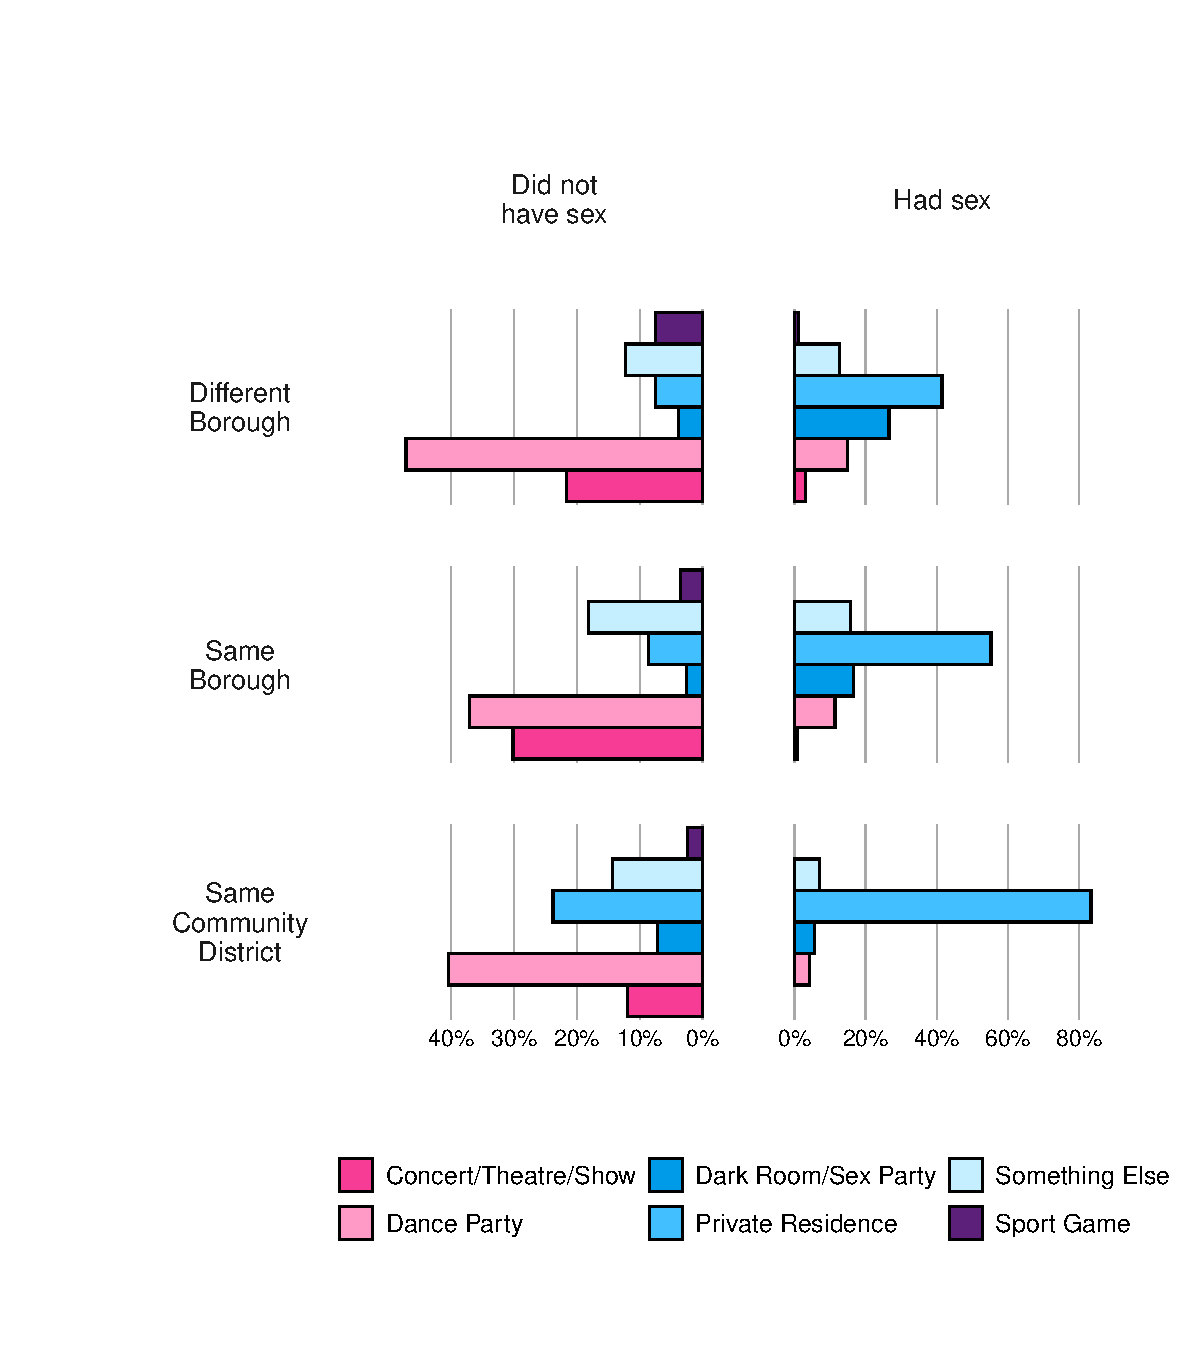
\includegraphics{3_results/3_2__results_contact_venues_files/figure-pdf/fig-placetype-bar-grid-1.pdf}

}

\caption{\label{fig-placetype-bar-grid}MPX NYC contact venue type by
distance from home and sexual contact}

\end{figure}

Of the \(604\) locations at which participant had physical or sexual
contact in a group setting (contact venues), about two out of five were
private residences, and about a quarter were dance parties. More than
half of the contact venues were in Manhattan, while less than a third
were in the Brooklyn. A quarter of all contact venues were in the same
community as the participant's residence, a third were in a different
borough, and the remainder were in the same borough as home, but a
different community district.

\begin{Shaded}
\begin{Highlighting}[]
\FunctionTok{make\_tabledata\_places}\NormalTok{() }\SpecialCharTok{|\textgreater{}}
        \FunctionTok{draw\_table\_by\_placeSex}\NormalTok{()}
\end{Highlighting}
\end{Shaded}

\hypertarget{tbl-places-descriptives}{}
\setlength{\LTpost}{0mm}
\begin{longtable}{lcccc}
\caption{\label{tbl-places-descriptives}Contact venue by venue and contact type }\tabularnewline

\toprule
 & \multicolumn{3}{c}{\textbf{Physical or sexual contact in group setting in past 4 weeks}} &  \\ 
\cmidrule(lr){2-4}
\textbf{Variable} & \textbf{Did not have sex}\\
N = 264\textsuperscript{\textit{1}} & \textbf{Had sex}\\
N = 352\textsuperscript{\textit{1}} & \textbf{Overall}\\
N = 616\textsuperscript{\textit{1}} & \textbf{p-value}\textsuperscript{\textit{2}} \\ 
\midrule\addlinespace[2.5pt]
\textbf{Place type} &  &  &  & <.001 \\ 
    Concert/Theatre/Show & 63 (24\%) & 4 (1.1\%) & 67 (11\%) &  \\ 
    Dance Party & 110 (42\%) & 33 (9.4\%) & 143 (23\%) &  \\ 
    Dark Room/Sex Party & 10 (3.8\%) & 52 (15\%) & 62 (10\%) &  \\ 
    Private Residence & 28 (11\%) & 222 (63\%) & 250 (41\%) &  \\ 
    Something Else & 40 (15\%) & 40 (11\%) & 80 (13\%) &  \\ 
    Sport Game & 13 (4.9\%) & 1 (0.3\%) & 14 (2.3\%) &  \\ 
\textbf{Place borough} &  &  &  & 0.3 \\ 
    Bronx & 6 (2.3\%) & 18 (5.1\%) & 24 (3.9\%) &  \\ 
    Brooklyn & 84 (32\%) & 96 (27\%) & 180 (29\%) &  \\ 
    Manhattan & 144 (55\%) & 188 (53\%) & 332 (54\%) &  \\ 
    Queens & 29 (11\%) & 48 (14\%) & 77 (13\%) &  \\ 
    Staten Island & 1 (0.4\%) & 2 (0.6\%) & 3 (0.5\%) &  \\ 
\textbf{Distance from home} &  &  &  & <.001 \\ 
    Same Community District & 42 (16\%) & 144 (41\%) & 186 (30\%) &  \\ 
    Same Borough & 116 (44\%) & 114 (32\%) & 230 (37\%) &  \\ 
    Different Borough & 106 (40\%) & 94 (27\%) & 200 (32\%) &  \\ 
\bottomrule
\end{longtable}
\begin{minipage}{\linewidth}
\textsuperscript{\textit{1}}n (\%)\\
\textsuperscript{\textit{2}}Pearson's Chi-squared test; Fisher's exact test\\
\emph{Data source: MPX NYC 2022}\\
\end{minipage}

Contact venues at which participants had sexual contact (rather than
non-sexual physical contact) were overwhelmingly private residences
whereas contact venues at which they had non-sexual physical contact
were mostly dance parties (see Figure~\ref{fig-placetype-bar-grid}). The
closer to home a location was, the more likely it was to be a private
residence and the more likely it was the site of sexual contact. By
contrast, the further from home a contact venue was, the more likely it
was to be a dance party.

\begin{Shaded}
\begin{Highlighting}[]
\FunctionTok{plot\_icon}\NormalTok{(}\AttributeTok{icon\_name =} \StringTok{"taco"}\NormalTok{, }\AttributeTok{color =} \StringTok{"dark\_green"}\NormalTok{, }\AttributeTok{shape =} \DecValTok{4}\NormalTok{)}
\end{Highlighting}
\end{Shaded}

\begin{figure}[H]

{\centering 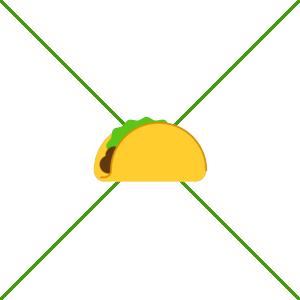
\includegraphics{3_results/3_2__results_contact_venues_files/figure-pdf/unnamed-chunk-4-1.pdf}

}

\end{figure}

\hypertarget{sec-movement}{%
\chapter{Movement}\label{sec-movement}}

\begin{Shaded}
\begin{Highlighting}[]
\CommentTok{\# Access custom defined functions}
\NormalTok{targets}\SpecialCharTok{::}\FunctionTok{tar\_source}\NormalTok{(}\StringTok{"../R\_functions"}\NormalTok{)}
\end{Highlighting}
\end{Shaded}

\hypertarget{spatial-patterns}{%
\section{Spatial patterns}\label{spatial-patterns}}

Figure~\ref{fig-movement-matrix} maps each contact venue's community
district (x-axis) against the participant's home community district
(y-axis). The size of the dot is proportional to the total count of
contact venues with the given home and contact venue community district.
The color of the dot represents the borough of the contact venue.

The dots on the diagonal line from top left to bottom right, show
prominently, indicating that a sizeable proportion of movement happens
within community districts. The figure also shows four prominent
clusters - the cluster at the top left (in pink) shows significant
movement between home and contact venues within Brooklyn and the cluster
towards the middle of the plot (in purple) shows significant movement
within Manhattan. The clusters at the top center and bottom left show
significant movement from Brooklyn to Manhattan and from Manhattan to
Brooklyn, respectively.

\begin{Shaded}
\begin{Highlighting}[]
\FunctionTok{make\_plotdata\_movement\_matrix}\NormalTok{() }\SpecialCharTok{|\textgreater{}}
  \FunctionTok{plot\_matrix\_movement}\NormalTok{() }\SpecialCharTok{+}
  \FunctionTok{theme\_mpxnyc\_blank}\NormalTok{() }\SpecialCharTok{+}
  \FunctionTok{scale\_fill\_mpxnyc}\NormalTok{(}\AttributeTok{name =} \StringTok{"From Borough"}\NormalTok{, }\AttributeTok{option =} \StringTok{"dark"}\NormalTok{) }\SpecialCharTok{+}
  \FunctionTok{scale\_color\_mpxnyc}\NormalTok{(}\AttributeTok{name =} \StringTok{"To Borough"}\NormalTok{, }\AttributeTok{option =} \StringTok{"dark"}\NormalTok{) }\SpecialCharTok{+}
\NormalTok{  ggplot2}\SpecialCharTok{::}\FunctionTok{scale\_size\_continuous}\NormalTok{(}\AttributeTok{name =} \StringTok{"Count"}\NormalTok{) }\SpecialCharTok{+}
  \FunctionTok{theme\_mpxnyc\_matrix\_movement}\NormalTok{() }
\end{Highlighting}
\end{Shaded}

\begin{figure}[H]

{\centering 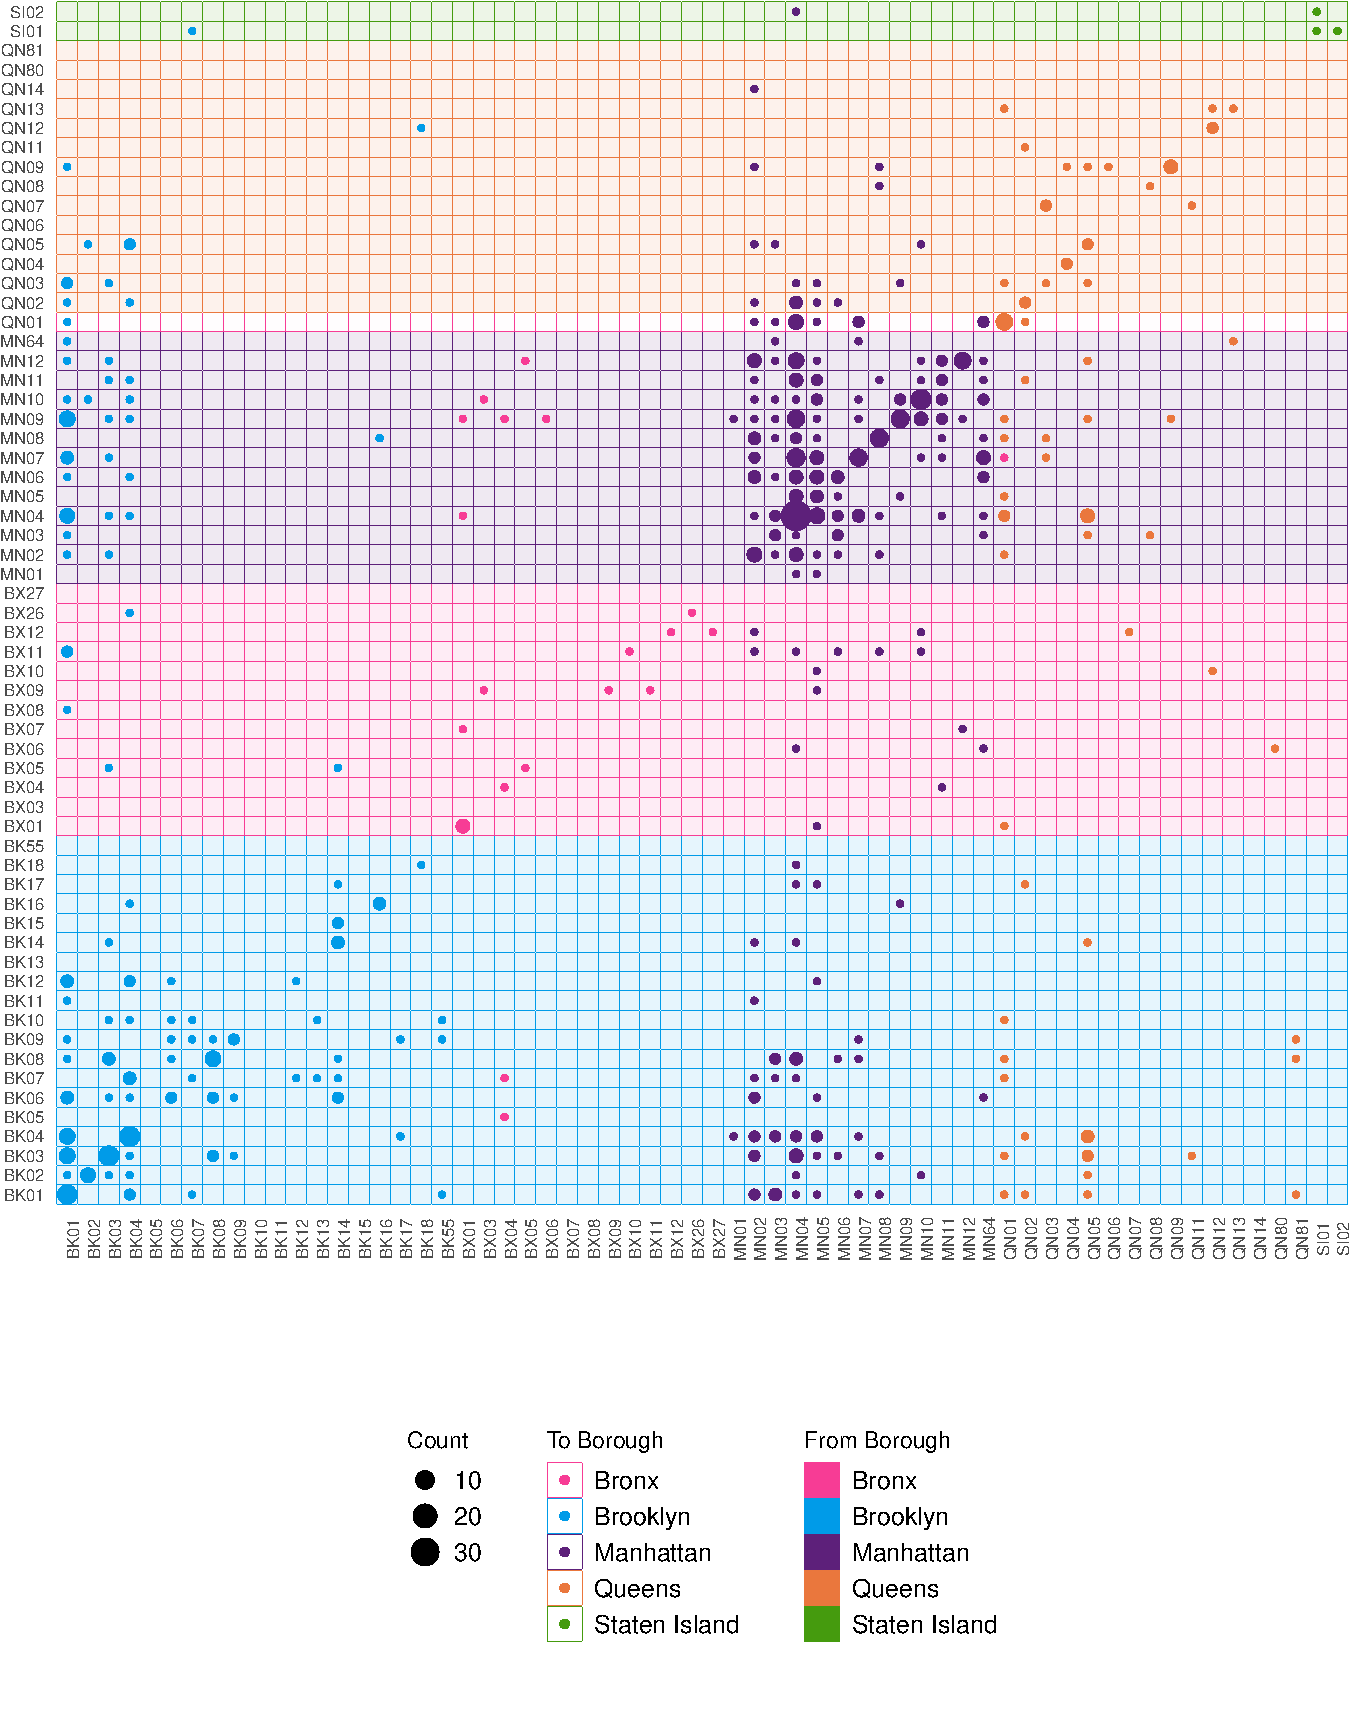
\includegraphics{3_results/3_3__results_movement_files/figure-pdf/fig-movement-matrix-1.pdf}

}

\caption{\label{fig-movement-matrix}Movement between home and contact
venues by MPX NYC participant. The figure maps each contact venue's
community district (x-axis) against the participant's home community
district (y-axis). The size of the dot is proportional to the total
count of contact venues with the given home and contact venue community
district. The color of the dot represents the borough of the contact
venue.}

\end{figure}

\hypertarget{spatial-concentration}{%
\section{Spatial concentration}\label{spatial-concentration}}

Figure~\ref{fig-spatial-concentration-bar} shows the difference betweeen
the proportion of primary residences in each community district and the
proprotion of contact venues in each community district. It shows that
within Brooklyn, Manhattan, and Queens, there is a small set of
community districts which tend to be markedly over-represented among
contact venues compared to their share of primary residences. These are
BK01, MN05, and QN05, respectively.

\begin{Shaded}
\begin{Highlighting}[]
\FunctionTok{make\_plotdata\_spatial\_concentration\_bar}\NormalTok{() }\SpecialCharTok{|\textgreater{}}
  \FunctionTok{plot\_home\_vs\_residence\_dbn\_bar}\NormalTok{() }\SpecialCharTok{+}
\NormalTok{  ggplot2}\SpecialCharTok{::}\FunctionTok{coord\_flip}\NormalTok{() }\SpecialCharTok{+}
  \FunctionTok{scale\_fill\_mpxnyc}\NormalTok{(}\AttributeTok{name =} \StringTok{"Borough"}\NormalTok{, }\AttributeTok{option =} \StringTok{"dark"}\NormalTok{) }\SpecialCharTok{+}
\NormalTok{  ggplot2}\SpecialCharTok{::}\FunctionTok{scale\_alpha\_manual}\NormalTok{(}\AttributeTok{values =} \FunctionTok{c}\NormalTok{(}\StringTok{"highlight"} \OtherTok{=} \DecValTok{1}\NormalTok{, }\StringTok{"lowlight"} \OtherTok{=} \FloatTok{0.5}\NormalTok{), }\AttributeTok{guide=}\StringTok{"none"}\NormalTok{) }\SpecialCharTok{+}
\NormalTok{  ggplot2}\SpecialCharTok{::}\FunctionTok{scale\_y\_continuous}\NormalTok{(}\AttributeTok{labels =}\NormalTok{ scales}\SpecialCharTok{::}\FunctionTok{percent\_format}\NormalTok{(}\AttributeTok{scale =} \DecValTok{100}\NormalTok{)) }\SpecialCharTok{+}
  \FunctionTok{theme\_mpxnyc\_home\_vs\_place}\NormalTok{() }
\end{Highlighting}
\end{Shaded}

\begin{figure}[H]

{\centering 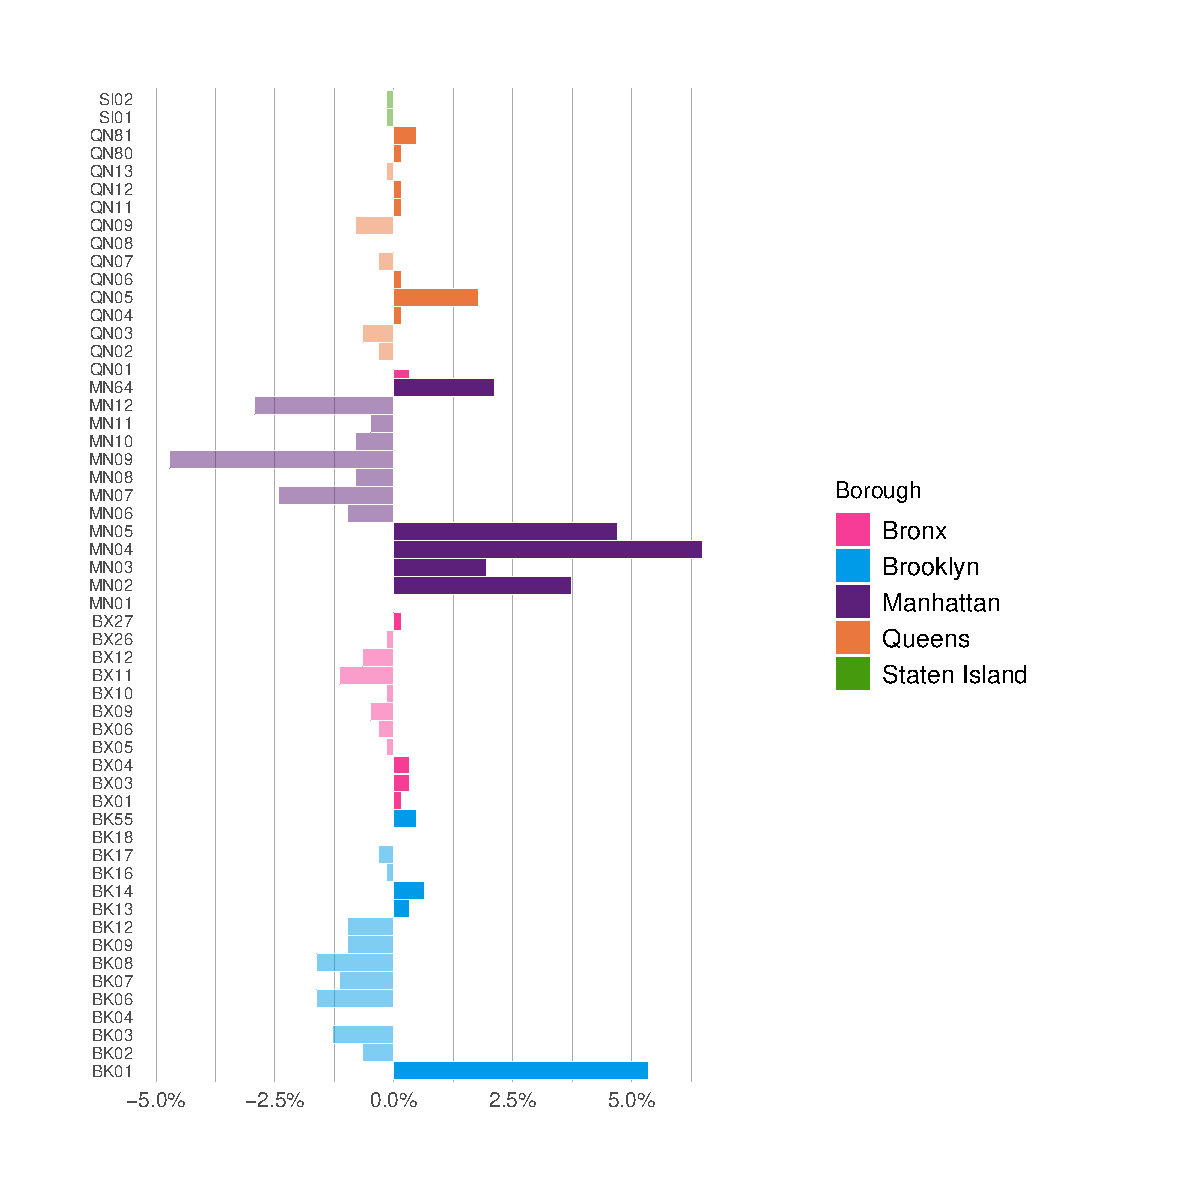
\includegraphics{3_results/3_3__results_movement_files/figure-pdf/fig-spatial-concentration-bar-1.pdf}

}

\caption{\label{fig-spatial-concentration-bar}Overall Movement between
home and contact venues by MPX NYC participant. The figure shows each
community districts over-representation among contact venues compared to
residences}

\end{figure}

\begin{Shaded}
\begin{Highlighting}[]
\FunctionTok{plot\_icon}\NormalTok{(}\AttributeTok{icon\_name =} \StringTok{"eggplant"}\NormalTok{, }\AttributeTok{color =} \StringTok{"dark\_green"}\NormalTok{, }\AttributeTok{shape =} \DecValTok{8}\NormalTok{)}
\end{Highlighting}
\end{Shaded}

\begin{figure}[H]

{\centering 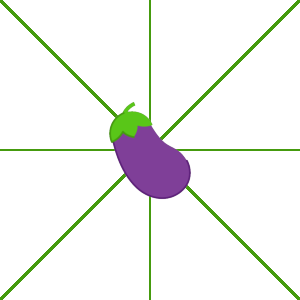
\includegraphics{3_results/3_3__results_movement_files/figure-pdf/unnamed-chunk-4-1.pdf}

}

\end{figure}

\hypertarget{mixing}{%
\chapter{Mixing}\label{mixing}}

\begin{Shaded}
\begin{Highlighting}[]
\CommentTok{\# Access custom defined functions}
\NormalTok{targets}\SpecialCharTok{::}\FunctionTok{tar\_source}\NormalTok{(}\StringTok{"../R\_functions"}\NormalTok{)}
\end{Highlighting}
\end{Shaded}

The figures in this section quantify the degree to which individuals
with characteristics shown on the left live or play in an overlapping
set of community districts with individuals whose characteristics are
shown at the top.

Overall, MPX NYC participants showed spatial homophily - the spatial
selection coefficient from a given group to the same group was positive
for all levels of race-gender, sexual orientation, and age. In addition,
black cisgender men and non-binary persons tended to visit or live in
different neighborhoods than white cisgender men. Non-binary persons
also showed a preference for community districts in which transgender
men live. Gay identified participants preferred to live and play in
community districts where bisexual, straight and queer identified
participants did not live. Similarly, those groups selected against
community districts in which gay identified individuals live or play.

\hypertarget{race-and-gender}{%
\section{Race and gender}\label{race-and-gender}}

\begin{Shaded}
\begin{Highlighting}[]
\FunctionTok{make\_plotdata\_racegender\_mixing\_matrix}\NormalTok{() }\SpecialCharTok{|\textgreater{}}
  \FunctionTok{plot\_matrix\_mixing}\NormalTok{() }\SpecialCharTok{+}
  \FunctionTok{scale\_fill\_mpxnyc\_gradient}\NormalTok{() }\SpecialCharTok{+}
  \FunctionTok{scale\_color\_mpxnyc\_gradient}\NormalTok{() }\SpecialCharTok{+}
  \FunctionTok{theme\_mpxnyc\_mixing}\NormalTok{()}
\end{Highlighting}
\end{Shaded}

\begin{figure}[H]

{\centering 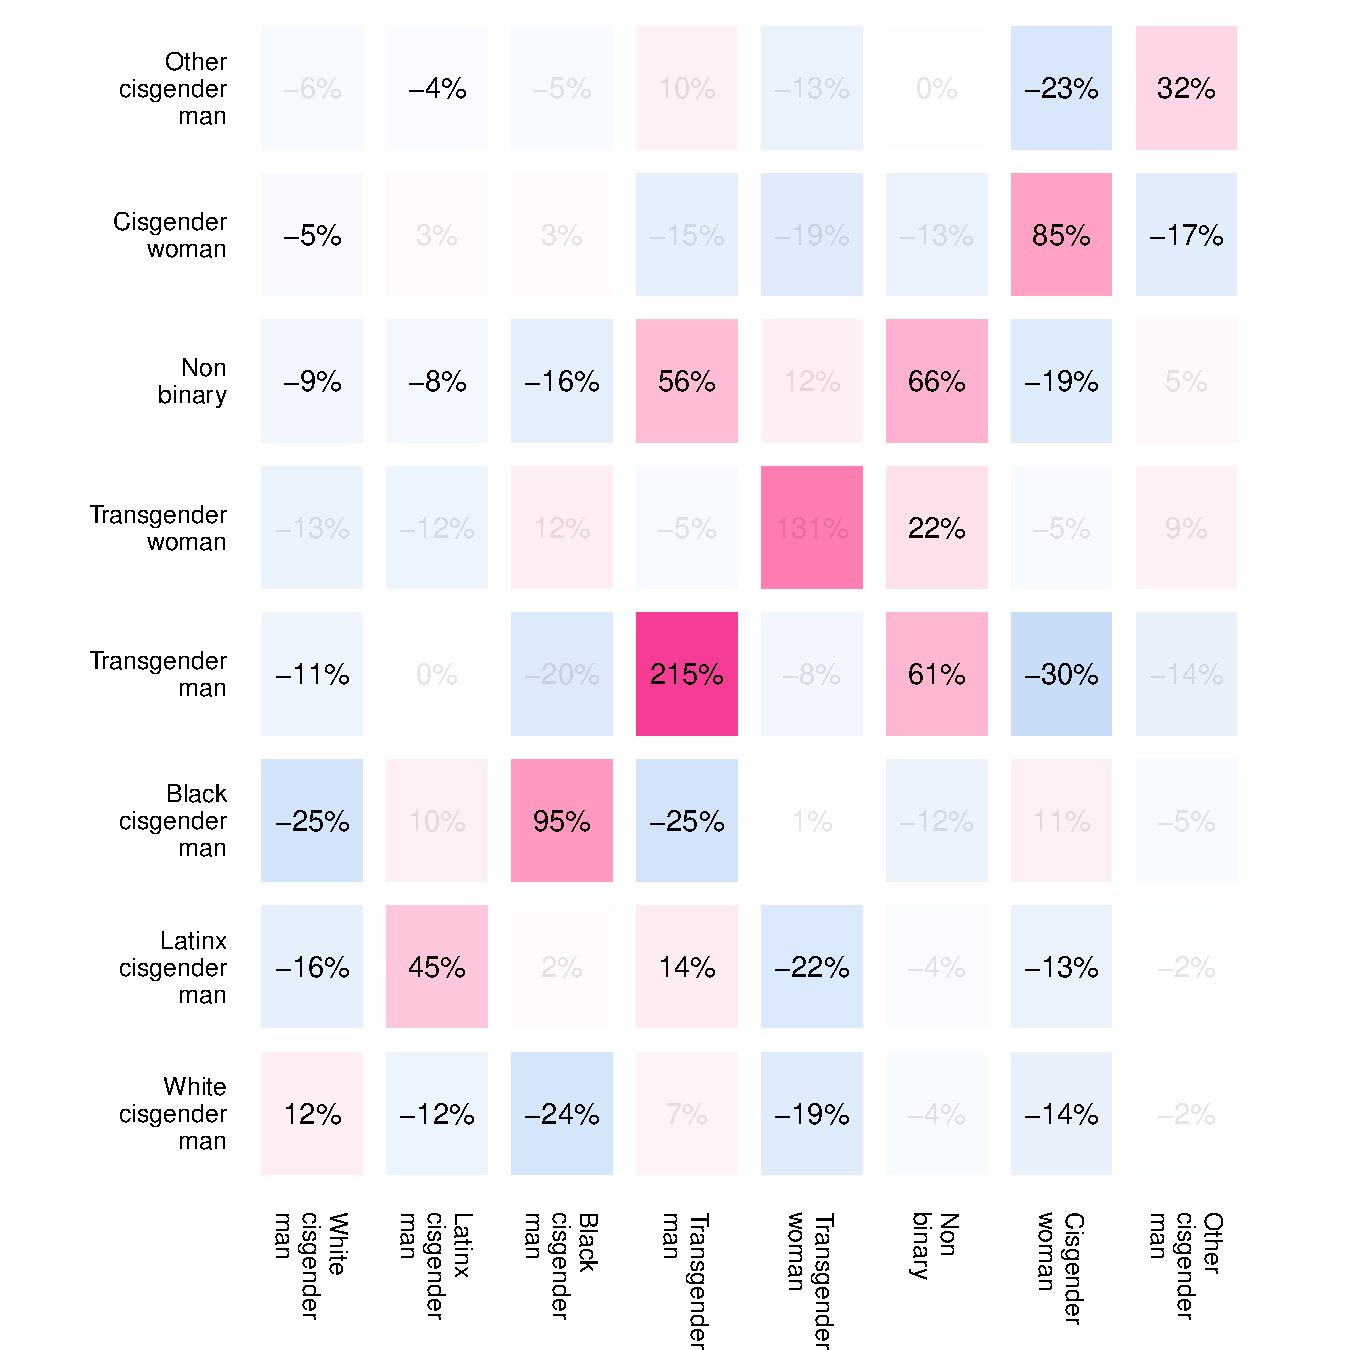
\includegraphics{3_results/3_4__results_mixing_files/figure-pdf/fig-racegender-mixing-matrix-1.pdf}

}

\caption{\label{fig-racegender-mixing-matrix}Social mixing matrices for
MPX NYC participants by race-gende}

\end{figure}

\hypertarget{sexual-orientation}{%
\section{Sexual orientation}\label{sexual-orientation}}

\begin{Shaded}
\begin{Highlighting}[]
\FunctionTok{make\_plotdata\_sexorientation\_mixing\_matrix}\NormalTok{() }\SpecialCharTok{|\textgreater{}}
  \FunctionTok{plot\_matrix\_mixing}\NormalTok{() }\SpecialCharTok{+}
  \FunctionTok{scale\_fill\_mpxnyc\_gradient}\NormalTok{() }\SpecialCharTok{+}
  \FunctionTok{scale\_color\_mpxnyc\_gradient}\NormalTok{() }\SpecialCharTok{+}
  \FunctionTok{theme\_mpxnyc\_mixing}\NormalTok{() }\SpecialCharTok{+}
\NormalTok{  ggplot2}\SpecialCharTok{::}\FunctionTok{theme}\NormalTok{(}
    \AttributeTok{plot.margin =}\NormalTok{ ggplot2}\SpecialCharTok{::}\FunctionTok{unit}\NormalTok{(}\DecValTok{10}\SpecialCharTok{*}\FunctionTok{c}\NormalTok{(}\DecValTok{10}\NormalTok{,}\DecValTok{10}\NormalTok{,}\DecValTok{10}\NormalTok{,}\DecValTok{10}\NormalTok{), }\StringTok{"pt"}\NormalTok{)}
\NormalTok{    )}
\end{Highlighting}
\end{Shaded}

\begin{figure}[H]

{\centering 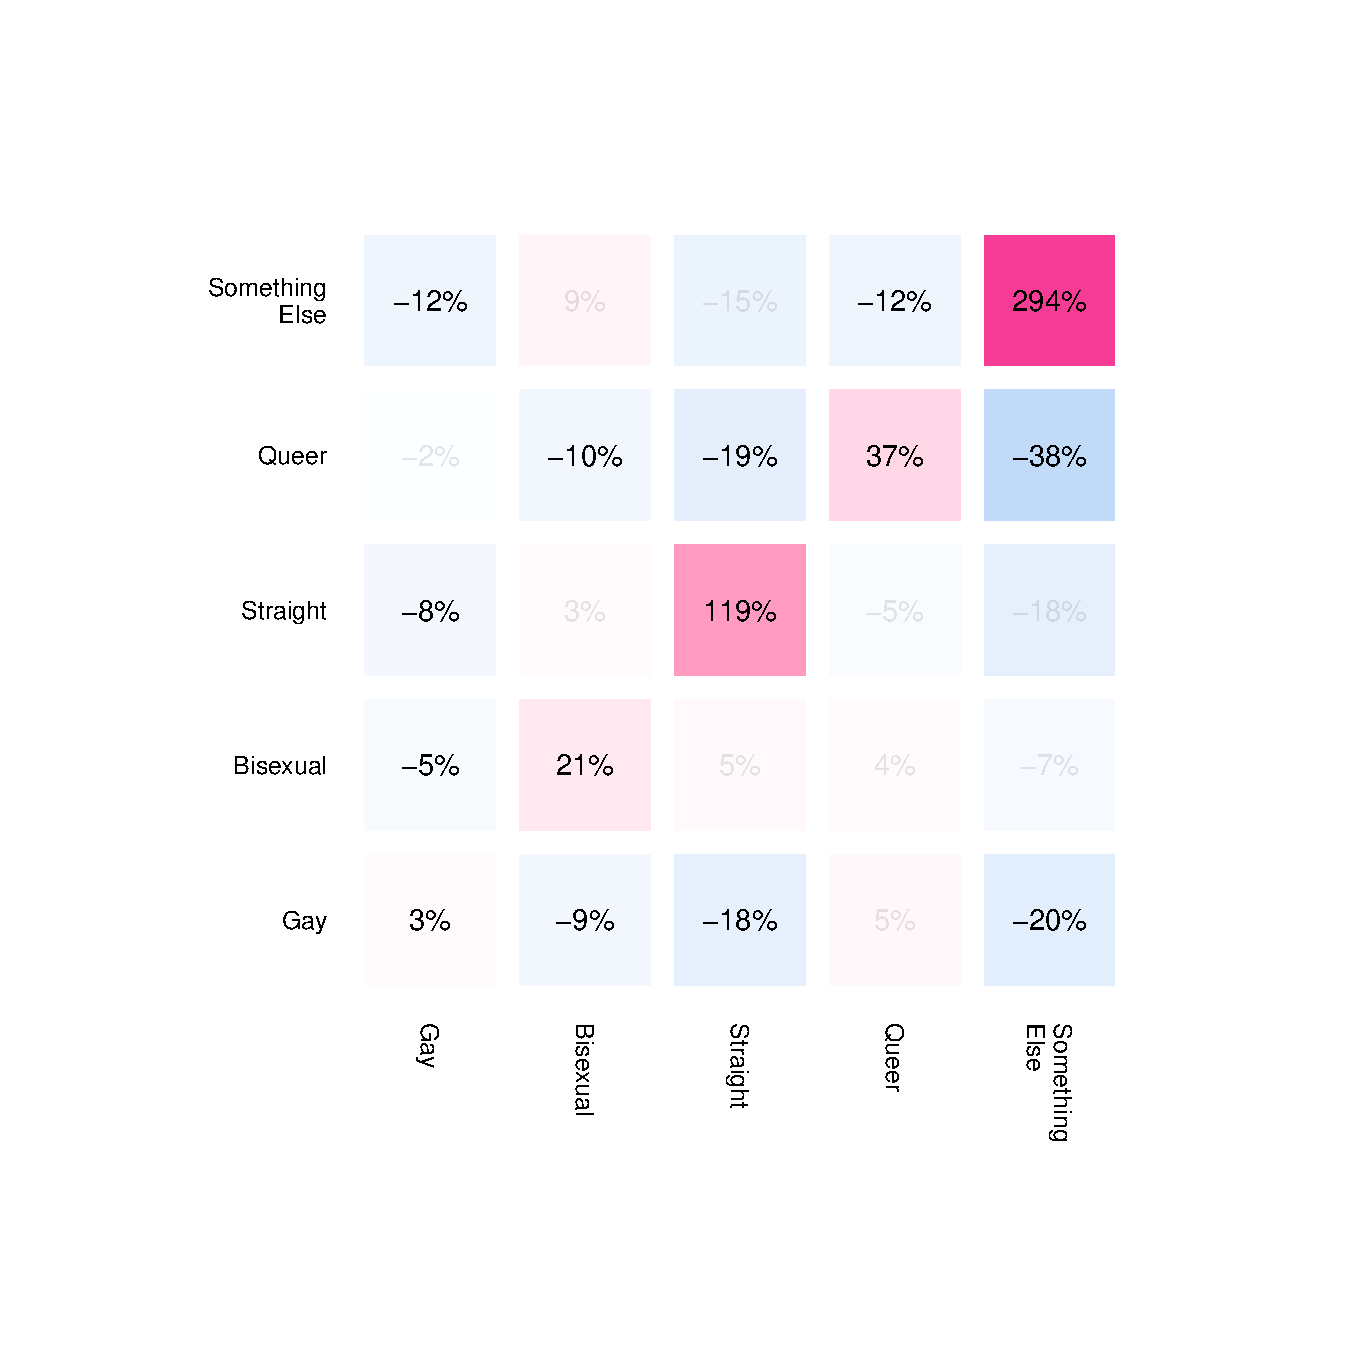
\includegraphics{3_results/3_4__results_mixing_files/figure-pdf/fig-sexorientation-mixing-matrix-1.pdf}

}

\caption{\label{fig-sexorientation-mixing-matrix}Social mixing matrix
for MPX NYC participants by sexual orientation}

\end{figure}

\hypertarget{age}{%
\section{Age}\label{age}}

\begin{Shaded}
\begin{Highlighting}[]
\FunctionTok{make\_plotdata\_age\_mixing\_matrix}\NormalTok{() }\SpecialCharTok{|\textgreater{}}
  \FunctionTok{plot\_matrix\_mixing}\NormalTok{() }\SpecialCharTok{+}
  \FunctionTok{scale\_fill\_mpxnyc\_gradient}\NormalTok{() }\SpecialCharTok{+}
  \FunctionTok{scale\_color\_mpxnyc\_gradient}\NormalTok{() }\SpecialCharTok{+}
  \FunctionTok{theme\_mpxnyc\_mixing}\NormalTok{() }\SpecialCharTok{+}
\NormalTok{  ggplot2}\SpecialCharTok{::}\FunctionTok{theme}\NormalTok{(}
    \AttributeTok{plot.margin =}\NormalTok{ ggplot2}\SpecialCharTok{::}\FunctionTok{unit}\NormalTok{(}\DecValTok{10}\SpecialCharTok{*}\FunctionTok{c}\NormalTok{(}\DecValTok{10}\NormalTok{,}\DecValTok{10}\NormalTok{,}\DecValTok{10}\NormalTok{,}\DecValTok{10}\NormalTok{), }\StringTok{"pt"}\NormalTok{)}
\NormalTok{  )}
\end{Highlighting}
\end{Shaded}

\begin{figure}[H]

{\centering 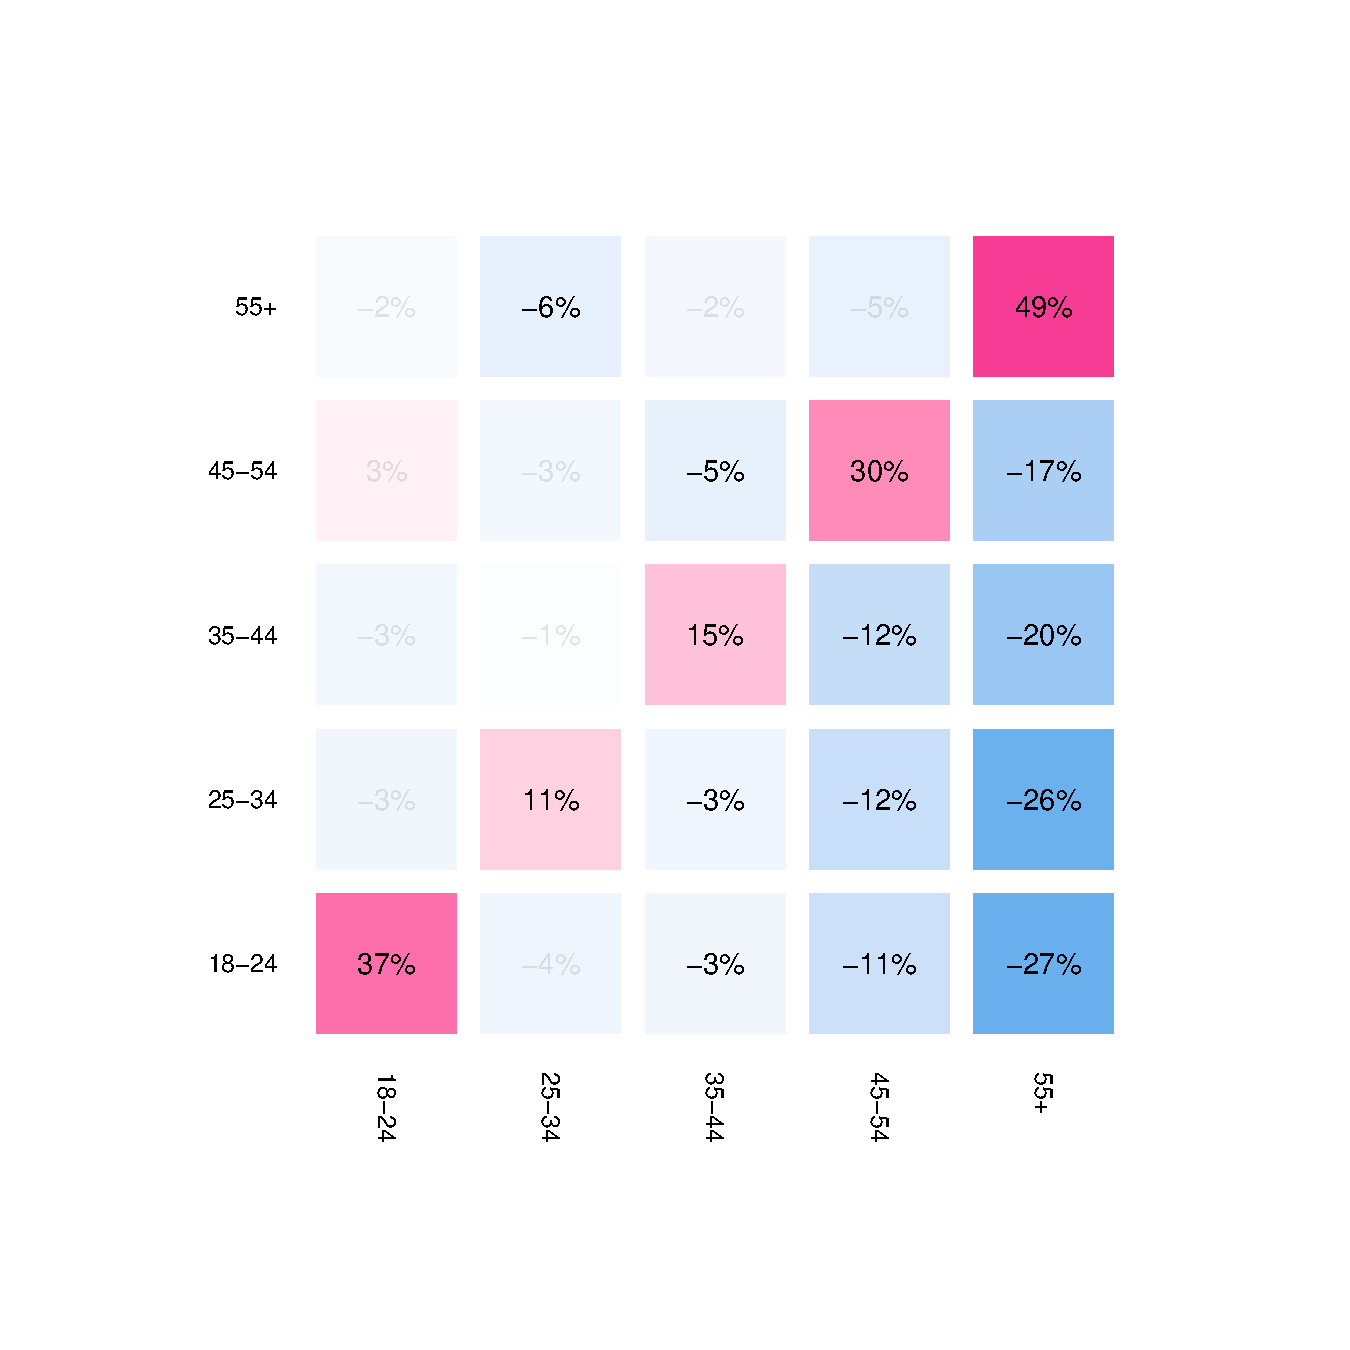
\includegraphics{3_results/3_4__results_mixing_files/figure-pdf/fig-age-mixing-matrix-1.pdf}

}

\caption{\label{fig-age-mixing-matrix}Social mixing matrix for MPX NYC
participants by age}

\end{figure}

\begin{Shaded}
\begin{Highlighting}[]
\FunctionTok{plot\_icon}\NormalTok{(}\AttributeTok{icon\_name =} \StringTok{"bear"}\NormalTok{, }\AttributeTok{color =} \StringTok{"light\_brown"}\NormalTok{, }\AttributeTok{shape =} \DecValTok{8}\NormalTok{)}
\end{Highlighting}
\end{Shaded}

\begin{figure}[H]

{\centering 
\includegraphics{3_results/3_4__results_mixing_files/figure-pdf/unnamed-chunk-5-1.pdf}

}

\end{figure}

\hypertarget{sec-intervention}{%
\chapter{Outbreak control}\label{sec-intervention}}

\begin{Shaded}
\begin{Highlighting}[]
\CommentTok{\# Access custom defined functions}
\NormalTok{targets}\SpecialCharTok{::}\FunctionTok{tar\_source}\NormalTok{(}\StringTok{"../R\_functions"}\NormalTok{)}
\end{Highlighting}
\end{Shaded}

\begin{Shaded}
\begin{Highlighting}[]
\FunctionTok{make\_plotdata\_coverage\_approach\_choro}\NormalTok{() }\SpecialCharTok{|\textgreater{}}
                \FunctionTok{plot\_coverage\_map}\NormalTok{()  }\SpecialCharTok{+}
                \FunctionTok{scale\_fill\_mpxnyc}\NormalTok{(}\AttributeTok{name =} \StringTok{""}\NormalTok{, }\AttributeTok{na.translate =} \ConstantTok{FALSE}\NormalTok{, }\AttributeTok{option =} \StringTok{"light"}\NormalTok{) }\SpecialCharTok{+}
                \FunctionTok{theme\_mpxnyc\_blank}\NormalTok{() }\SpecialCharTok{+}
\NormalTok{                ggplot2}\SpecialCharTok{::}\FunctionTok{theme}\NormalTok{(}\AttributeTok{legend.position =} \StringTok{"bottom"}\NormalTok{)}
\end{Highlighting}
\end{Shaded}

\begin{figure}[H]

{\centering 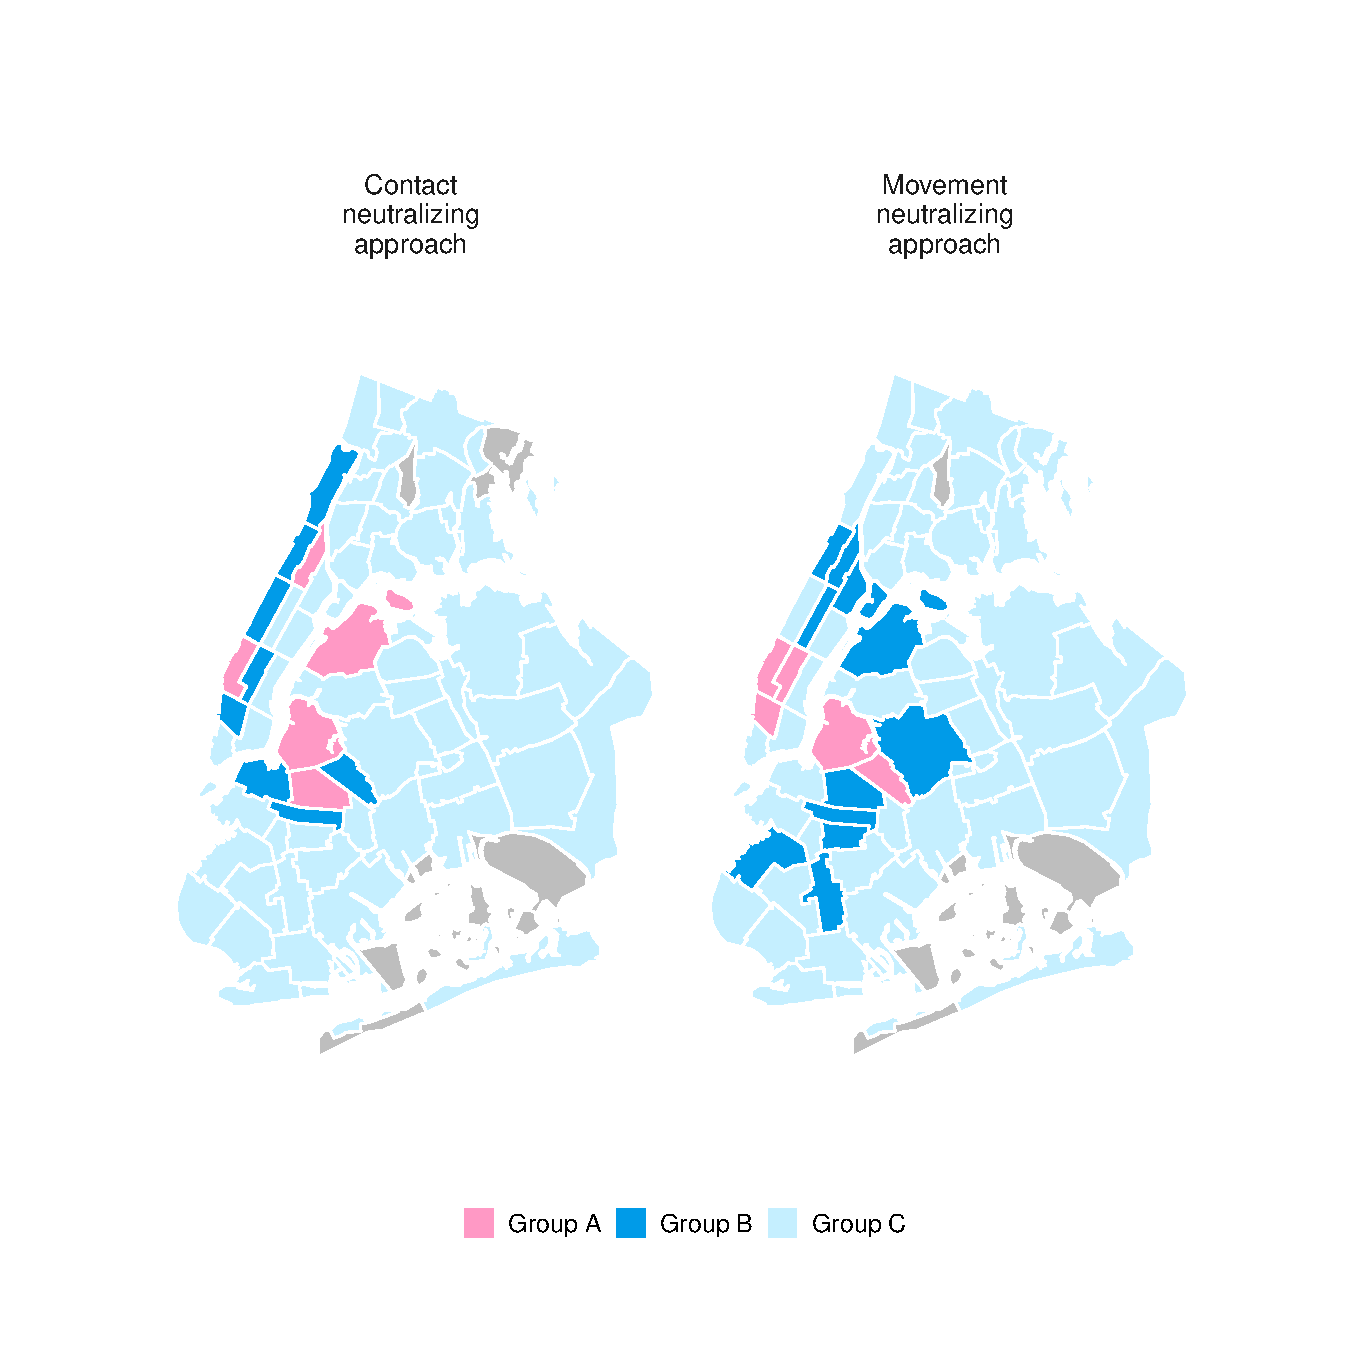
\includegraphics{3_results/3_5__results_outbreak_control_files/figure-pdf/fig-hiimpact-communities-map-1.pdf}

}

\caption{\label{fig-hiimpact-communities-map}High-coverage community
districts: contact vs movement-neutralizing strategy}

\end{figure}

\hypertarget{spatial-efficiency-1}{%
\section{Spatial efficiency}\label{spatial-efficiency-1}}

\begin{Shaded}
\begin{Highlighting}[]
\FunctionTok{make\_plotdata\_coverage\_approach\_bar}\NormalTok{() }\SpecialCharTok{|\textgreater{}}
  \FunctionTok{plot\_coverage\_bar}\NormalTok{() }\SpecialCharTok{+}
  \FunctionTok{scale\_fill\_mpxnyc}\NormalTok{(}\AttributeTok{name =} \StringTok{""}\NormalTok{, }\AttributeTok{na.translate =} \ConstantTok{FALSE}\NormalTok{, }\AttributeTok{option =} \StringTok{"light"}\NormalTok{)  }\SpecialCharTok{+}
  \FunctionTok{theme\_mpxnyc\_blank}\NormalTok{() }\SpecialCharTok{+}
\NormalTok{  ggplot2}\SpecialCharTok{::}\FunctionTok{theme}\NormalTok{(}\AttributeTok{legend.position =} \StringTok{"bottom"}\NormalTok{) }
\end{Highlighting}
\end{Shaded}

\begin{figure}[H]

{\centering 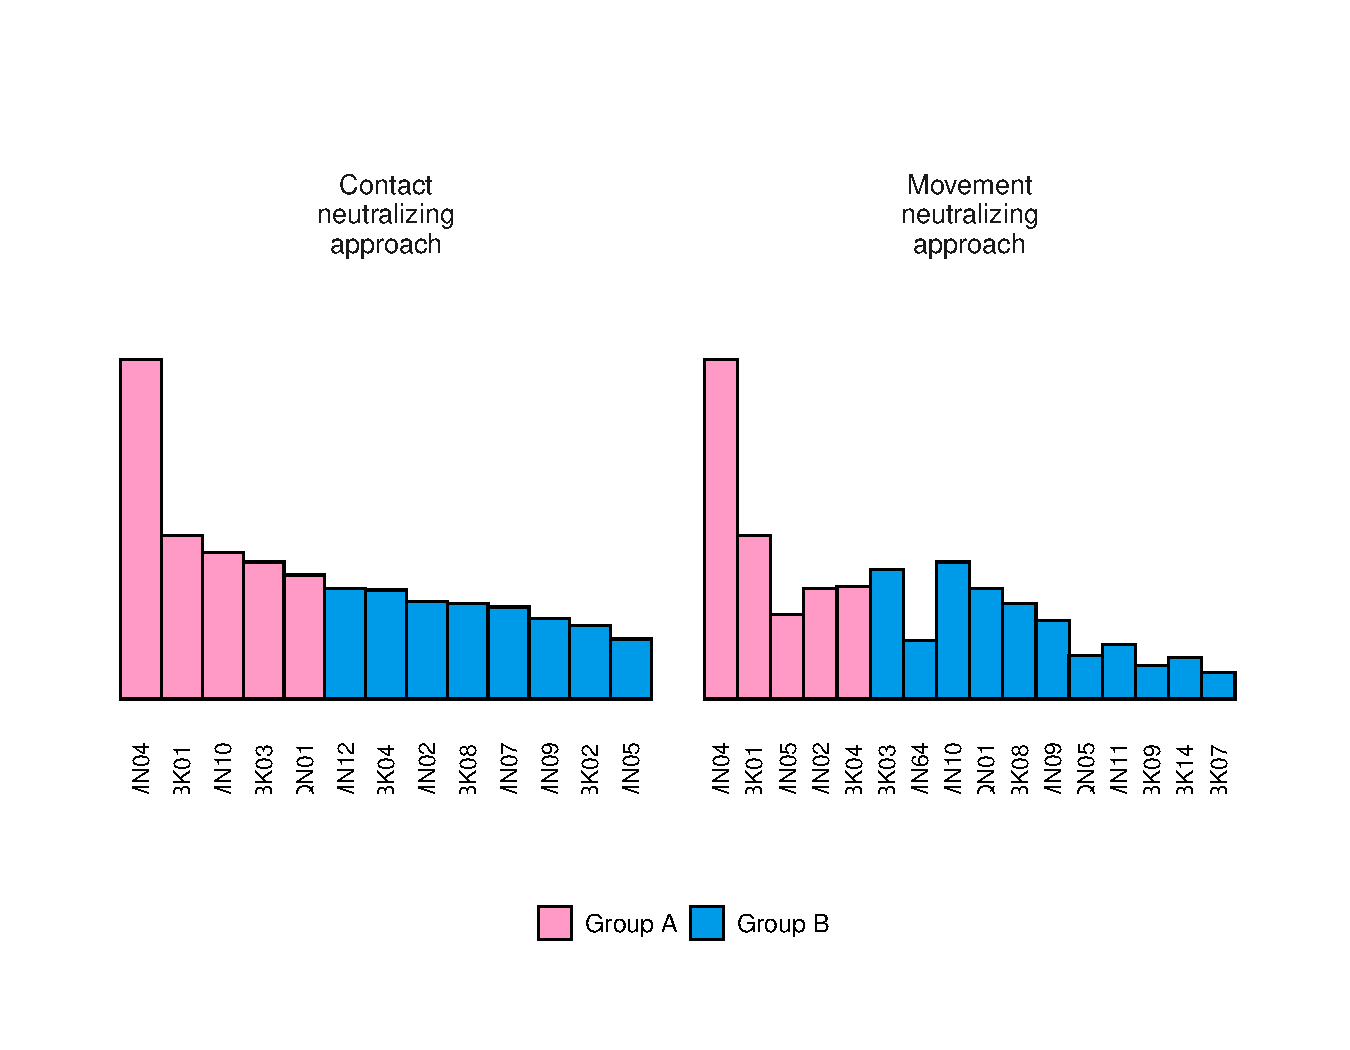
\includegraphics{3_results/3_5__results_outbreak_control_files/figure-pdf/fig-hiimpact-communities-bar-1.pdf}

}

\caption{\label{fig-hiimpact-communities-bar}High-coverage community
districts: contact vs movement-neutralizing strategy}

\end{figure}

Figure~\ref{fig-hiimpact-communities-bar} and
Figure~\ref{fig-hiimpact-communities-map} show which community districts
would have to be immunized to immunize 33\% of the population (Group A),
and 66\% of the population (Group A + Group B) under both the
contact-neutralizing and movement-neutralizing intervention strategies.

Under the contact-neutralizing strategy, it would take five community
districts to immunize 33\% of the population. These are MN04, BK01,
MN10, BK03, and QN01. To reach 66\% of participants with the
intervention, it would be necessary to immunize 13 community districts.
The additional community districts would be MN12, BK04, MN02, BK08,
MN07, MN09, BK02, and MN05.

Under the movement-neutralizing strategy, it would take six community
districts to reach 33\% of the population: MN04, BK01, MN05, BK04, MN02,
and BK03. It would take 16 community districts to reach 66\% of the
population. The additional community districts would be: MN64, MN10,
QN01, BK08, MN09, QN05, BK09, MN11, BK14, and BK07.

\hypertarget{network-impact}{%
\section{Network impact}\label{network-impact}}

Figure~\ref{fig-netimpact} shows that nearly 100\% of individuals are
included in the largest connected component before any intervention. For
the movement-neutralizing strategy, the proportion of the population
included in the largest connected component declines more sharply than
for the contact-neutralizing strategy as more community districts are
immunized. In the contact-neutralizing strategy, the overall proportion
of unvaccinated individuals declines more sharply than in the
movement-neutralizing strategy. There is not a noticeable difference
between the two strategies for the first 10 community districts to be
immunized - differences between the two strategies start emerging once
10 community districts are immunized.

\begin{Shaded}
\begin{Highlighting}[]
\FunctionTok{make\_plotdata\_net\_impact\_profile}\NormalTok{() }\SpecialCharTok{|\textgreater{}}
  \FunctionTok{plot\_centrality\_bar}\NormalTok{() }\SpecialCharTok{+}
  \FunctionTok{scale\_fill\_mpxnyc}\NormalTok{(}\AttributeTok{name =} \StringTok{""}\NormalTok{, }\AttributeTok{option =} \StringTok{"light"}\NormalTok{) }\SpecialCharTok{+}
\NormalTok{  ggplot2}\SpecialCharTok{::}\FunctionTok{scale\_y\_continuous}\NormalTok{(}\StringTok{"Proportion of participants"}\NormalTok{, }\AttributeTok{limits =} \FunctionTok{c}\NormalTok{(}\SpecialCharTok{{-}}\FloatTok{0.2}\NormalTok{, }\DecValTok{1}\NormalTok{), }\AttributeTok{labels =}\NormalTok{ scales}\SpecialCharTok{::}\NormalTok{percent) }\SpecialCharTok{+}
\NormalTok{  ggplot2}\SpecialCharTok{::}\FunctionTok{scale\_x\_continuous}\NormalTok{(}\StringTok{"Intervention order"}\NormalTok{, }\AttributeTok{limits =} \FunctionTok{c}\NormalTok{(}\DecValTok{0}\NormalTok{, }\DecValTok{40}\NormalTok{), }\AttributeTok{breaks =} \FunctionTok{c}\NormalTok{(}\DecValTok{0}\NormalTok{, }\DecValTok{10}\NormalTok{, }\DecValTok{20}\NormalTok{, }\DecValTok{30}\NormalTok{, }\DecValTok{40}\NormalTok{)) }\SpecialCharTok{+}
  \FunctionTok{theme\_mpxnyc\_netimpact}\NormalTok{() }
\end{Highlighting}
\end{Shaded}

\begin{figure}[H]

{\centering 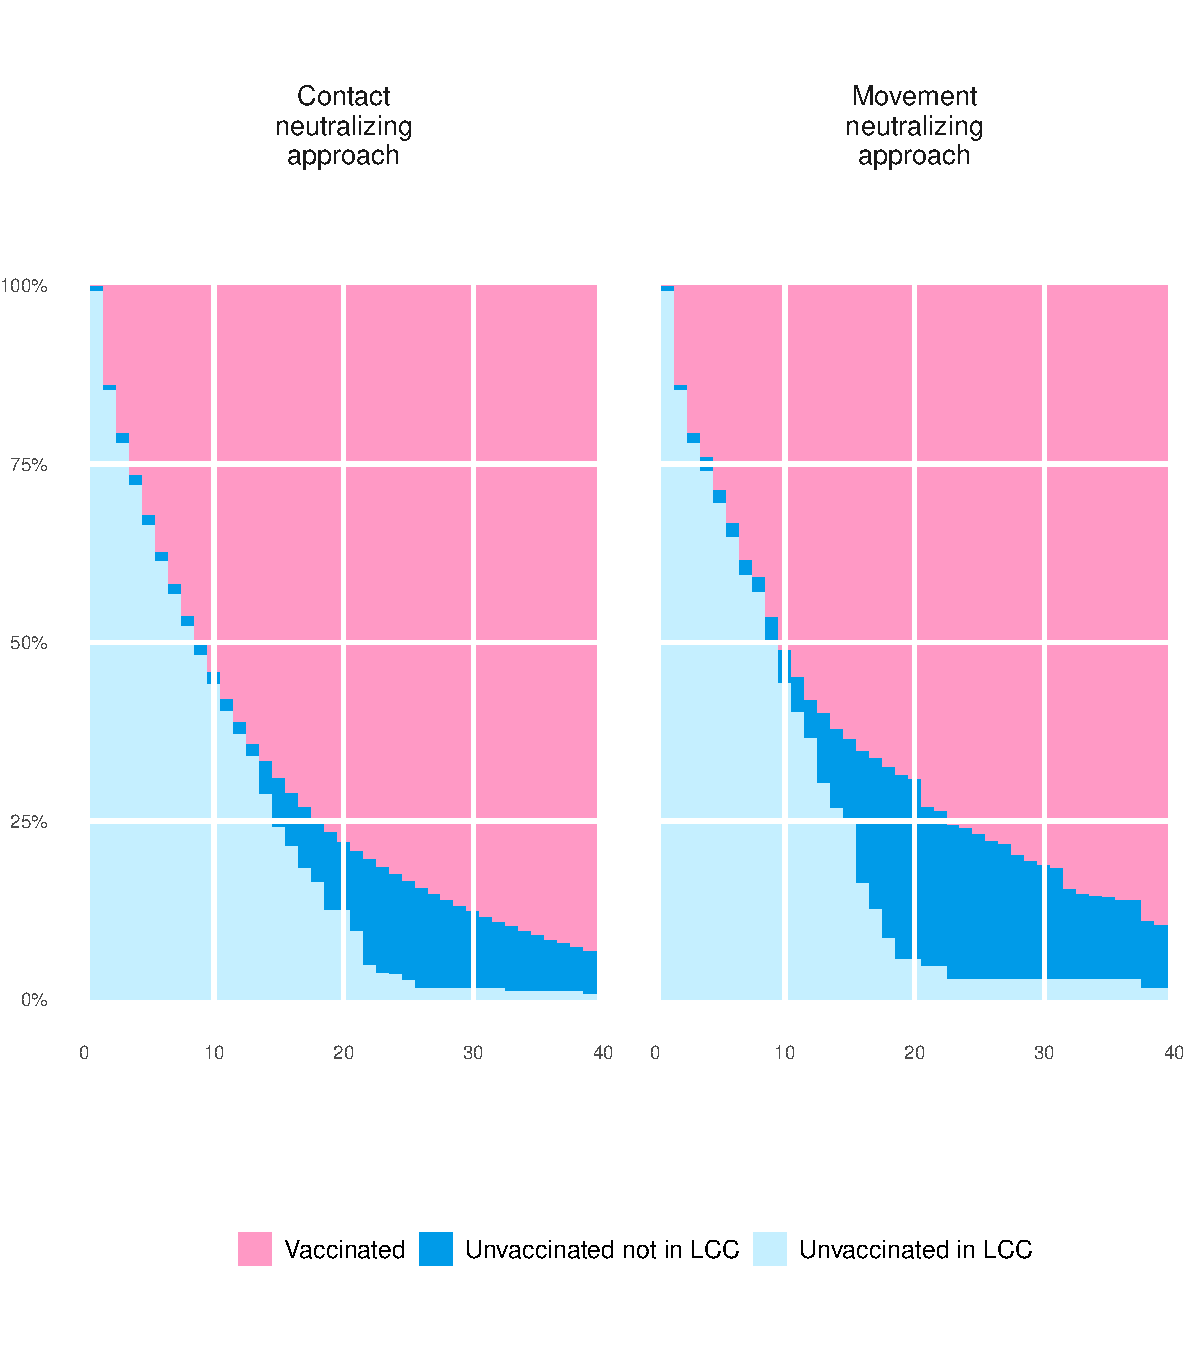
\includegraphics{3_results/3_5__results_outbreak_control_files/figure-pdf/fig-netimpact-1.pdf}

}

\caption{\label{fig-netimpact}Network impact}

\end{figure}

\begin{Shaded}
\begin{Highlighting}[]
\FunctionTok{plot\_icon}\NormalTok{(}\AttributeTok{icon\_name =} \StringTok{"unicorn"}\NormalTok{, }\AttributeTok{color =} \StringTok{"light\_pink"}\NormalTok{, }\AttributeTok{shape =} \DecValTok{8}\NormalTok{)}
\end{Highlighting}
\end{Shaded}

\begin{figure}[H]

{\centering 
\includegraphics{3_results/3_5__results_outbreak_control_files/figure-pdf/unnamed-chunk-5-1.pdf}

}

\end{figure}

\part{Conclusion}

\hypertarget{sec-discussion}{%
\chapter{Discussion}\label{sec-discussion}}

\hypertarget{sec-recommendations}{%
\chapter{Recommendations}\label{sec-recommendations}}

\part{Endnotes}

\hypertarget{references}{%
\chapter{References}\label{references}}

\begin{Shaded}
\begin{Highlighting}[]
\NormalTok{targets}\SpecialCharTok{::}\FunctionTok{tar\_source}\NormalTok{(}\StringTok{"R\_functions"}\NormalTok{)}
\end{Highlighting}
\end{Shaded}

\hypertarget{refs}{}
\begin{CSLReferences}{1}{0}
\leavevmode\vadjust pre{\hypertarget{ref-annagracelee}{}}%
Anna Grace Lee. n.d. {``Will the Specter of Monkeypox Affect Pride
Weekend in New York?''} \emph{New York Times}.
\url{https://www.nytimes.com/2022/06/25/style/monkeypox-nyc-pride.html}.

\leavevmode\vadjust pre{\hypertarget{ref-aronow2017}{}}%
Aronow, Peter M, and Cyrus Samii. 2017. {``Estimating Average Causal
Effects Under General Interference, with Application to a Social Network
Experiment.''}

\leavevmode\vadjust pre{\hypertarget{ref-blackburn2022}{}}%
Blackburn, Dawn, Nicole M. Roth, Jeremy A. W. Gold, Leah Zilversmit Pao,
Evelyn Olansky, Elizabeth A. Torrone, R. Paul McClung, et al. 2022.
{``Epidemiologic and Clinical Features of Mpox in Transgender and
Gender-Diverse Adults - United States, May-November 2022.''} \emph{MMWR.
Morbidity and mortality weekly report} 71 (5152): 1605--9.
\url{https://doi.org/10.15585/mmwr.mm715152a1}.

\leavevmode\vadjust pre{\hypertarget{ref-fcc2022}{}}%
FCC. 2022. {``Federal Communications Commission API.''}
\url{https://www.fcc.gov/reports-research/developers/api-terms-service}.

\leavevmode\vadjust pre{\hypertarget{ref-formonk2022}{}}%
{``For Monkeypox Patients, Excruciating Symptoms and a Struggle for
Care.''} 2022. \emph{New York Times}, July.
\url{https://www.nytimes.com/2022/07/18/nyregion/new-york-monkeypox-vaccine.html}.

\leavevmode\vadjust pre{\hypertarget{ref-hernuxe1n2018}{}}%
Hernán, Miguel, and James M. Robins. 2018. \emph{Causal inference}.
Chapman \& Hall/CRC monographs on statistics \& applied probability.
Chapman \& Hall/CRC.

\leavevmode\vadjust pre{\hypertarget{ref-krellenstein2023}{}}%
Krellenstein, James, Joseph Osmunson, and Keletso Makofane. 2023. {``To
Fight Monkeypox, Remember the Lessons of h.i.v.''} \emph{New York
Times}, March.
\url{https://www.nytimes.com/2022/05/29/opinion/monkeypox-covid-and-hiv.html}.

\leavevmode\vadjust pre{\hypertarget{ref-kyaw2022}{}}%
Kyaw, Nang Thu Thu, Naama Kipperman, Karen A. Alroy, Jennifer
Baumgartner, Addie Crawley, Eric Peterson, Amara Ross, et al. 2022.
{``Notes from the Field: Clinical and Epidemiologic Characteristics of
Mpox Cases from the Initial Phase of the Outbreak - New York City, May
19-July 15, 2022.''} \emph{MMWR. Morbidity and mortality weekly report}
71 (5152): 1631--33. \url{https://doi.org/10.15585/mmwr.mm715152a3}.

\leavevmode\vadjust pre{\hypertarget{ref-minhaj2022}{}}%
Minhaj, Faisal S, Yasmin P Ogale, Florence Whitehill, Jordan Schultz,
Mary Foote, Whitni Davidson, Christine M Hughes, et al. 2022.
{``Monkeypox Outbreak{\textemdash}nine States, May 2022.''}
\emph{Morbidity and Mortality Weekly Report} 71 (23): 764.

\leavevmode\vadjust pre{\hypertarget{ref-neo4j2024}{}}%
Neo4j. 2024. {``Neo4j Documentation.''}
\url{https://neo4j.com/docs/?utm_source=Google\&utm_medium=PaidSearch\&utm_campaign=Evergreen\&utm_content=AMS-Search-SEMCE-DSA-None-SEM-SEM-NonABM\&utm_term=\&utm_adgroup=DSA\&gad_source=1\&gbraid=0AAAAADk9OYpn-veLtg3MSa3HV-mXEgnRC\&gclid=Cj0KCQjwlvW2BhDyARIsADnIe-KKo4LZmo02jxyexPVweelrw_q-AwBtFSFPqVlfJ5YjiNyd1w7txfUaAk62EALw_wcB}.

\leavevmode\vadjust pre{\hypertarget{ref-robins1986}{}}%
Robins, James. 1986. {``A New Approach to Causal Inference in Mortality
Studies with a Sustained Exposure Period{\textemdash}application to
Control of the Healthy Worker Survivor Effect.''} \emph{Mathematical
Modelling} 7 (9-12): 13931512.

\leavevmode\vadjust pre{\hypertarget{ref-roth2023}{}}%
Roth, Grant, Jennifer Barnes-Balenciaga, Joseph Osmundson, Martez DR
Smith, Nguyen K Tran, Nicholas Diamond, and Keletso Makofane. 2023.
{``Global North Learning from Global South: A Community-Led Response to
Mpox in New York City.''} \emph{PLOS Global Public Health} 3 (6):
e0002042.

\leavevmode\vadjust pre{\hypertarget{ref-uscensus2022}{}}%
US Census. 2022. {``Census Tracts.''}
\url{https://www2.census.gov/geo/pdfs/education/CensusTracts.pdf}.

\leavevmode\vadjust pre{\hypertarget{ref-vercel2024}{}}%
Vercel. 2024. {``NextJS Documentation.''} \url{https://nextjs.org/docs}.

\end{CSLReferences}

\hypertarget{about-us}{%
\chapter{About us}\label{about-us}}

\begin{Shaded}
\begin{Highlighting}[]
\NormalTok{targets}\SpecialCharTok{::}\FunctionTok{tar\_source}\NormalTok{(}\StringTok{"R\_functions"}\NormalTok{)}
\end{Highlighting}
\end{Shaded}

RESPND-MI is a collective of activists and researchers which formed to
respond to the 2022 outbreak of MPOX among sexual and gender minority
individuals in New York City.

{[}Lising of names and photos{]}

\cleardoublepage
\phantomsection
\addcontentsline{toc}{part}{Appendices}
\appendix

\hypertarget{sec-appendix-social-spatial}{%
\chapter{SSNAC I: Social \& spatial}\label{sec-appendix-social-spatial}}

\leavevmode\vadjust pre{\hypertarget{authors}{}}%
Keletso Makofane, PhD

RESPND-MI Collaboration

To motivate the Social and Spatial Network Analysis with Causal
interpretation (SSNAC) framework, we consider a study investigating the
risk of acquiring a cold among individuals (pictured as dots in physical
space in each frame of Figure~\ref{fig-context}) in a setting where
there is one known infected person. The simplest approach would be to
assign average risk of acquiring a cold to each individuals. The problem
with this strategy, though, would be that not all individuals have the
same risk once we know who the infected person is. Those who are more
likely to interact closely with them have higher risk, but not all
people are equally likely to interact.

\begin{Shaded}
\begin{Highlighting}[]
\NormalTok{mpxnyc\_colors            }\OtherTok{\textless{}{-}}\NormalTok{ targets}\SpecialCharTok{::}\FunctionTok{tar\_read}\NormalTok{(config\_list)[[}\DecValTok{1}\NormalTok{]][[}\StringTok{"content"}\NormalTok{]][[}\StringTok{"colors"}\NormalTok{]]}

\NormalTok{example\_context\_graph\_base }\OtherTok{\textless{}{-}} \ControlFlowTok{function}\NormalTok{(}\AttributeTok{title =} \StringTok{""}\NormalTok{)\{}
\NormalTok{  x\_coords                 }\OtherTok{\textless{}{-}} \FunctionTok{c}\NormalTok{(}\DecValTok{1}\NormalTok{, }\DecValTok{1}\NormalTok{, }\DecValTok{2}\NormalTok{, }\DecValTok{2}\NormalTok{, }\DecValTok{3}\NormalTok{, }\DecValTok{3}\NormalTok{, }\FloatTok{3.5}\NormalTok{, }\DecValTok{4}\NormalTok{, }\DecValTok{4}\NormalTok{, }\DecValTok{4}\NormalTok{)}
\NormalTok{y\_coords                 }\OtherTok{\textless{}{-}} \FunctionTok{c}\NormalTok{(}\DecValTok{2}\NormalTok{, }\FloatTok{3.5}\NormalTok{, }\DecValTok{3}\NormalTok{, }\DecValTok{4}\NormalTok{, }\DecValTok{2}\NormalTok{, }\DecValTok{3}\NormalTok{, }\FloatTok{3.5}\NormalTok{, }\DecValTok{1}\NormalTok{, }\DecValTok{3}\NormalTok{, }\DecValTok{4}\NormalTok{)}



\NormalTok{coords                   }\OtherTok{\textless{}{-}} \FunctionTok{data.frame}\NormalTok{(}\AttributeTok{x =}\NormalTok{ x\_coords, }\AttributeTok{y =}\NormalTok{ y\_coords) }

\NormalTok{nodes                    }\OtherTok{\textless{}{-}} \FunctionTok{data.frame}\NormalTok{(}\AttributeTok{name =} \FunctionTok{paste}\NormalTok{(}\StringTok{"node"}\NormalTok{, }\DecValTok{1}\SpecialCharTok{:}\DecValTok{10}\NormalTok{, }\AttributeTok{sep =} \StringTok{"\_"}\NormalTok{))}
\NormalTok{edges                    }\OtherTok{\textless{}{-}} \FunctionTok{data.frame}\NormalTok{(}
                                        \AttributeTok{from =} \FunctionTok{c}\NormalTok{(}\StringTok{"node\_1"}\NormalTok{, }\StringTok{"node\_4"}\NormalTok{, }\StringTok{"node\_3"}\NormalTok{, }\StringTok{"node\_5"}\NormalTok{),}
                                        \AttributeTok{to   =} \FunctionTok{c}\NormalTok{(}\StringTok{"node\_2"}\NormalTok{, }\StringTok{"node\_10"}\NormalTok{, }\StringTok{"node\_6"}\NormalTok{, }\StringTok{"node\_8"}\NormalTok{)}
\NormalTok{                                      )}

\NormalTok{example\_context\_graph    }\OtherTok{\textless{}{-}}\NormalTok{ tidygraph}\SpecialCharTok{::}\FunctionTok{tbl\_graph}\NormalTok{(}\AttributeTok{nodes =}\NormalTok{ nodes, }\AttributeTok{edges =}\NormalTok{ edges)}

\NormalTok{ggraph}\SpecialCharTok{::}\FunctionTok{ggraph}\NormalTok{(example\_context\_graph, coords) }\SpecialCharTok{+}
  
\NormalTok{                                ggplot2}\SpecialCharTok{::}\FunctionTok{ylim}\NormalTok{(}\DecValTok{0}\NormalTok{,}\DecValTok{5}\NormalTok{) }\SpecialCharTok{+}
\NormalTok{                                ggplot2}\SpecialCharTok{::}\FunctionTok{xlim}\NormalTok{(}\DecValTok{0}\NormalTok{,}\DecValTok{5}\NormalTok{) }\SpecialCharTok{+}
\NormalTok{                                ggplot2}\SpecialCharTok{::}\FunctionTok{theme\_void}\NormalTok{() }\SpecialCharTok{+}
\NormalTok{                                ggplot2}\SpecialCharTok{::}\FunctionTok{coord\_fixed}\NormalTok{() }\SpecialCharTok{+}
\NormalTok{  ggplot2}\SpecialCharTok{::}\FunctionTok{ggtitle}\NormalTok{(title) }\SpecialCharTok{+}
\NormalTok{  ggplot2}\SpecialCharTok{::}\FunctionTok{theme}\NormalTok{(}\AttributeTok{plot.title =}\NormalTok{ ggplot2}\SpecialCharTok{::}\FunctionTok{element\_text}\NormalTok{(}\AttributeTok{hjust =} \FloatTok{0.5}\NormalTok{, }\AttributeTok{size =} \DecValTok{20}\NormalTok{, }\AttributeTok{color =} \StringTok{"darkgrey"}\NormalTok{))}
\NormalTok{\} }


\NormalTok{example\_context\_graph\_outline }\OtherTok{\textless{}{-}} \ControlFlowTok{function}\NormalTok{(plot)\{}
\NormalTok{  plot }\SpecialCharTok{+}
                                
\NormalTok{                                ggplot2}\SpecialCharTok{::}\FunctionTok{geom\_linerange}\NormalTok{(}\AttributeTok{y =} \FloatTok{0.5}\NormalTok{, }\AttributeTok{xmin =} \FloatTok{0.5}\NormalTok{, }\AttributeTok{xmax =} \FloatTok{4.5}\NormalTok{) }\SpecialCharTok{+}
\NormalTok{                                ggplot2}\SpecialCharTok{::}\FunctionTok{geom\_linerange}\NormalTok{(}\AttributeTok{y =} \FloatTok{4.5}\NormalTok{, }\AttributeTok{xmin =} \FloatTok{0.5}\NormalTok{, }\AttributeTok{xmax =} \FloatTok{4.5}\NormalTok{) }\SpecialCharTok{+}
\NormalTok{                                ggplot2}\SpecialCharTok{::}\FunctionTok{geom\_linerange}\NormalTok{(}\AttributeTok{x =} \FloatTok{0.5}\NormalTok{, }\AttributeTok{ymin =} \FloatTok{0.5}\NormalTok{, }\AttributeTok{ymax =} \FloatTok{4.5}\NormalTok{) }\SpecialCharTok{+}
\NormalTok{                                ggplot2}\SpecialCharTok{::}\FunctionTok{geom\_linerange}\NormalTok{(}\AttributeTok{x =} \FloatTok{4.5}\NormalTok{, }\AttributeTok{ymin =} \FloatTok{0.5}\NormalTok{, }\AttributeTok{ymax =} \FloatTok{4.5}\NormalTok{)}
\NormalTok{\}}


\NormalTok{example\_context\_graph\_inner\_division }\OtherTok{\textless{}{-}} \ControlFlowTok{function}\NormalTok{(plot)\{}
\NormalTok{  plot   }\SpecialCharTok{+}
                                
\NormalTok{                                ggplot2}\SpecialCharTok{::}\FunctionTok{geom\_linerange}\NormalTok{(}\AttributeTok{y =} \FloatTok{2.5}\NormalTok{, }\AttributeTok{xmin =} \FloatTok{0.5}\NormalTok{, }\AttributeTok{xmax =} \FloatTok{4.5}\NormalTok{) }\SpecialCharTok{+}
\NormalTok{                                ggplot2}\SpecialCharTok{::}\FunctionTok{geom\_linerange}\NormalTok{(}\AttributeTok{x =} \FloatTok{2.5}\NormalTok{, }\AttributeTok{ymin =} \FloatTok{0.5}\NormalTok{, }\AttributeTok{ymax =} \FloatTok{4.5}\NormalTok{) }
\NormalTok{\}}


\NormalTok{example\_context\_graph\_inner\_gates }\OtherTok{\textless{}{-}} \ControlFlowTok{function}\NormalTok{(plot)\{}
\NormalTok{  plot }\SpecialCharTok{+}
\NormalTok{    ggplot2}\SpecialCharTok{::}\FunctionTok{geom\_linerange}\NormalTok{(}\AttributeTok{y =} \FloatTok{1.5}\NormalTok{, }\AttributeTok{xmin =} \FloatTok{0.6}\NormalTok{, }\AttributeTok{xmax =} \FloatTok{4.4}\NormalTok{, }\AttributeTok{size =} \DecValTok{10}\NormalTok{, }\AttributeTok{color =} \StringTok{"white"}\NormalTok{) }\SpecialCharTok{+}
\NormalTok{                                ggplot2}\SpecialCharTok{::}\FunctionTok{geom\_linerange}\NormalTok{(}\AttributeTok{y =} \FloatTok{3.5}\NormalTok{, }\AttributeTok{xmin =} \FloatTok{0.6}\NormalTok{, }\AttributeTok{xmax =} \FloatTok{4.4}\NormalTok{, }\AttributeTok{size =} \DecValTok{10}\NormalTok{, }\AttributeTok{color =} \StringTok{"white"}\NormalTok{) }\SpecialCharTok{+}
\NormalTok{                                ggplot2}\SpecialCharTok{::}\FunctionTok{geom\_linerange}\NormalTok{(}\AttributeTok{x =} \FloatTok{1.5}\NormalTok{, }\AttributeTok{ymin =} \FloatTok{0.6}\NormalTok{, }\AttributeTok{ymax =} \FloatTok{4.4}\NormalTok{, }\AttributeTok{size =} \DecValTok{10}\NormalTok{, }\AttributeTok{color =} \StringTok{"white"}\NormalTok{) }\SpecialCharTok{+}
\NormalTok{                                ggplot2}\SpecialCharTok{::}\FunctionTok{geom\_linerange}\NormalTok{(}\AttributeTok{x =} \FloatTok{3.6}\NormalTok{, }\AttributeTok{ymin =} \FloatTok{0.6}\NormalTok{, }\AttributeTok{ymax =} \FloatTok{4.4}\NormalTok{, }\AttributeTok{size =} \DecValTok{10}\NormalTok{, }\AttributeTok{color =} \StringTok{"white"}\NormalTok{)}
\NormalTok{\}}

\NormalTok{example\_context\_graph\_nodes }\OtherTok{\textless{}{-}} \ControlFlowTok{function}\NormalTok{(plot)\{}
\NormalTok{  plot }\SpecialCharTok{+}
\NormalTok{    ggraph}\SpecialCharTok{::}\FunctionTok{geom\_node\_circle}\NormalTok{(}
\NormalTok{                                                          ggplot2}\SpecialCharTok{::}\FunctionTok{aes}\NormalTok{(}\AttributeTok{r =} \FloatTok{0.1}\NormalTok{), }
                                                          \AttributeTok{fill =} \StringTok{"white"}\NormalTok{, }
                                                          \AttributeTok{color =}\NormalTok{ mpxnyc\_colors}\SpecialCharTok{$}\NormalTok{dark\_pink}
\NormalTok{                                                          ) }
\NormalTok{\}}

         
\NormalTok{example\_context\_graph\_edges }\OtherTok{\textless{}{-}} \ControlFlowTok{function}\NormalTok{(plot)\{}
\NormalTok{  plot }\SpecialCharTok{+}
                                    
\NormalTok{                                ggraph}\SpecialCharTok{::}\FunctionTok{geom\_edge\_link}\NormalTok{()}
\NormalTok{\}                       }
                                  
                                
  





\NormalTok{contextless }\OtherTok{\textless{}{-}} \FunctionTok{example\_context\_graph\_base}\NormalTok{(}\StringTok{"Contextless"}\NormalTok{) }\SpecialCharTok{|\textgreater{}}
                      \FunctionTok{example\_context\_graph\_outline}\NormalTok{() }\SpecialCharTok{|\textgreater{}}
                      \FunctionTok{example\_context\_graph\_nodes}\NormalTok{()}

\NormalTok{social\_context }\OtherTok{\textless{}{-}} \FunctionTok{example\_context\_graph\_base}\NormalTok{(}\StringTok{"Social context"}\NormalTok{) }\SpecialCharTok{|\textgreater{}}
                      \FunctionTok{example\_context\_graph\_outline}\NormalTok{() }\SpecialCharTok{|\textgreater{}}
                      \FunctionTok{example\_context\_graph\_edges}\NormalTok{() }\SpecialCharTok{|\textgreater{}}
                      \FunctionTok{example\_context\_graph\_nodes}\NormalTok{()}


\NormalTok{ecological\_context }\OtherTok{\textless{}{-}} \FunctionTok{example\_context\_graph\_base}\NormalTok{(}\StringTok{"Ecological context"}\NormalTok{) }\SpecialCharTok{|\textgreater{}}
                      \FunctionTok{example\_context\_graph\_outline}\NormalTok{() }\SpecialCharTok{|\textgreater{}}
                      \FunctionTok{example\_context\_graph\_inner\_division}\NormalTok{() }\SpecialCharTok{|\textgreater{}}
                      \FunctionTok{example\_context\_graph\_nodes}\NormalTok{()}

\NormalTok{spatial\_context }\OtherTok{\textless{}{-}} \FunctionTok{example\_context\_graph\_base}\NormalTok{(}\StringTok{"Spatial context"}\NormalTok{) }\SpecialCharTok{|\textgreater{}}
                      \FunctionTok{example\_context\_graph\_outline}\NormalTok{() }\SpecialCharTok{|\textgreater{}}
                      \FunctionTok{example\_context\_graph\_inner\_division}\NormalTok{() }\SpecialCharTok{|\textgreater{}}
                      \FunctionTok{example\_context\_graph\_inner\_gates}\NormalTok{() }\SpecialCharTok{|\textgreater{}}
                      \FunctionTok{example\_context\_graph\_nodes}\NormalTok{()}

\NormalTok{ssnac\_context  }\OtherTok{\textless{}{-}} \FunctionTok{example\_context\_graph\_base}\NormalTok{(}\StringTok{"SSNAC"}\NormalTok{) }\SpecialCharTok{|\textgreater{}}
                      \FunctionTok{example\_context\_graph\_outline}\NormalTok{() }\SpecialCharTok{|\textgreater{}}
                      \FunctionTok{example\_context\_graph\_inner\_division}\NormalTok{() }\SpecialCharTok{|\textgreater{}}
                      \FunctionTok{example\_context\_graph\_inner\_gates}\NormalTok{() }\SpecialCharTok{|\textgreater{}}
                      \FunctionTok{example\_context\_graph\_edges}\NormalTok{() }\SpecialCharTok{|\textgreater{}}
                      \FunctionTok{example\_context\_graph\_nodes}\NormalTok{()}


\NormalTok{cowplot}\SpecialCharTok{::}\FunctionTok{plot\_grid}\NormalTok{(contextless, social\_context, ecological\_context, spatial\_context, ssnac\_context)  }\SpecialCharTok{+}
  \FunctionTok{theme\_mpxnyc\_blank}\NormalTok{()}
\end{Highlighting}
\end{Shaded}

\begin{figure}

\begin{minipage}[t]{\linewidth}

{\centering 

\raisebox{-\height}{

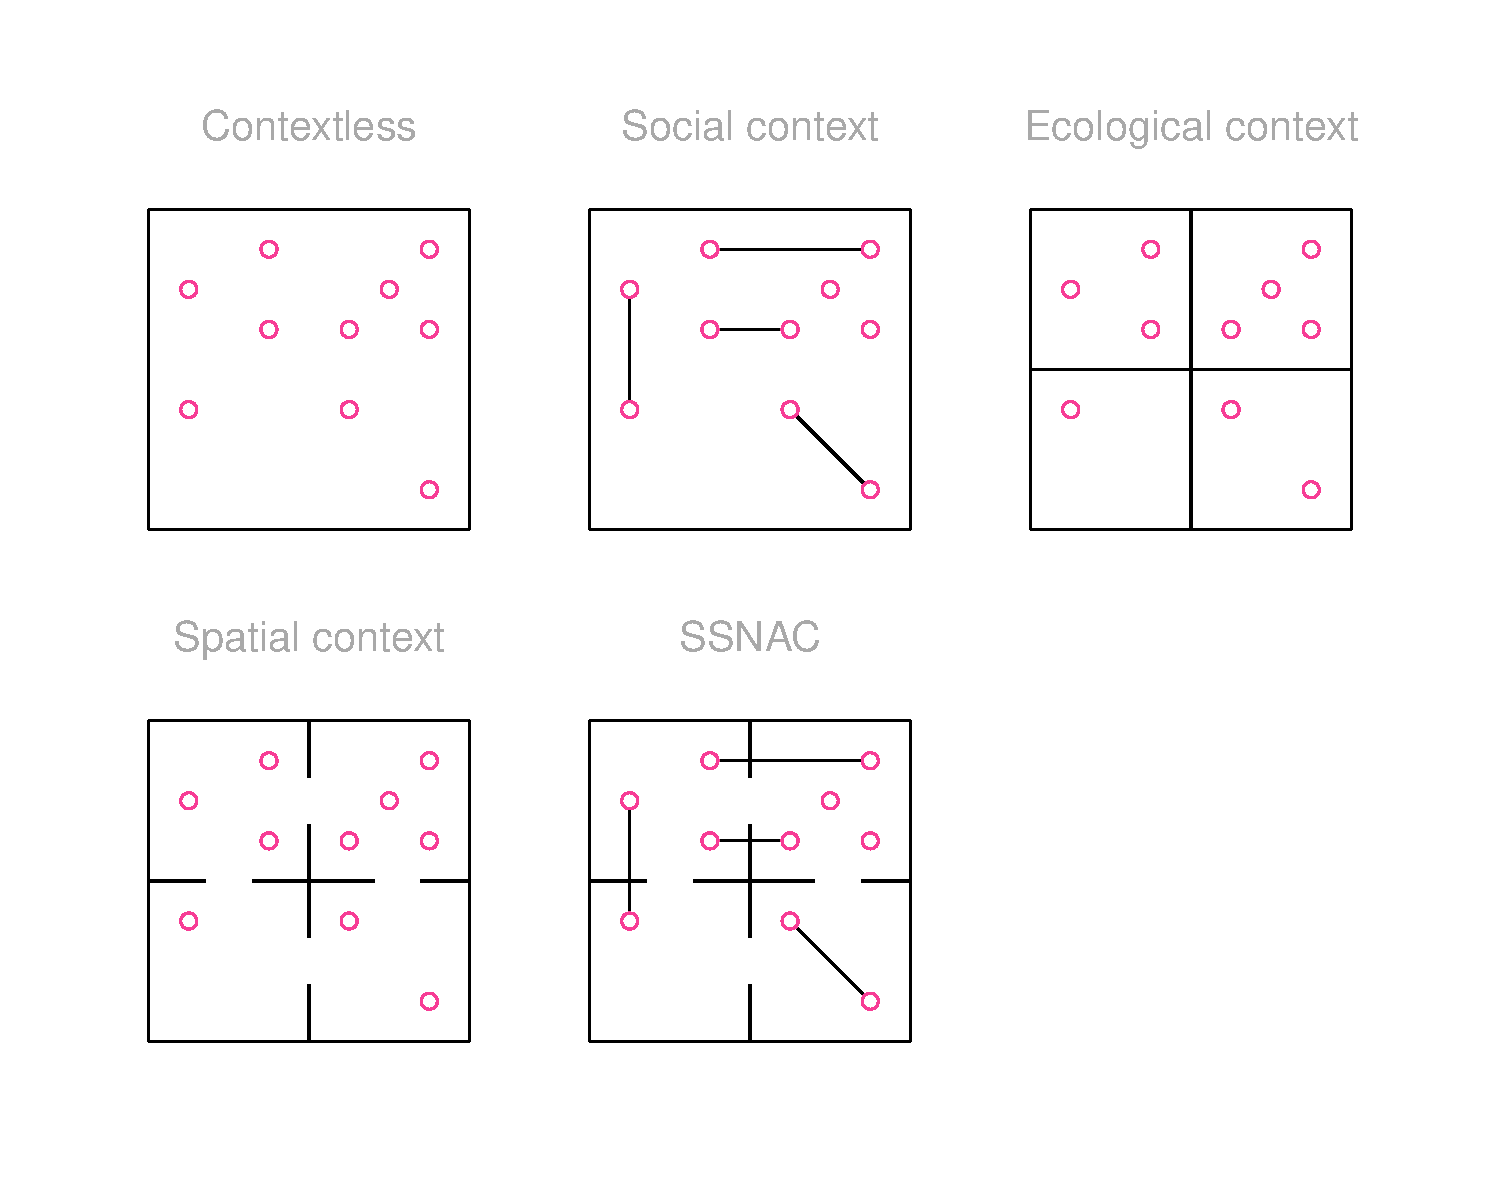
\includegraphics{A_ssnac1_social_spatial_context/A__ssnac1_social_spatial_context_files/figure-pdf/fig-context-1.pdf}

}

\caption{\label{fig-context}Approaches to incorporating context in
studies of individual health}

}

\end{minipage}%

\end{figure}

A social network analysis would gain a more granular understanding of
risk by assigning people who are connected to other people a higher risk
of acquiring the cold than those who have no relationships. In addition,
different connected components of the network could be assigned
differnet levels of risk.

An ecologic approach would be to divide up the area into households and
assign a different level of risk based on the household (third panel
from left). If we knew who has a cold, we could assign people in the
same household higher risk for acquiring the cold than others. This
anlysis, however, would ignore the fact that households are not equally
connected.

A spatial analysis would enhance this analysis by enriching household
data with a spatial weights matrix indicating which pairs of households
are neighrbors (second panel from right). Then the risk of aquiring a
cold in a given household would be a function of the risk of aquiring a
cold among individuals in neighboring households.

An SSNAC analysis (rightmost panel) would take advantage of both spatial
and social network data, assigning risk so that the risk of acquiring
the cold is a function of the household the individual belongs to, the
neighboring household, and the social network connections.

\hypertarget{ssnac-components}{%
\section{SSNAC components}\label{ssnac-components}}

The SSNAC framework is an approach to collecting, analyzing and
interpreting data which explicitly accounts for relationships among
people, the places they physical places they interact in or co-inhabit.

It is applicable in two situations: when investigators want to describe
the patterns in the relations among people, places, and across people
and places; or when investigators are interested in inferring causality
in the context of the system formed by people and places.

For the descriptive interest, it is necessary to have data on
individuals, the physical spatial units they co-inhabit, relationships
among individuals (network data), as well as the relationships among
spatial units (spatial weights matrix).

For the causal interest, it is necessary for the investigator should
have the data mentioned above, as well as a theory or set of theories
about the causal process under investigation. These theories must
explicitly state:

\begin{itemize}
\item
  the meaning of nodes (which entities they represent)
\item
  the meaning of ties (how they relate the entities they link)
\item
  an understanding of which ties are relevant to the causal question
  under investigation
\end{itemize}

\hypertarget{the-data-are-a-network}{%
\section{The data are a network}\label{the-data-are-a-network}}

The central data structure in a SSNAC is the person-place graph.
Figure~\ref{fig-ssnac} depicts the rightmost frame of
Figure~\ref{fig-context} by showing spatial units as nodes in a network,
connecting adjacent spatial units with a network edge, and connecting
individuals with the households they belong to. To show the flexibility
of this data object, we added an additional type of relationship an
individual can have with a household - that of an employee.

The majority of study data are stored as node or edge attributes. For
instance, person nodes might have attributes like age and race whereas
place nodes could have attributes like density or surface area. An edge
linking a person to a place might have an attribute conveying how the
person relates to the place. For instance in Figure~\ref{fig-ssnac},
some edges indicate residence, some indicate next

\begin{Shaded}
\begin{Highlighting}[]
\FunctionTok{plot\_ssnac\_example}\NormalTok{() }\SpecialCharTok{|\textgreater{}}
  \FunctionTok{style\_ssnac\_example}\NormalTok{() }\SpecialCharTok{+}
  \FunctionTok{theme\_mpxnyc\_blank}\NormalTok{()}
\end{Highlighting}
\end{Shaded}

\begin{figure}[H]

{\centering 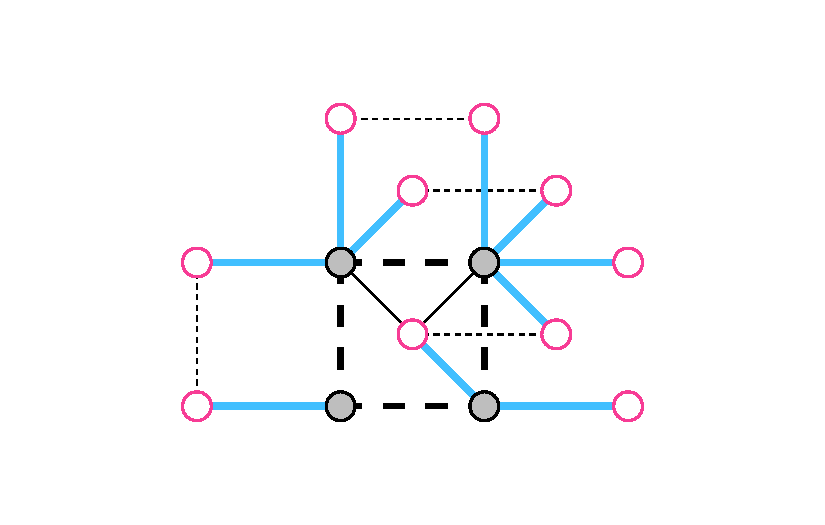
\includegraphics{A_ssnac1_social_spatial_context/A__ssnac1_social_spatial_context_files/figure-pdf/fig-ssnac-1.pdf}

}

\caption{\label{fig-ssnac}SSNAC Person-place graph}

\end{figure}

\hypertarget{the-network-is-a-causal-structure}{%
\section{The network is a causal
structure}\label{the-network-is-a-causal-structure}}

The Person-place graph is a starting point for constructing a causal
model, but it is not sufficient. Depending on the causal question, some
edges in this graph are relevant and some are not. For example, if we
were interested in a rumor network, we might decide to depict only
people and not places in the causal graph. We might also choose to
ignore the neighbor edges and focus only on the friend and employee
ones, if it is the case that rumours are transmitted within households
and across friendships but not to neighbors.

If we were interested in an infectious disease, and in the study
setting, there is a stay-at-home order so that friends do not meet, but
neighbors possibly meet, then we might keep the neighbor ties and drop
the friend and employee ties. In either case, it is necessary to make
changes to the Person-place network through network operations like
ignoring or adding ties, or even grouping nodes to form a different
graph altogether.

We explore this in the Analysis appendix.

\hypertarget{new-causal-structures-open-new-causal-enquiries}{%
\section{New causal structures open new causal
enquiries}\label{new-causal-structures-open-new-causal-enquiries}}

There are four types of causal queries that focus on node-level outcomes
in the SNACC framework.

\begin{itemize}
\item
  Person-To-Place: Evaluating the causal impact of a person-level
  intervention on place-level outcomes for some defined set of people
  and some defined set of places. e.g.~What is the impact of vaccinating
  college-aged adults in New York City on mpox incidence in Union Square
  (a favourite hangout spot for college students)
\item
  Person-to-Person: Evaluating the impact of a person-level intervention
  on person-level outcomes for some defined sets of people. e.g.~How
  does vaccinating all cisgender white men in New York City affect mpox
  incidence among Black and Latinx cisgender black men in New York City?
\item
  Place-to-Place: Evaluating the impact of a place-level intervention on
  place-level outcomes for some defined sets of places. e.g How does
  vaccinating Manhattan affect mpox incidence in Brooklyn?
\item
  Place-to-Person: Evaluating the impact of a place-level intervention
  on person-level outcomes for some defined set of people and some
  defined set of places. e.g.~How does vaccinating Harlem affect mpox
  incidence among cisgender black men in New York City
\end{itemize}

In addition there is an endless potential for constructing causal
queries that focus on characteristics that cannot be represented as node
characteristics for any single node, but rather are characteristics that
emerge as a result of the pattern of interactions among nodes. For
examples, see the section on social causal inference.

\hypertarget{sec-appendix-network-analysis}{%
\chapter{SSNAC II: Network
analysis}\label{sec-appendix-network-analysis}}

In this appendix we describe the main data objects of the MPX NYC study
- the Person-place graph, the Person graph and the Place graph. We
define measures used to analyze these graphs.

\hypertarget{data}{%
\section{Data}\label{data}}

\hypertarget{person-place-graph}{%
\subsection{Person-place graph}\label{person-place-graph}}

The MPX NYC spatial participant data network is a network object that
contains all collected data. In this network, nodes comprise of
community districts and survey participants. Edges can only exist
between a person and a communtiy district - they indicate that the
person either lives in or has a contact place in that community
district. In Figure~\ref{fig-example-participant-place}, participant
nodes are blue and community district nodes are pink.
Table~\ref{tbl-example-bipartite-nodes-edges} (a) shows the node and
Table~\ref{tbl-example-bipartite-nodes-edges} (b) the edges of the
network.

\begin{Shaded}
\begin{Highlighting}[]
\FunctionTok{make\_example\_network\_data}\NormalTok{(}\StringTok{"bipartite"}\NormalTok{) }\SpecialCharTok{|\textgreater{}}
  \FunctionTok{plot\_example\_network}\NormalTok{(targets}\SpecialCharTok{::}\FunctionTok{tar\_read}\NormalTok{(config\_list)) }\SpecialCharTok{+}
\NormalTok{  ggplot2}\SpecialCharTok{::}\FunctionTok{coord\_cartesian}\NormalTok{(}\AttributeTok{xlim=}\FunctionTok{c}\NormalTok{(}\SpecialCharTok{{-}}\DecValTok{2}\NormalTok{,}\DecValTok{3}\NormalTok{), }\AttributeTok{ylim=}\FunctionTok{c}\NormalTok{(}\SpecialCharTok{{-}}\FloatTok{1.2}\NormalTok{,}\FloatTok{1.2}\NormalTok{)) }\SpecialCharTok{+}
  \FunctionTok{theme\_mpxnyc\_blank}\NormalTok{() }\SpecialCharTok{+}
\NormalTok{  ggplot2}\SpecialCharTok{::}\FunctionTok{theme}\NormalTok{(}
    \AttributeTok{plot.margin =}\NormalTok{ ggplot2}\SpecialCharTok{::}\FunctionTok{margin}\NormalTok{(}\DecValTok{0}\NormalTok{,}\DecValTok{0}\NormalTok{,}\DecValTok{0}\NormalTok{,}\DecValTok{0}\NormalTok{)}
\NormalTok{  )}
\end{Highlighting}
\end{Shaded}

\begin{figure}[H]

{\centering 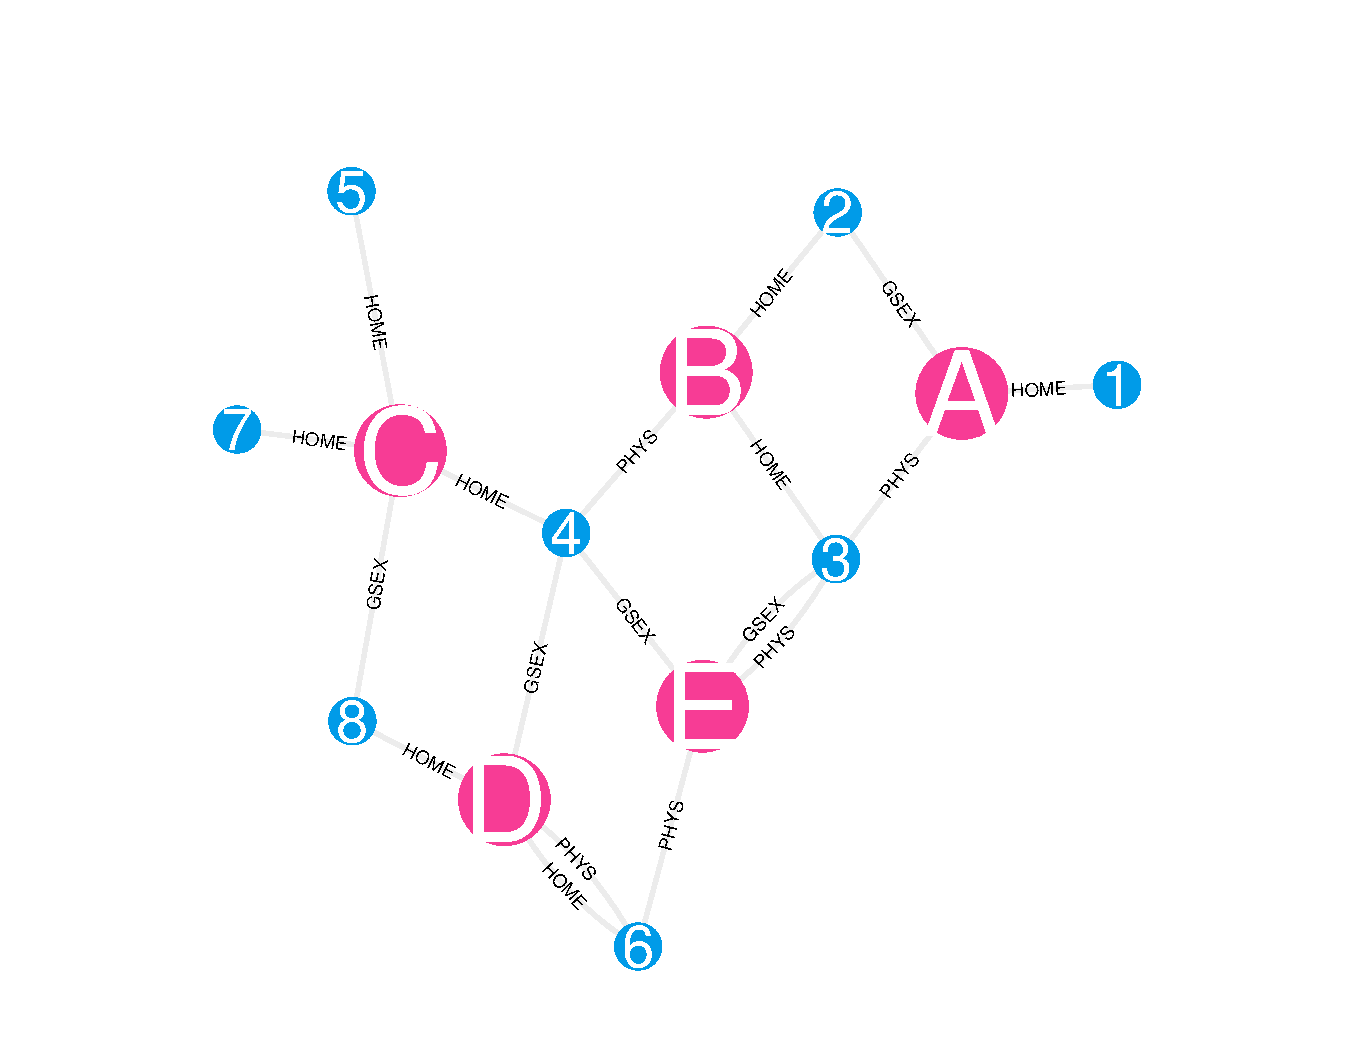
\includegraphics{B_ssnac2_network_analysis/B__ssnac2_network_analysis_files/figure-pdf/fig-example-participant-place-1.pdf}

}

\caption{\label{fig-example-participant-place}Sample person-place
network visualization}

\end{figure}

\begin{Shaded}
\begin{Highlighting}[]
\FunctionTok{make\_example\_network\_data}\NormalTok{() }\SpecialCharTok{|\textgreater{}}
  \FunctionTok{data.frame}\NormalTok{() }\SpecialCharTok{|\textgreater{}}
\NormalTok{  dplyr}\SpecialCharTok{::}\FunctionTok{transmute}\NormalTok{(}\AttributeTok{name =}\NormalTok{label, age, }\AttributeTok{type =} \FunctionTok{ifelse}\NormalTok{(type, }\StringTok{"Person"}\NormalTok{, }\StringTok{"Community District"}\NormalTok{)) }\SpecialCharTok{|\textgreater{}}
\NormalTok{  gt}\SpecialCharTok{::}\FunctionTok{gt}\NormalTok{()}
\FunctionTok{make\_example\_network\_data}\NormalTok{() }\SpecialCharTok{|\textgreater{}}
\NormalTok{  dplyr}\SpecialCharTok{::}\FunctionTok{mutate}\NormalTok{(}\AttributeTok{name =}\NormalTok{ label, type, age) }\SpecialCharTok{|\textgreater{}}
\NormalTok{  tidygraph}\SpecialCharTok{::}\FunctionTok{activate}\NormalTok{(edges) }\SpecialCharTok{|\textgreater{}}
\NormalTok{  dplyr}\SpecialCharTok{::}\FunctionTok{mutate}\NormalTok{(}\AttributeTok{from\_name =}\NormalTok{ tidygraph}\SpecialCharTok{::}\FunctionTok{.N}\NormalTok{()}\SpecialCharTok{$}\NormalTok{name[from], }\AttributeTok{to\_name =}\NormalTok{ tidygraph}\SpecialCharTok{::}\FunctionTok{.N}\NormalTok{()}\SpecialCharTok{$}\NormalTok{name[to]) }\SpecialCharTok{|\textgreater{}}
  \FunctionTok{data.frame}\NormalTok{() }\SpecialCharTok{|\textgreater{}}
\NormalTok{  dplyr}\SpecialCharTok{::}\FunctionTok{arrange}\NormalTok{(from, to) }\SpecialCharTok{|\textgreater{}}
\NormalTok{  dplyr}\SpecialCharTok{::}\FunctionTok{transmute}\NormalTok{(}\AttributeTok{From =}\NormalTok{ from\_name, }\AttributeTok{To =}\NormalTok{ to\_name, }\AttributeTok{Relation =}\NormalTok{ relation) }\SpecialCharTok{|\textgreater{}}
\NormalTok{  gt}\SpecialCharTok{::}\FunctionTok{gt}\NormalTok{()}
\end{Highlighting}
\end{Shaded}

\begin{table}

\caption{\label{tbl-example-bipartite-nodes-edges}Sample person-place
network data}\begin{minipage}[t]{0.50\linewidth}
\subcaption{\label{tbl-example-bipartite-nodes-edges-1}Nodes }

{\centering 

\begin{longtable}{lrl}
\tabularnewline

\toprule
Label & Age & Type \\ 
\midrule\addlinespace[2.5pt]
1 & 18-25 & Person \\ 
2 & 18-25 & Person \\ 
3 & 18-25 & Person \\ 
4 & 18-25 & Person \\ 
5 & 26-50 & Person \\ 
6 & 26-50 & Person \\ 
7 & 26-50 & Person \\ 
8 & 26-50 & Person \\ 
A & - & Community District \\ 
B & - & Community District \\ 
C & - & Community District \\ 
D & - & Community District \\ 
E & - & Community District \\ 
\bottomrule
\end{longtable}

}

\end{minipage}%
%
\begin{minipage}[t]{0.50\linewidth}
\subcaption{\label{tbl-example-bipartite-nodes-edges-2}Edges }

{\centering 

\begin{longtable}{rll}
\tabularnewline

\toprule
From & To & Relation \\ 
\midrule\addlinespace[2.5pt]
1 & A & HOME \\ 
2 & A & GSEX \\ 
2 & B & HOME \\ 
3 & A & PHYS \\ 
3 & B & HOME \\ 
3 & E & GSEX \\ 
3 & E & PHYS \\ 
4 & B & PHYS \\ 
4 & C & HOME \\ 
4 & D & GSEX \\ 
4 & E & GSEX \\ 
5 & C & HOME \\ 
6 & D & PHYS \\ 
6 & D & HOME \\ 
6 & E & PHYS \\ 
7 & C & HOME \\ 
8 & C & GSEX \\ 
8 & D & HOME \\ 
\bottomrule
\end{longtable}

}

\end{minipage}%

\end{table}

\hypertarget{person-graph}{%
\subsection{Person graph}\label{person-graph}}

The MPX NYC participant network has participants as nodes. A pair of
nodes is connected by a weighted edge if each of the individuals
represented by the nodes has at least one contact venue or residence in
the same, shared community district. The weight of the edge is given by
the count of community districts the pair of nodes have in common. By
definition, an edge of weight \(0\) is equivalent to the absence of an
edge. Table~\ref{tbl-example-participant-nodes} shows the nodes of the
participant network shown in Table~\ref{tbl-example-participant-nodes}
(a) and Table~\ref{tbl-example-participant-nodes} (b) show the edges.

\begin{Shaded}
\begin{Highlighting}[]
\FunctionTok{make\_example\_network\_data}\NormalTok{(}\StringTok{"people"}\NormalTok{) }\SpecialCharTok{|\textgreater{}}
  \FunctionTok{plot\_example\_network}\NormalTok{(targets}\SpecialCharTok{::}\FunctionTok{tar\_read}\NormalTok{(config\_list)) }\SpecialCharTok{+}
  \FunctionTok{theme\_mpxnyc\_blank}\NormalTok{()}
\end{Highlighting}
\end{Shaded}

\begin{figure}[H]

{\centering \includegraphics{B_ssnac2_network_analysis/B__ssnac2_network_analysis_files/figure-pdf/fig-example-participant-1.pdf}

}

\caption{\label{fig-example-participant}Sample person-person network
visualizatoin}

\end{figure}

\begin{Shaded}
\begin{Highlighting}[]
\FunctionTok{make\_example\_network\_data}\NormalTok{(}\StringTok{"people"}\NormalTok{) }\SpecialCharTok{|\textgreater{}}
  \FunctionTok{data.frame}\NormalTok{() }\SpecialCharTok{|\textgreater{}}
\NormalTok{  dplyr}\SpecialCharTok{::}\FunctionTok{transmute}\NormalTok{(}\AttributeTok{Name =}\NormalTok{ label, }\AttributeTok{Type =} \FunctionTok{ifelse}\NormalTok{(type, }\StringTok{"Person"}\NormalTok{, }\StringTok{"Community District"}\NormalTok{)) }\SpecialCharTok{|\textgreater{}}
\NormalTok{  gt}\SpecialCharTok{::}\FunctionTok{gt}\NormalTok{()}
\FunctionTok{make\_example\_network\_data}\NormalTok{(}\StringTok{"people"}\NormalTok{) }\SpecialCharTok{|\textgreater{}}
\NormalTok{  dplyr}\SpecialCharTok{::}\FunctionTok{mutate}\NormalTok{(}\AttributeTok{name =}\NormalTok{ label, type, age) }\SpecialCharTok{|\textgreater{}}
\NormalTok{  tidygraph}\SpecialCharTok{::}\FunctionTok{activate}\NormalTok{(edges) }\SpecialCharTok{|\textgreater{}}
\NormalTok{  dplyr}\SpecialCharTok{::}\FunctionTok{mutate}\NormalTok{(}\AttributeTok{from\_name =}\NormalTok{ tidygraph}\SpecialCharTok{::}\FunctionTok{.N}\NormalTok{()}\SpecialCharTok{$}\NormalTok{name[from], }\AttributeTok{to\_name =}\NormalTok{ tidygraph}\SpecialCharTok{::}\FunctionTok{.N}\NormalTok{()}\SpecialCharTok{$}\NormalTok{name[to]) }\SpecialCharTok{|\textgreater{}}
  \FunctionTok{data.frame}\NormalTok{() }\SpecialCharTok{|\textgreater{}}
\NormalTok{  dplyr}\SpecialCharTok{::}\FunctionTok{arrange}\NormalTok{(from, to) }\SpecialCharTok{|\textgreater{}}
\NormalTok{  dplyr}\SpecialCharTok{::}\FunctionTok{transmute}\NormalTok{(}\AttributeTok{From =}\NormalTok{ from\_name, }\AttributeTok{To =}\NormalTok{ to\_name, }\AttributeTok{Weight =}\NormalTok{ weight) }\SpecialCharTok{|\textgreater{}}
\NormalTok{  gt}\SpecialCharTok{::}\FunctionTok{gt}\NormalTok{()}
\end{Highlighting}
\end{Shaded}

\begin{table}

\caption{\label{tbl-example-participant-nodes}Sample person-person
network data}\begin{minipage}[t]{0.50\linewidth}
\subcaption{\label{tbl-example-participant-nodes-1}Nodes }

{\centering 

\begin{longtable}{rl}
\tabularnewline

\toprule
Name & Type \\ 
\midrule\addlinespace[2.5pt]
1 & Person \\ 
2 & Person \\ 
3 & Person \\ 
4 & Person \\ 
5 & Person \\ 
6 & Person \\ 
7 & Person \\ 
8 & Person \\ 
\bottomrule
\end{longtable}

}

\end{minipage}%
%
\begin{minipage}[t]{0.50\linewidth}
\subcaption{\label{tbl-example-participant-nodes-2}Edges }

{\centering 

\begin{longtable}{rrr}
\tabularnewline

\toprule
From & To & Weight \\ 
\midrule\addlinespace[2.5pt]
1 & 2 & 1 \\ 
1 & 3 & 1 \\ 
2 & 3 & 2 \\ 
2 & 4 & 1 \\ 
3 & 4 & 3 \\ 
3 & 6 & 2 \\ 
4 & 5 & 1 \\ 
4 & 6 & 3 \\ 
4 & 7 & 1 \\ 
4 & 8 & 2 \\ 
5 & 7 & 1 \\ 
5 & 8 & 1 \\ 
6 & 8 & 2 \\ 
7 & 8 & 1 \\ 
\bottomrule
\end{longtable}

}

\end{minipage}%

\end{table}

\hypertarget{place-graph}{%
\subsection{Place graph}\label{place-graph}}

The MPX NYC community district network has community districts as nodes.
A pair of community districts is connected by a weighted edge when at
least one participant has a contact venue or residence in both community
districts. The weight is the count of participants which are shared by
the two community districts. Figure~\ref{fig-example-community} shows
the community district network derived from the MPX NYC spatial
participant data network shown in
Figure~\ref{fig-example-participant-place}.
Table~\ref{tbl-example-place-nodes} (a) shows list the nodes of the
former network, and Table~\ref{tbl-example-place-nodes} (b) shows the
edges.

\begin{Shaded}
\begin{Highlighting}[]
\FunctionTok{make\_example\_network\_data}\NormalTok{(}\StringTok{"places"}\NormalTok{) }\SpecialCharTok{|\textgreater{}}
  \FunctionTok{plot\_example\_network}\NormalTok{(targets}\SpecialCharTok{::}\FunctionTok{tar\_read}\NormalTok{(config\_list))  }\SpecialCharTok{+}
  \FunctionTok{theme\_mpxnyc\_blank}\NormalTok{()}
\end{Highlighting}
\end{Shaded}

\begin{figure}[H]

{\centering 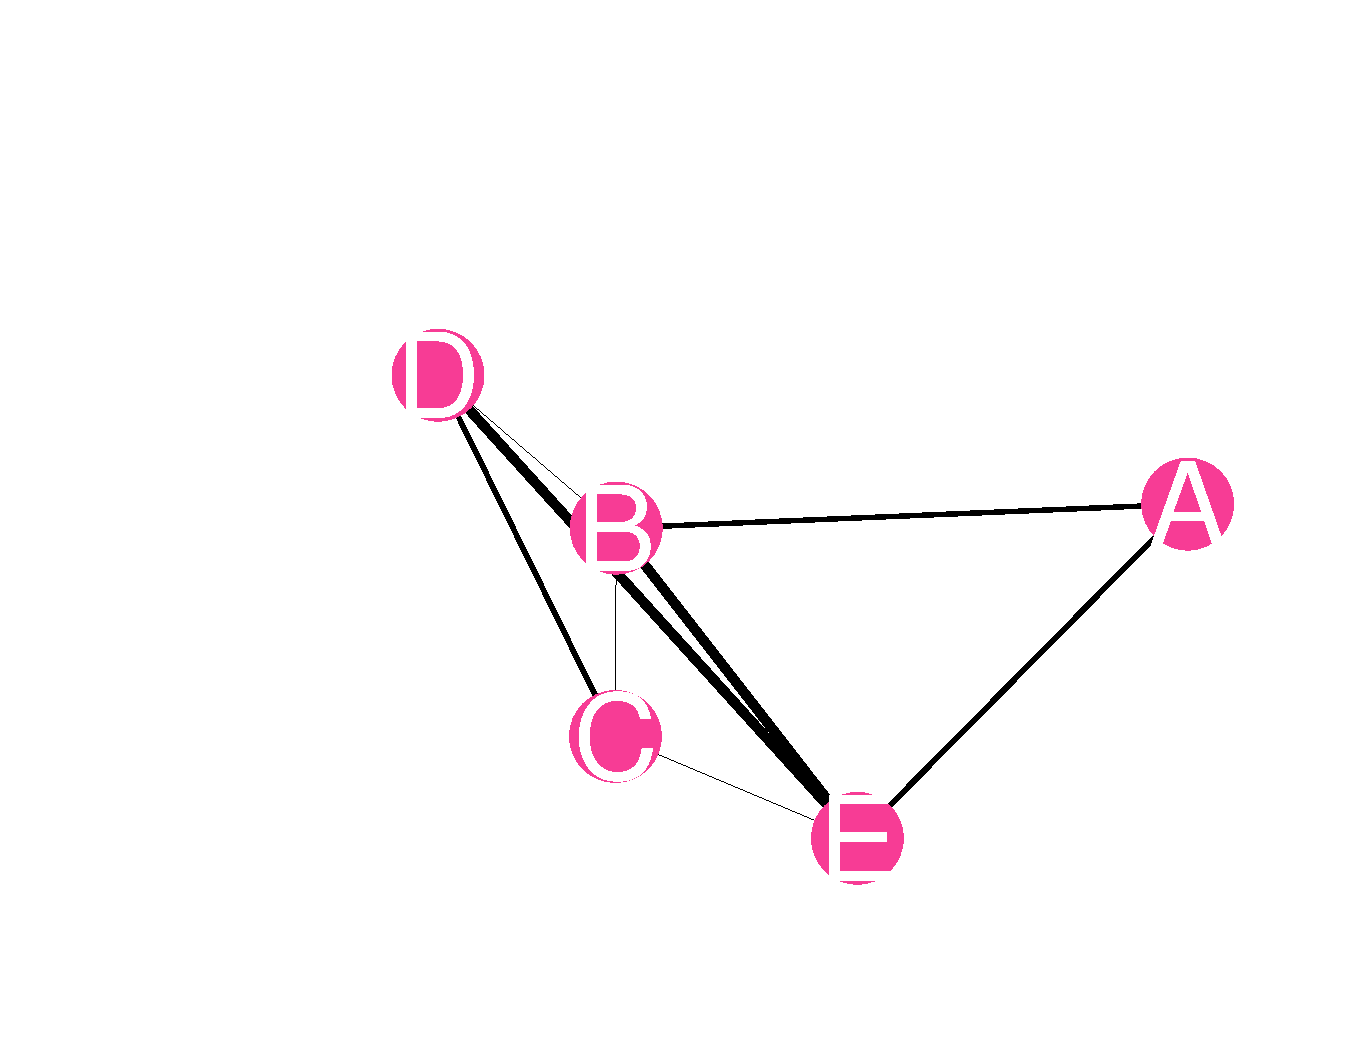
\includegraphics{B_ssnac2_network_analysis/B__ssnac2_network_analysis_files/figure-pdf/fig-example-community-1.pdf}

}

\caption{\label{fig-example-community}Sample place network
visualization}

\end{figure}

\begin{Shaded}
\begin{Highlighting}[]
\FunctionTok{make\_example\_network\_data}\NormalTok{(}\StringTok{"places"}\NormalTok{) }\SpecialCharTok{|\textgreater{}}
  \FunctionTok{data.frame}\NormalTok{() }\SpecialCharTok{|\textgreater{}}
\NormalTok{  dplyr}\SpecialCharTok{::}\FunctionTok{transmute}\NormalTok{(}\AttributeTok{Name =}\NormalTok{ label, }\AttributeTok{Type =} \FunctionTok{ifelse}\NormalTok{(type, }\StringTok{"Person"}\NormalTok{, }\StringTok{"Community District"}\NormalTok{)) }\SpecialCharTok{|\textgreater{}}
\NormalTok{  gt}\SpecialCharTok{::}\FunctionTok{gt}\NormalTok{()}
\FunctionTok{make\_example\_network\_data}\NormalTok{(}\StringTok{"places"}\NormalTok{) }\SpecialCharTok{|\textgreater{}}
\NormalTok{  dplyr}\SpecialCharTok{::}\FunctionTok{mutate}\NormalTok{(}\AttributeTok{name =}\NormalTok{ label, type, age) }\SpecialCharTok{|\textgreater{}}
\NormalTok{  tidygraph}\SpecialCharTok{::}\FunctionTok{activate}\NormalTok{(edges) }\SpecialCharTok{|\textgreater{}}
\NormalTok{  dplyr}\SpecialCharTok{::}\FunctionTok{mutate}\NormalTok{(}\AttributeTok{from\_name =}\NormalTok{ tidygraph}\SpecialCharTok{::}\FunctionTok{.N}\NormalTok{()}\SpecialCharTok{$}\NormalTok{name[from], }\AttributeTok{to\_name =}\NormalTok{ tidygraph}\SpecialCharTok{::}\FunctionTok{.N}\NormalTok{()}\SpecialCharTok{$}\NormalTok{name[to]) }\SpecialCharTok{|\textgreater{}}
  \FunctionTok{data.frame}\NormalTok{() }\SpecialCharTok{|\textgreater{}}
\NormalTok{  dplyr}\SpecialCharTok{::}\FunctionTok{arrange}\NormalTok{(from, to) }\SpecialCharTok{|\textgreater{}}
\NormalTok{  dplyr}\SpecialCharTok{::}\FunctionTok{transmute}\NormalTok{(}\AttributeTok{From =}\NormalTok{ from\_name, }\AttributeTok{To =}\NormalTok{ to\_name, }\AttributeTok{Weight =}\NormalTok{ weight) }\SpecialCharTok{|\textgreater{}}
\NormalTok{  gt}\SpecialCharTok{::}\FunctionTok{gt}\NormalTok{()}
\end{Highlighting}
\end{Shaded}

\begin{table}

\caption{\label{tbl-example-place-nodes}Sample place network
data}\begin{minipage}[t]{0.50\linewidth}
\subcaption{\label{tbl-example-place-nodes-1}Nodes }

{\centering 

\begin{longtable}{ll}
\tabularnewline

\toprule
Name & Type \\ 
\midrule\addlinespace[2.5pt]
A & Community District \\ 
B & Community District \\ 
C & Community District \\ 
D & Community District \\ 
E & Community District \\ 
\bottomrule
\end{longtable}

}

\end{minipage}%
%
\begin{minipage}[t]{0.50\linewidth}
\subcaption{\label{tbl-example-place-nodes-2}Edges }

{\centering 

\begin{longtable}{llr}
\tabularnewline

\toprule
From & To & Weight \\ 
\midrule\addlinespace[2.5pt]
A & B & 2 \\ 
A & E & 2 \\ 
B & C & 1 \\ 
B & D & 1 \\ 
B & E & 3 \\ 
C & D & 2 \\ 
C & E & 1 \\ 
D & E & 3 \\ 
\bottomrule
\end{longtable}

}

\end{minipage}%

\end{table}

\hypertarget{measures}{%
\section{Measures}\label{measures}}

In this section, we describe network measures that are both useful
statistics to interpret in describing MPX NYC data and useful
intermediate steps in other measures we constructed.

We defined four measures related to node degree which offer a useful
interpretation of MPX NYC data: participant social reach (\(R_i\)),
participant spatial reach (\(S_i\)), community district social reach
(\(r_j\)), and community district spatial reach (\(s_j\)). For each of
these, we developed a measure for which we count only the connections to
nodes which are included in some defined subset \(A \subset N\) of
nodes. We thus define conditional participant social reach (\(R_i|A\)),
conditional participant spatial reach (\(S_i|A\)), conditional community
district social reach (\(r_j|A\)), and conditional community district
spatial reach (\(s_j|A\)).

We further defined two measures which summarize the pattern of
connection across the people and places in the MPX NYC dataset. The
first, the spatial mixing coefficient, can be used to analyze the
pattern of connection across different demographic groups. The second,
proportion in largest connected component, can be used to analyze the
overall connectedness of the MPX NYC Person-Place graph and related
graphs.

\hypertarget{notation}{%
\subsection{Notation}\label{notation}}

Define \(\psi(i,j)\) as the adjacency function for the person-place
graph. For person \(i\) and community \(j\):

\[
\psi(i,j) = \begin{cases} 1 &i\sim j \\ 0 &\text{otherwise} \end{cases}
\]

Define \(\psi_P(i,k)\) as the adjacency functon for the person graph.
For persons \(i\) and \(k\):

\[
\psi_P(i,k) = \sum_{j \in N_C}{\psi(i,j) \psi(k,j)}
\]

Define \(\psi_C(j,l)\) as the adjacency functon for the place graph. For
places \(j\) and \(l\):

\[
\psi_C(j,l) = \sum_{i \in N_P}{\psi(i,j) \psi(i,l)}
\]

\hypertarget{node-characteristics-1}{%
\subsection{Node characteristics}\label{node-characteristics-1}}

\hypertarget{participant-social-reach}{%
\subsubsection{Participant social
reach}\label{participant-social-reach}}

Participant social reach is defined as weighted node degree in the MPX
NYC participant network. For participant \(i \in N_p\)

\[
R_i = \sum_{j \in N_p}{\psi_p (i,j)}
\]

\[
R_i | A= \sum_{j \in N_p}{\psi_p (i,j)I_{x \in A}(x = j) }
\]

where the indicator function \(I_{x \in A}(x)\) equals \(1\) when
\(x\in A\) and \(0\) otherwise.

\hypertarget{participant-spatial-reach}{%
\subsubsection{Participant spatial
reach}\label{participant-spatial-reach}}

Participant spatial reach is defined as the number of connections the
focal participant has with community districts. It is defined as the
weighted node degree in the MPX NYC spatial participant network. For
\(i \in N_p\)

\[
S_i = \sum_{j \in N_c}{\psi (i,j)}
\]

\[
S_i|A = \sum_{j \in N_c}{\psi (i,j)I_{x \in A}(x = j)}
\]

\hypertarget{community-district-social-reach}{%
\paragraph{Community district social
reach}\label{community-district-social-reach}}

Community district social reach is defined as the number of connections
the focal community district has with participants. It is defined as the
weighted node degree in the MPX NYC spatial participant network. For
\(j \in N_c\):

\[
r_j = \sum_{i \in N_p}{\psi (i, j)}
\]

\[
r_j|A = \sum_{i \in N_p}{\psi (i, j)I_{x \in A}(x = i)}
\]

\hypertarget{community-district-spatial-reach}{%
\paragraph{Community district spatial
reach}\label{community-district-spatial-reach}}

Community district spatial reach is defined as the weighted node degree
in the MPX NYC community district network. For \(j \in N_c\)

\[
s_j = \sum_{i \in N_c}{\psi_c (i,j)}
\]

\[
s_j|A = \sum_{i \in N_c}{\psi_c (i,j)I_{x \in A}(x = i)}
\]

\hypertarget{network-characteristics-1}{%
\subsection{Network characteristics}\label{network-characteristics-1}}

\hypertarget{movement-matrix}{%
\subsubsection{Movement matrix}\label{movement-matrix}}

Define \(d^H(i)\) as the home district of person \(i\). The movement
coefficient \(m(k,l)\) is defined as the count of connections by
individuals \(i\) who live in home community district \(k\) with
community districts \(l\).

\[
m(k,l) = \sum_{i \in \mathscr{N}_P} \sum_{j \in \mathscr{N}_C} \psi_C (d^H(i),j)I_{d^H(x)=k}(i)I_{x=l}(j)
\]

The movement matrix is a square matrix whose \(ij^{th}\) entry is
\(m(i,j)\).

\hypertarget{spatial-concentration-chart}{%
\subsubsection{Spatial concentration
chart}\label{spatial-concentration-chart}}

The spatial concentration proportion \(c(k)\) quantifies the degree to
which a community district is over-represented among destination
community districts compared to home districts in the movement matrix.
It is the difference of the margins of the movement matrix. For
community district k

\[
c(k) = \frac{\sum_l{m(l,k) - m(k,l)}}{\sum_{i,j}{m(i,j)}}
\]

The spatial concentration chart plots teh spatial concentration
proprotion for each community district.

\hypertarget{spatial-mixing-matrix}{%
\subsubsection{Spatial mixing matrix}\label{spatial-mixing-matrix}}

The MPX NYC participant network can also be used to analyze the pattern
of connection across different demographic groups. We did this using the
spatial mixing coefficient, which we motivate and define below.

Say there are three types of retired university professors in Boston -
A) those who choose to live and socialize in neighborhoods with
universities (where they can meet old colleagues and students); B) those
who choose to live and socialize away from former colleagues and
students; and C) those who choose neighborhoods without regard for
university life. And say the proportion of people who are under 25 years
of age in Boston is \(20\%\) and that the majority of this group are
college students. People who are under 25 years of age would be
over-represented in neighborhoods with college campuses and residences,
and under-represented in those without.

To understand what kind of retired professor a particular person is, you
could ask her of all the peopple she encountered in the past 12 months,
what proportion were under \(25\). If she is of type C, we would expect
her answer to be about \(20\%\). If she avoids universities (i.e.~is of
type B), the proportion would be lower than \(20\%\) and if she seeks
them out (i.e.~type A), her answer would be greater than \(20\%\).

In the motivating example, we were soliciting the retired professor's
preference for the subgroup: under 25. We were then mentally comparing
it with the prevalence of that subgroup (\(20\%\)). The spatial mixing
coefficient makes this comparison by dividing preference by prevalence
and subtracting 1. It is zero when contact venues and residences for a
given subgroup are distributed in space independently of another;
positive if members of the former subgroup tend to share community
districts with those of the latter; and negative if they tend to not
share community districts.

The spatial mixing coefficient is related to notions in social network
analysis and compartmental infectious disease modelling. The coefficient
of a given sub-group for that same subgroup indicates homophily when it
is positive, random mixing when it is zero, and heterophily when it is
negative. It goes further by showing, in the case of heterophily, which
subgroups members of the focal subgroup tend to be connected with. This
is useful in early outbreak investigations as it allows the analyst to
understand the potential path of a new pathogen across the population of
interest. e.g.~where there is strong homophily in the a network like the
MPX NYC participant network, a new pathogen will tend to stay within the
subgroup it first affected. If there is strong heterophily, on the other
hand, the pathogen will tend to disseminate across groups favored by the
first subgroup it affected.

We define preference of group A for group B (\(\Phi(A,B)\)) as the
average proportion of alters from group B among egos from group A.

\[
\Phi(A,B) = \frac{1}{|A|}\sum_{i \in A}{\frac{ R_i | B}{R_i}}
\]

To understand whether preference of a specific group by another group is
higher or lower than we would expect if ego's chose alters randomly, we
compare preference for B to the prevalence of group B:

\[
 \frac{|B|}{|N_p|}
\]

The spatial mixing coefficient is the ratio of preference to prevalence
minus one:

\[
\phi(A,B) = \frac{|N_p|}{|B|} \Phi(A,B) - 1
\]

\hypertarget{proportion-in-largest-connected-component}{%
\subsubsection{Proportion in largest connected
component}\label{proportion-in-largest-connected-component}}

In a given network, a connected component is a subset of nodes such that
each node in the subset is reachable from any other node in the subset,
and such that there are no nodes outside the subset which are reachable
from a node inside it. By reachable, we mean possible to reach by
tracing a path from one node to another over existing network ties.

In the MPX NYC participant network, it is possible to uniquely partition
the node set \(N_p\) into connected components. This follows from the
facts that connected components form non-overlapping subsets of \(N_p\)
and that it is possible to write \(N_p\) as a union of subsets \(C_k\)
which are each connected components.

\[
N = \bigcup_{k = 1}^{K}{C_k}
\]

We define the proportion in the largest connected component as:

\[
\theta_p = \frac{\max_k{|C_k|}}{|N_p|}
\]

\hypertarget{ssnac-iii-causal-interpretation}{%
\chapter{SSNAC III: Causal
interpretation}\label{ssnac-iii-causal-interpretation}}

\leavevmode\vadjust pre{\hypertarget{authors}{}}%
Keletso Makofane, PhD

RESPND-MI Collaboration

In this appendix we contextualize the main analysis in the MPX NYC
project using a framework we name Social and Spatial Network Analysis
with Causal interpretation (SNACC). The SSNAC framework can be used to
guide the collection, management, analysis, and causal interpretation of
network data. It offers guidance on conceptualizing and organizing
spatial and social data as networks
(Appendix~\ref{sec-appendix-social-spatial}) and provides tools for
descriptive and causal analysis
(Appendix~\ref{sec-appendix-network-analysis}).

In this section we elaborate the ``causal interpretation'' aspect of
SSNAC. We define SSNAC as a set of straight-forward extensions of the
currently dominant framework for conducting causal inference with
observational data in epidemiology. We begin by giving an overview of
the dominant approach, which we will call ``classic causal inference''.
We extend this system to situations where data are characterized by
interdependence of observational units rather than independence, naming
this system ``network causal inference''. Finally, we accommodate social
and spatial data simultaneously in the SSNAC framework. In each case, we
describe the assumptions and implications of each system, illustrating
with worked examples.

Classic causal inference, as articulated by Robins (1986), Hernán
(2018), and others helps us to sharpen epidemiologic reasoning by
providing a template for conducting thought experiments about population
health. Typically in these thought experiments, the researcher reasons
about the likely effect of some hypothetical individual-level
intervention on some hypothetical outcome in some hypothetical
population. Through transparent statistical assumptions, the quantities
of interest in the thought experiment are calculated as a function of
observed or observable data.

For instance, consider a hypothetical intervention where every person in
the United States receives free, unlimited access to healthcare. Under
classic causal inference, we can ask whether the prevalence of diabetes
would change if we implemented the intervention. We can even ask about
the extent of change and estimate that using data that have already been
observed. The classic causal inference framework allows this by:

\begin{itemize}
\item
  making causal assumptions about the relationship between healthcare
  access and diabetes prevalence
\item
  mathematically stating the hypothetical quantities we are interested
  in
\item
  estimating those quantities using data we have or can collect about
  access to healthcare, diabetes prevalence, and any factor that
  determine both access and prevalence
\end{itemize}

A strong assumption made almost universally by practitioners of classic
causal inference is that of independence between observational units or
groups of observational units. In our opening example, this assumption
holds that one person's access to healthcare does not affect any other
person's diabetes status. It would imply that the diabetes status for a
married man who does not know how to cook, for instance, would not at
all be affected by improvements in health literacy experienced by his
wife who cooks for the household. The assumption of independence runs
counter to our intuitions about social life. Humans are networked - our
lives are defined by our relationships with others.

The choice of adopting the independence assumption or not has profound
implications for how we think about our inferential goals. In the
frequentist tradition of statistics, the engine of uncertainty is
repetition. We imagine that an experiment could be repeated over and
over again and we summarize its behavior across those imagined
repetitions. We do not often consider what exactly we mean by experiment
and by repetition, though we make this distinction each time we decide
how to analyse repeated-measures data.

An example to clarify: Consider a situation with two people, Jose and
Thabo, who each toss the same coin once at time 1 and again at time 2.
There are several ways of parsing this situation into ``experiment'' and
``repetition''. We could say that we are conducting:

\begin{itemize}
\item
  one experiment called ``coin toss'' and repeating it four times
\item
  two experiments called ``Thabo tosses a coin'' and ``Tumi tosses a
  coin'' and repeating each experiment twice
\item
  two experiments called ``coin toss at time 1'' and ``coin toss at time
  2'' and repeating each experiment twice
\item
  four experiments called ``Thabo tosses a coin at time 1'', ``Thabo
  tosses a coin at time 2'', ``Tumi tosses a coin at time 1'', and
  ``Tumi tosses a coin at time 2 and not repeating any of them.
\end{itemize}

The choice between these interpretations turns on the experimenters
prior beliefs about coin tossing: Does the likelihood of a head or tail
change over time? Does it change based on the person tossing the coin?
This kind of consideration is at the core statistical modelling,
particularly when analyzing longitudinal data.

One consideration researchers do not often make is whether one person's
coin toss is correlated with the other's. Consider the experiment
``Thabo tosses a coin, then Tumi tosses a coin, then Thabo tossess a
con, then Tumi tosses a coin''. Whereas in the above listing, by virture
of calling them separate experiments, we implicitly assumed that each
coin toss was self-contained, in this latest iteration, we accommodate
the possibility that the result of Thabo's coin toss affects the result
of Tumi's.

We can quantitatively assess this possibility by repeating this sequence
of coin tosses over and over, using that data to calculate a correlation
coefficient between the outcomes of Thabo and Tumi's coin tosses.
Without stating the experiment as this sequence, we have no framework
with which to ask whether Thabo and Tumi's coin tosses are causally
related.

In epidemiologic practice, the modelling decision to categorize people
or groups of people as independent of each other is so well-entrenched
that it is often presented as a necessary condition for doing any valid
causal quantitative research. Unlike it is with coins, however, with
humans, there is a mountain of evidence and experience proving
interdependence as the rule rather than the exception.

Our goal in this appendix and project is to offer alternative ideas and
tools for causal inference that allow researchers to learn from
interdependence rather than avoid it in pursuit of clear causal
reasoning. We can have both clear reasoning and an understanding
enriched by the analysis of dependent happenings.

In crude terms, our approach involves moving from a framework where, as
a rule, we consider Thabo and Jose's coin tosses one experiment, rather
than break it up into four. i.e.~Rather than define a scalar random
variable to represent a measure made on \(n\) individuals, we will
define a vector-valued random variable of length \(n\) and assume that
some of the entries in that random variable are correlated as a result
of being part of the same causal structure. But why would a researcher
want to do that when our tools for statistical modelling require as many
repetitions as possible for valid inferences? How can we quantify
uncertainty when we always have a sample size of 1?

Briefly, we can avail ourselves of asymptotic theory by making the
assumption of no-spillover between observations, which is a weaker
version of the independence between observational units assumption. No
spillover means that one person's outcome can not directly affect
another's. We further assume that the causal relationships between and
within individuals are homogeneous in some way, allowing our estimates
to benefit from having more observational units, even if they
collectively comprise one realization of the statistical model.

Under some mild assumptions, asymptotic theory can be used to improve
estimates in a growing vector of inter-related observations, whereas it
is usually applied to a growing collection of vectors of equal length.
In the network causal inference and SSNAC section, we construct model
restrictions which help to limit how quickly the number of potential
outcomes to estimate grows in relation to the number of observational
units.

In the sections that follow, we describe classic causal inference,
network causal inference, and the SSNAC framework, each time discussing
the assumptions, causal model, causal estimands, and illustrating a
causal identification strategy for the framework. Finally, we describe
the MPX NYC outbreak response analysis presented in the main report
using the SSNAC framework.

\hypertarget{sec-classic-causal-inference}{%
\section{Classic causal inference}\label{sec-classic-causal-inference}}

\hypertarget{example-1-dress-and-jobs}{%
\subsection*{Example 1: Dress and Jobs}\label{example-1-dress-and-jobs}}
\addcontentsline{toc}{subsection}{Example 1: Dress and Jobs}

We are interested in settling an argument among friends about the
relationship between dressing in formal wear and job offers. One friend
thinks that dressing formally brings more job offers; everyone she knows
who dresses formally has many more job offers than those who dress
casually.

The other friend thinks that what really brings job offers is currently
having a job. In their reasoning, having a job causes people to dress
formally and also causes people to receive job offers, but dressing
formally does not in itself improve a person's likelihood of receiving
job offers. We conduct a study to investigate.

We recruit three people, \emph{Person 1}, \emph{Person 2}, and
\emph{Person 3}. \emph{Person 1} and \emph{Person 2} are married to each
other. \emph{Person 1} and \emph{Person 3} are newly acquainted
colleagues. Say \emph{Person 1} has job status \(L_1\), \emph{Person 2}
has job status \(L_2\) and \emph{Person 3} has job status \(L_3\). Each
of these variables can only take on two values: ``employed
vs.~unemployed''. Similarly we define \(A_i\) as \emph{Person \(i\)'s}
dress (formal vs.~informal), and \(Y_i\) as their job offers (many
vs.~few). The job status measurement (\(L_i\)) precedes dress (\(A_i\))
in time, and dress precedes job offers (\(Y_i\)).

Before we continue with the example, we give a brief overview of the
non-parametric structural equation model with independent errors
(NPSEM-IE). This statistical model underpins the practice of using
counterfactual variables and directed acyclic graphs (DAGs) to reason
about causality.

\hypertarget{npsem-ie}{%
\subsection*{NPSEM-IE}\label{npsem-ie}}
\addcontentsline{toc}{subsection}{NPSEM-IE}

An NPSEM-IE is a system of equations which relates all the entries in a
given vector-valued random variable with each other. It does so without
specifying parametric functions for each equation in the system. An
example of such a model is shown by
Equation~\ref{eq-fullly-connected-dag}. In this set of equations, values
that are produced by equations higher up in the list are the inputs of
equations lower down on the list. The functions \(f_*\) are
deterministic, though their form is not necessarily known. The arguments
\(U_*\) represent error terms - random variables which are independent
of each other within and across observational units.

Whereas parametric models, for instance, a linear regression model with
normally distributed errors, are characterized by their probability
density functions, non-parametric models of this type are usually
characterized by their conditional independencies. An example of a
conditional independence statement would be:

\emph{for a realization \([X_1, X_2, X_3, X_4, X_5]\) of statistical
model \(F\)},

\[
X_1 \perp X_3 | X_2, X_4
\]

which reads: ``\emph{random variables \(X_1\) and \(X_3\) are
independent conditional on random variables \(X_2\) and \(X_4\)}''.

Non-parametric structural equation models are usually represented using
the Directed Acyclic Graph (DAG), which is a schematic representation of
the structural equations in the model. The DAG shown in
Figure~\ref{fig-fullly-connected-dag}, for instance, represents the
model defined by Equation~\ref{eq-fullly-connected-dag}. The arrow
pointing from \(L_1\) to \(L_3\), for instance, indicates that \(L_1\)
is an input in the structural equation for \(L_3\).

DAGs graphically encode the conditional independencies that characterize
non-parametric structural equation models. Using a DAG and a set of
rules called d-separation, it is possible to read from the DAG the set
of conditional independencies that imply all the conditional
independencies that characterize the model.

Conditional indpendencies are indicated by missing edges in the DAG. If
we made no assumptions at all about the causal process in Example 1
except the time-ordering of measurements, we could represent our data
using Equation~\ref{eq-fullly-connected-dag}. Since there are no missing
edges between nodes in the Figure~\ref{fig-fullly-connected-dag}, the
structural equation model represents any possible joint distribution
between the variables in the DAG - there are no conditional
independencies.

\begin{Shaded}
\begin{Highlighting}[]
\FunctionTok{make\_dag}\NormalTok{(}\StringTok{"fully\_connected"}\NormalTok{)         }\SpecialCharTok{|\textgreater{}} 
  \FunctionTok{plot\_swig}\NormalTok{(}\AttributeTok{node\_radius =} \FloatTok{0.2}\NormalTok{) }\SpecialCharTok{+} 
  \FunctionTok{scale\_fill\_mpxnyc}\NormalTok{(}\AttributeTok{option =} \StringTok{"light"}\NormalTok{) }\SpecialCharTok{+}
  \FunctionTok{theme\_mpxnyc\_blank}\NormalTok{()}
\end{Highlighting}
\end{Shaded}

\begin{figure}[H]

{\centering 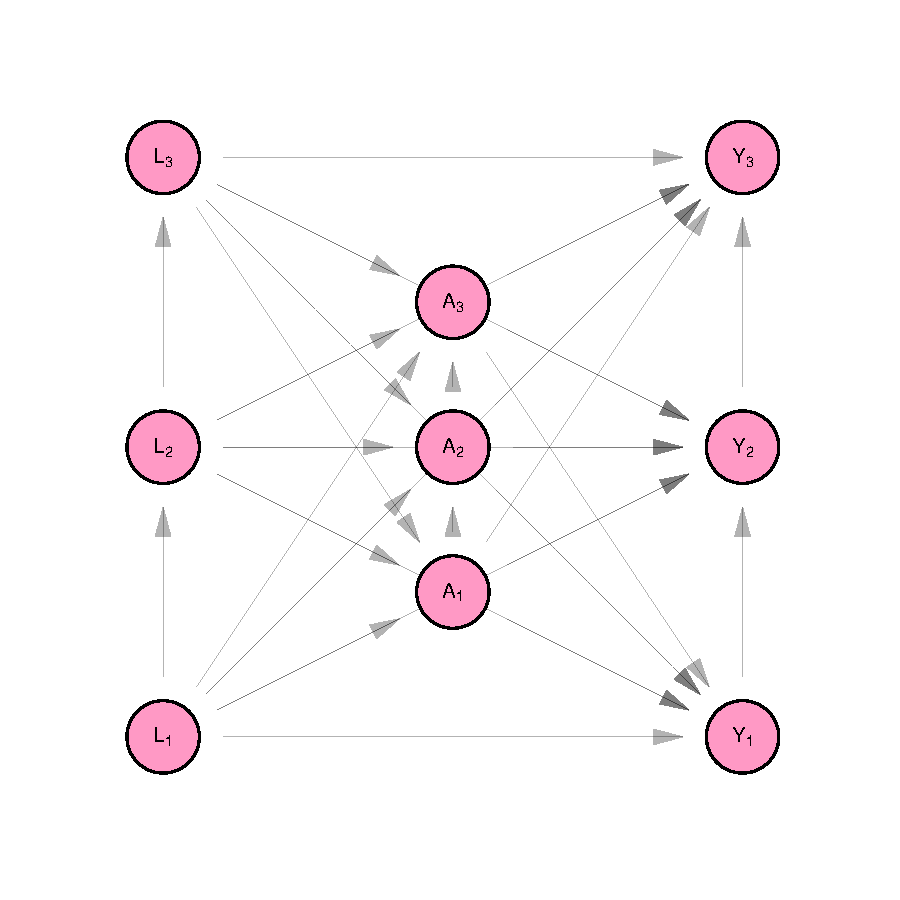
\includegraphics{C_sscan3_causal_interpretation/C__sscan3_causal_interpretation_files/figure-pdf/fig-fullly-connected-dag-1.pdf}

}

\caption{\label{fig-fullly-connected-dag}Fully connected causal DAG}

\end{figure}

\begin{equation}\protect\hypertarget{eq-fullly-connected-dag}{}{
\begin{aligned}
L_1 &= f_{L_1}(U_{L_1}) \\
L_2 &= f_{L_2}(U_{L_2}, L_1) \\
L_3 &= f_{L_3}(U_{L_3}, L_1, L_2 ) \\
A_1 &= f_{A_1}(U_{A_1}, L_1, L_2, L_3) \\
A_2 &= f_{A_2}(U_{A_2}, L_1, L_2, L_3, A_1) \\
A_3 &= f_{A_3}(U_{A_3}, L_1, L_2, L_3, A_1, A_2) \\
Y_1 &= f_{Y_1}(U_{Y_1}, L_1, L_2, L_3, A_1, A_2, A_3) \\
Y_2 &= f_{Y_2}(U_{Y_2}, L_1, L_2, L_3, A_1, A_2, A_3, Y_1) \\
Y_3 &= f_{Y_3}(U_{Y_3}, L_1, L_2, L_3, A_1, A_2, A_3, Y_1, Y_2) \\
\end{aligned}
}\label{eq-fullly-connected-dag}\end{equation}

But the most flexible model is not the most useful one. To fully
characterize this system using observed data, we would need to estimate
9 functions using one observation of the 9-dimensional joint
distribution that gave rise to the participants' observations.
Recruiting an additional person to the study would not ease this
problem; it would add three new equations to the model and we would end
up with a similar problem than the one we began with. We would have to
estimate 12 functions using one observation of a 12-dimensional joint
distribution.

Epidemiologists take several approaches to to simplify this system of
equations by making assumptions that leave us with fewer functions to
estimate and more observations per function. These assumptions are
called model restrictions because they restrict the number of possible
distributions that could be represented by the model.

For instance, if we add the restriction to the model shown above that
all the measures are independent (or equivalently, that the DAG has no
arrows), the resulting model would not be able to represent data from a
causal system where some of the measures are correlated. By adding the
restriction of independence, we would be eliminating the correlated data
distribution from consideration as a possibility for how the data we are
modelling are truly distributed.

In the next few sections, we will discuss the restrictions made under
classic causal inference, network causal inference, and the SSNAC
framework. In each case, simplifying the system of equations equates to
deleting some of the arrows in the DAG shown in
Figure~\ref{fig-fullly-connected-dag} (or equivalently, deleting some
arguments from the functions in Equation~\ref{eq-fullly-connected-dag}),
or assuming that some of the functions in the system are similar to each
other in some way.

\hypertarget{sec-assumptions-classic}{%
\subsection{Assumptions}\label{sec-assumptions-classic}}

Under classic causal inference, we assume that observations are
independent and identically distributed. We review these assumptions,
naming them slightly differently for the purpose of comparing them with
the assumptions made in subsequent sections. In each case, we divide
assumptions up into \emph{independence assumptions} (assumptions that
delete arrows from the DAG) and \emph{homogeneity assumptions}
(assumptions that simplify the system of structural equations).

\hypertarget{independence}{%
\subsubsection{Independence}\label{independence}}

\hypertarget{no-spillover}{%
\paragraph{No spillover}\label{no-spillover}}

Under classic causal inference, we make the assumption of no spillover -
that measurements taken across participants at the same time
(e.g.~\(L_1\), \(L_2\), and \(L_3\)) are independent of each other given
all prior measures. i.e.

\[
\begin{aligned}
L_1 \perp L_2 \\
L_2 \perp L_3 \\
L_1 \perp L_3 
\end{aligned}
\]

\[
\begin{aligned}
A_1 \perp A_2 | L_1, L_2, L_3\\
A_2 \perp A_3 | L_1, L_2, L_3 \\
A_1 \perp A_3 | L_1, L_2, L_3 
\end{aligned}
\]

\[
\begin{aligned}
Y_1 \perp Y_2 | L_1, L_2, L_3, A_1, A_2, A_3\\
Y_2 \perp Y_3 | L_1, L_2, L_3, A_1, A_2, A_3 \\
Y_1 \perp Y_3 | L_1, L_2, L_3, A_1, A_2, A_3 
\end{aligned}
\]

This is shown in Figure~\ref{fig-no-spillover-dag}, as the removal of
arrows that connected the \(L_i\)'s, \(A_i\)'s and \(Y_i\)'s. In
Equation~\ref{eq-no-spillover-dag}, the \(L_i\)'s are not functions of
each other, the \(A_i\)'s are not functions of each other, and the
\(Y_i\)'s are not functions of each other. i.e.~Given all the
measurements taken prior to a set of contemporaneous measures, the
contemporaneous measures are independent. (This follows from the
independence of the error terms \(U_{L_i}\), the error terms
\(U_{A_i}\), and the error terms \(U_{Y_i}\) across observations \(i\).)

\begin{Shaded}
\begin{Highlighting}[]
\FunctionTok{make\_dag}\NormalTok{(}\StringTok{"full\_interference"}\NormalTok{)      }\SpecialCharTok{|\textgreater{}} 
  \FunctionTok{plot\_swig}\NormalTok{(}\AttributeTok{node\_radius =} \FloatTok{0.2}\NormalTok{) }\SpecialCharTok{+} 
  \FunctionTok{scale\_fill\_mpxnyc}\NormalTok{(}\AttributeTok{labels =} \FunctionTok{c}\NormalTok{(}\StringTok{"h"}\NormalTok{), }\AttributeTok{option =} \StringTok{"light"}\NormalTok{) }\SpecialCharTok{+}
  \FunctionTok{theme\_mpxnyc\_blank}\NormalTok{()}
\end{Highlighting}
\end{Shaded}

\begin{figure}[H]

{\centering 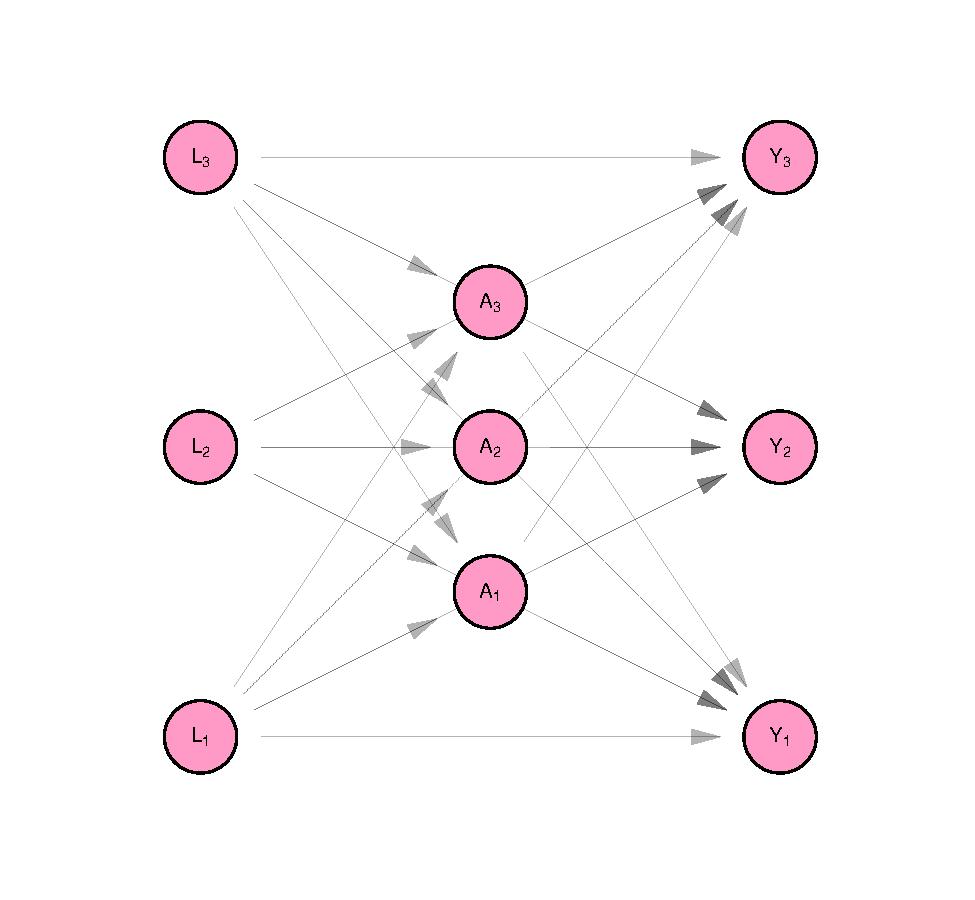
\includegraphics{C_sscan3_causal_interpretation/C__sscan3_causal_interpretation_files/figure-pdf/fig-no-spillover-dag-1.pdf}

}

\caption{\label{fig-no-spillover-dag}Causal DAG with no spillover}

\end{figure}

\begin{equation}\protect\hypertarget{eq-no-spillover-dag}{}{
\begin{aligned}
L_1 &= f_{L_1}(U_{L_1}) \\
L_2 &= f_{L_2}(U_{L_2}) \\
L_3 &= f_{L_3}(U_{L_3} ) \\
A_1 &= f_{A_1}(U_{A_1}, L_1, L_2, L_3) \\
A_2 &= f_{A_2}(U_{A_2}, L_1, L_2, L_3) \\
A_3 &= f_{A_3}(U_{A_3}, L_1, L_2, L_3) \\
Y_1 &= f_{Y_1}(U_{Y_1}, L_1, L_2, L_3, A_1, A_2, A_3) \\
Y_2 &= f_{Y_2}(U_{Y_2}, L_1, L_2, L_3, A_1, A_2, A_3) \\
Y_3 &= f_{Y_3}(U_{Y_3}, L_1, L_2, L_3, A_1, A_2, A_3) \\
\end{aligned}
}\label{eq-no-spillover-dag}\end{equation}

\hypertarget{no-interference}{%
\paragraph{No interference}\label{no-interference}}

Classic causal inference makes the assumption of no interference.
i.e.~We assume that measurements made across participants, but not at
the same time are independent of each other. This is shown as the
absence of arrows that point from the \(L_i\)'s to \(A_j\)'s, the
\(L_i\)'s to the \(Y_j\)'s and the \(A_i\)'s to the \(Y_j\) for
participants \(i\neq j\) (see Figure~\ref{fig-independence-dag}).

This allows us to simplify the structural equation model so that each
participant's measures are a function of only measures taken on them.

\[
\begin{aligned}
L_1 &= f_{L_1}( U_{L_1}) \\
L_2 &= f_{L_2}( U_{L_2}) \\
L_3 &= f_{L_3}( U_{L_3}) \\
A_1 &= f_{A_1}( U_{A_1}, L_1) \\
A_2 &= f_{A_2}( U_{A_2}, L_2) \\
A_3 &= f_{A_3}( U_{A_3}, L_3) \\
Y_1 &= f_{Y_1}( U_{Y_1}, L_1, A_1 ) \\
Y_2 &= f_{Y_2}( U_{Y_2}, L_2, A_2 ) \\
Y_3 &= f_{Y_3}( U_{Y_3}, L_3, A_3 ) \\
\end{aligned}
\]

\hypertarget{homogeneity}{%
\subsubsection{Homogeneity}\label{homogeneity}}

\hypertarget{identical-distribution}{%
\paragraph{Identical distribution}\label{identical-distribution}}

Finally, we see above that the functions that generate observations
\(L_i\) are similar in structure to each other, as are the the functions
that generate \(A_i\)'s and \(Y_i\)s. We make the homogeneity assumption
that the functions are identical to each other.

\[
\begin{aligned}
 f_L &= f_{L_1} = f_{L_2} = f_{L_3} \\
 f_A &= f_{A_1} = f_{A_2} = f_{A_3} \\
 f_Y &= f_{Y_1} = f_{Y_2} = f_{Y_3}  \\
\end{aligned}
\]

\hypertarget{identification}{%
\subsubsection{Identification}\label{identification}}

\hypertarget{positivity}{%
\paragraph{Positivity}\label{positivity}}

We assume that for all \(i\)

\[
0 < P[A_i =1 | L_i] < 1
\]

\hypertarget{model}{%
\subsection{Model}\label{model}}

\hypertarget{observed-data}{%
\subsubsection{Observed data}\label{observed-data}}

The homogeneity and indepdndence assumptions allow us to re-write the
structural equation model dropping the person subscript from the
equations. The model simplifies into one for three measures each taken
on one person, rather than a model for 9 measures taken on 3 people.
Since the measures on each person are identically distributed, this
model can be used three times to separately generate the measures for
\emph{Person 1}, \emph{Person 2}, and \emph{Person 3}. By contrast, the
original model produced measures for all three people at one go.

Figure~\ref{fig-independence-dag} and Equation~\ref{eq-independence-dag}
show the resulting non-parametric structural equation model for our
data, if we analyse it under classic causal inference. As a consequence
of the assumptions stated in Section~\ref{sec-assumptions-classic}, we
can represent the model using three equations rather than 9. We retain
the person subscript on the random variables in
Figure~\ref{fig-independence-dag} and we keep all 9 nodes in the DAG on
Equation~\ref{eq-independence-dag}. This is to remind us that though our
model is for one person, our purpose was always to infer something about
the sample of three people.

\begin{Shaded}
\begin{Highlighting}[]
\FunctionTok{make\_dag}\NormalTok{(}\StringTok{"independence"}\NormalTok{) }\SpecialCharTok{|\textgreater{}} 
  \FunctionTok{plot\_swig}\NormalTok{(}\AttributeTok{node\_radius =} \FloatTok{0.2}\NormalTok{) }\SpecialCharTok{+} 
  \FunctionTok{scale\_fill\_mpxnyc}\NormalTok{(}\AttributeTok{option =} \StringTok{"light"}\NormalTok{) }\SpecialCharTok{+} 
  \FunctionTok{theme\_mpxnyc\_blank}\NormalTok{()}
\end{Highlighting}
\end{Shaded}

\begin{figure}[H]

{\centering 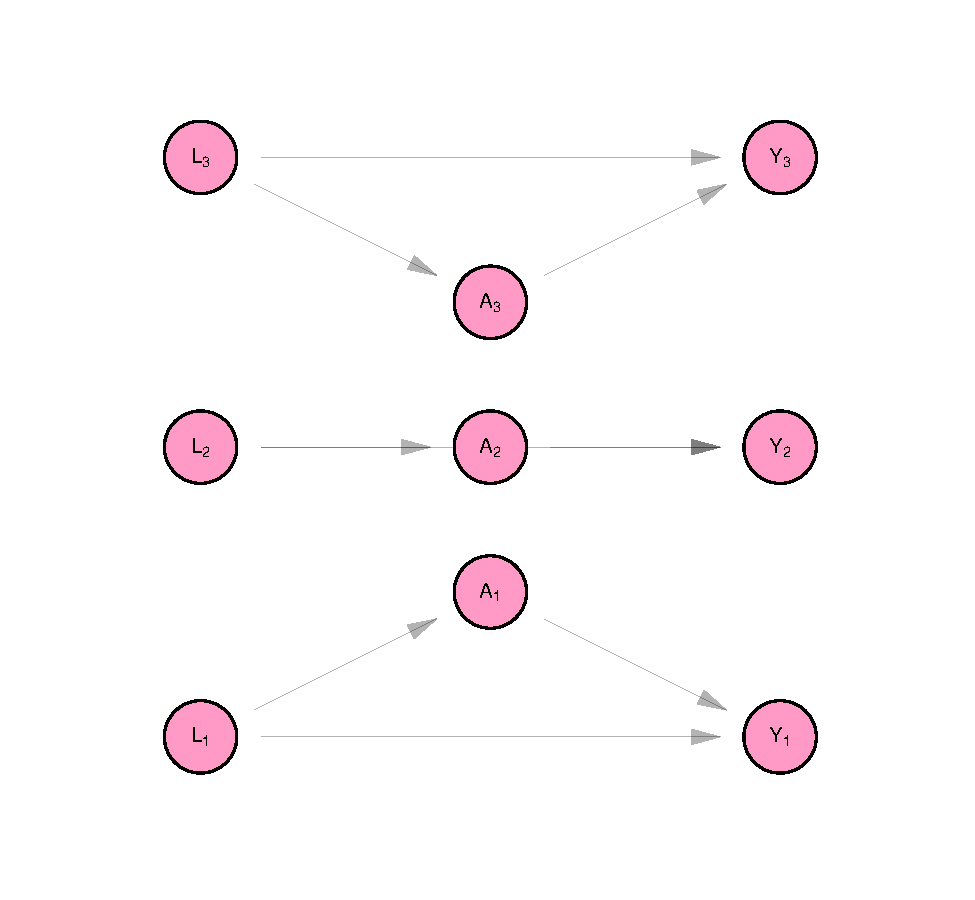
\includegraphics{C_sscan3_causal_interpretation/C__sscan3_causal_interpretation_files/figure-pdf/fig-independence-dag-1.pdf}

}

\caption{\label{fig-independence-dag}Causal DAG with no interference or
spillover}

\end{figure}

\begin{equation}\protect\hypertarget{eq-independence-dag}{}{
\begin{aligned}
L_i &= f_{L}( U_{L_i}) \\
A_i &= f_{A}( U_{A_i}, L_i) \\
Y_i &= f_{Y}( U_{Y_i}, L_i, A_i) \\
\end{aligned}
}\label{eq-independence-dag}\end{equation}

\hypertarget{counterfactual-data}{%
\subsubsection{Counterfactual data}\label{counterfactual-data}}

We define counterfactual outcomes \(Y_1^{(a_1)}\), \(Y_2^{(a_2)}\), and
\(Y_3^{(a_3)}\), which represent the level of job opportunities,
\emph{Persons 1}, \emph{2}, and \emph{3}, would have if we set their
dress to level \(a_1\), \(a_2\), and \(a_3\), respectively. Then the
model for counterfactual variables is given by
Equation~\ref{eq-independence-swig}.

It is represented using the Single World Intervention Graph (SWIG)
pictured in Figure~\ref{fig-independence-swig}. A SWIG represents a
structural equation model where some of the equations are superseded by
the value assigned by the experimenter. For so-called ``treatment
variables'', the diagram separates the value of the variable as it would
have been observed with no intervention (\(A_i\)) from the value that as
it will be used in subsequent equations (\(a_i\)) as a result of the
experimenter's intervention.

Note that because of the assumption of no interference and no spillover,
each counterfactual outcome is a function only of the treatment value of
the same individual.

\begin{Shaded}
\begin{Highlighting}[]
\FunctionTok{make\_swig}\NormalTok{(}\StringTok{"independence"}\NormalTok{)      }\SpecialCharTok{|\textgreater{}} 
  \FunctionTok{plot\_swig}\NormalTok{(}\AttributeTok{node\_radius =} \FloatTok{0.2}\NormalTok{) }\SpecialCharTok{+} 
  \FunctionTok{scale\_fill\_mpxnyc}\NormalTok{(}\AttributeTok{option =} \StringTok{"light"}\NormalTok{) }\SpecialCharTok{+}
  \FunctionTok{theme\_mpxnyc\_blank}\NormalTok{()}
\end{Highlighting}
\end{Shaded}

\begin{figure}[H]

{\centering 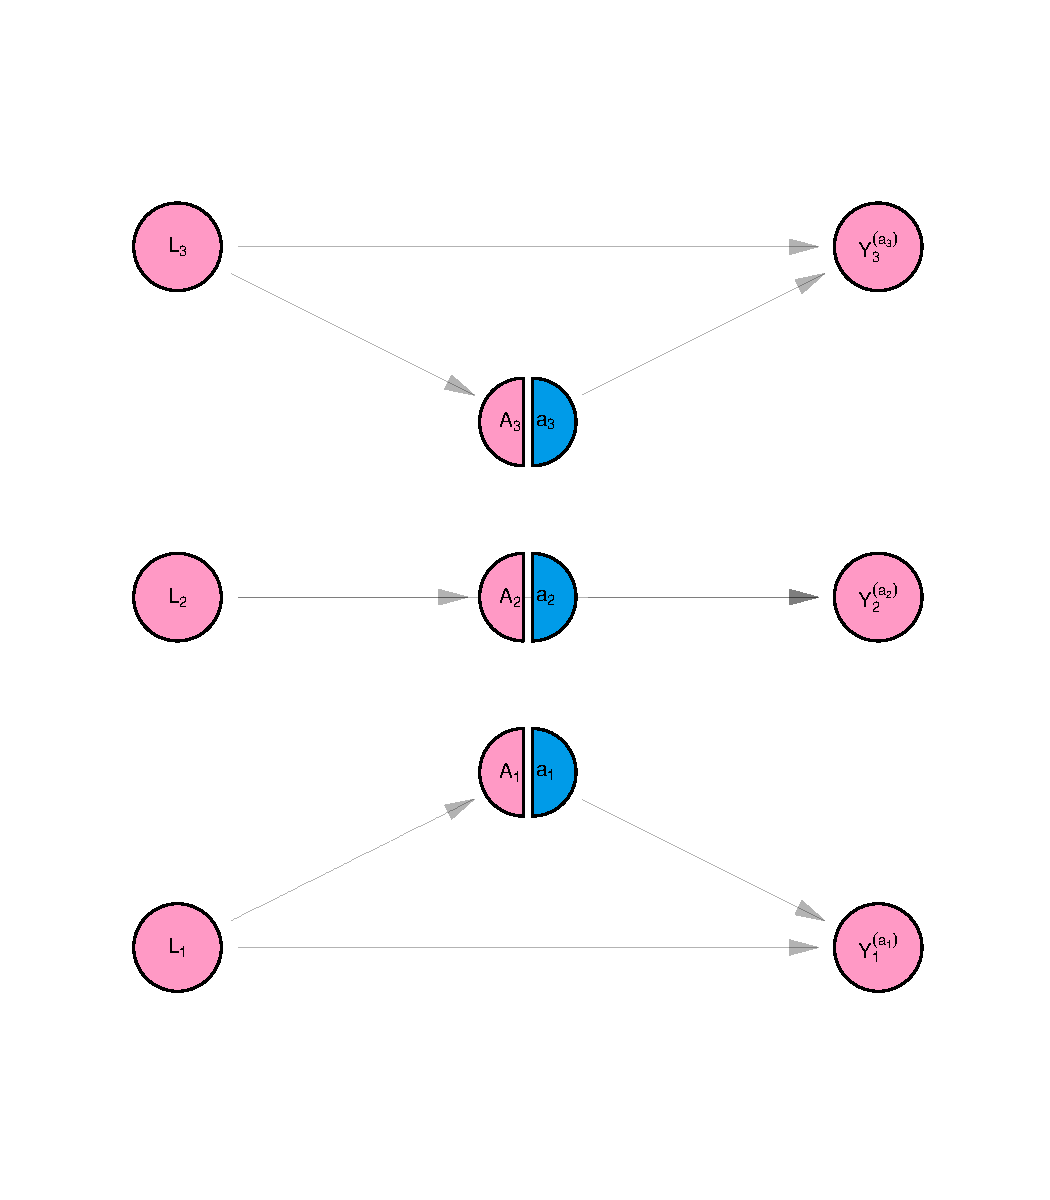
\includegraphics{C_sscan3_causal_interpretation/C__sscan3_causal_interpretation_files/figure-pdf/fig-independence-swig-1.pdf}

}

\caption{\label{fig-independence-swig}SWIG with no interference or
spillover}

\end{figure}

\begin{equation}\protect\hypertarget{eq-independence-swig}{}{
\begin{aligned}
L_i &= f_{L}( U_{L_i}                       ) \\
A_i &= f_{A}( U_{A_i}, L_i) \\
Y_i^{(a_i)} &= f_{Y}(U_{Y_i} , L_i, a_i) \\
\end{aligned}
}\label{eq-independence-swig}\end{equation}

\hypertarget{estimates}{%
\subsection{Estimates}\label{estimates}}

\hypertarget{estimands}{%
\subsubsection{Estimands}\label{estimands}}

We are interested in whether changing how formally someone dresses would
change their level of job offers, on average, in our population. To
determine the answer, we will compare the average counterfactual outcome
of job opportunities for formal dress to the average counterfactual
outcome of job opportunities for non-formal dress. i.e.~We will make the
following comparison.

\[
\begin{aligned}
E \left[ \frac{1}{n} \sum_i Y_i^{(a=1)} - Y_i^{(a=0)} \right]
\end{aligned}
\]

\hypertarget{identification-1}{%
\subsubsection{Identification}\label{identification-1}}

Once we have specified the hypothetical quantities from our thought
experiment, we ``identify'' them, meaning write them in terms of the
observed rather than counterfactual data. It is sufficient to identify
the quantity:

\[
E \left[ \frac{1}{n} \sum_i E[Y_i^{(a)} | L_i] \right] \\
\]

The inner expectation can be re-written as follows:

\[
\begin{aligned}
 E[ Y_i^{(a)} | L_i  ]   &=  E[  Y_i^{(a)} | L_i  , A_i = a ]   \\
                                &=  E[ f_{Y}(U_{Y_i} , l_i, a) | L_i  , A_i = a ]   \\
                                &=  E[ Y_i | L_i , A_i = a, ]   \\
\end{aligned}
\]

\begin{itemize}
\item
  In the first line, we use the fact that since it is constant, the
  value of dress set by the experimenter \(a\) is independent of the
  observed value of dress \(A_i\) for each person \(i\).
\item
  In the second line, we use the no spillover and no interference
  assumptions - person \(i\)'s values (including counterfactual values)
  are independent of any measures not taken on person \(i\).
\item
  In the third line we substitute \(Y_i^{(a)}\) for the structural
  equation that produces that variable, according to the model in
  Equation~\ref{eq-independence-swig}.
\item
  In the fourth line, we substitute the structural equation for the
  observed value \(Y_i\) according to the model in
  Equation~\ref{eq-independence-dag}.
\end{itemize}

(Note that the function \(f_y\) in Equation~\ref{eq-independence-swig}
is identical to the function \(f_y\) in
Equation~\ref{eq-independence-dag}. The error term for person \(i\),
\(U_{Y_i}\) has the same value in both the counterfactual and
observational models, as does the value of \(l_i\). As a result,
\(f_{Y}(U_{Y_i} , l_i, a)\) is equal to the observed value as well as
the counterfactual value for participants \(i\) if \(A_i = a\)).

The functional we have to estimate from data is the following.

\[
E[ \frac{1}{n} \sum_i{E[ Y_i | L_i , A_i = a ]}  ] 
\]

We can evaluate the inner expectation (with respect to \(Y_i\)) by
taking averages across sub groups in the study dataset. Then we have a
function of random vector \(\mathbf{L}\) to evaluate in the outer
expectation.

\[
\frac{\sum_i E[ Y_i | L_i = l_i, A_i = a ]I_{\{ x = a\}}(a_i)}{\sum_i I_{\{ x = a\}}(a_i) }
\]

\hypertarget{discussion}{%
\subsection{Discussion}\label{discussion}}

\hypertarget{consistency}{%
\subsubsection{Consistency}\label{consistency}}

\begin{itemize}
\tightlist
\item
  Assumption that for a given individual observed and counterfactual
  distributions use the same structural equations and error term
\item
  That means his counterfactual value under the treatment level he
  received is going to be equal to his observed value
\item
  This is the assumption that allows us to substitute the observed value
  in the identification strategy above
\end{itemize}

\hypertarget{positivity-1}{%
\subsubsection{Positivity}\label{positivity-1}}

\begin{itemize}
\tightlist
\item
  Assumption that each combination of treatments and covariates has a
  non-zero chance of developing the outcome
\end{itemize}

\hypertarget{exchangeability}{%
\subsubsection{Exchangeability}\label{exchangeability}}

\begin{itemize}
\tightlist
\item
  We have not misspecified the DAG
\end{itemize}

\hypertarget{reflection-questions}{%
\subsection*{Reflection questions}\label{reflection-questions}}
\addcontentsline{toc}{subsection}{Reflection questions}

Using the structural equations:

\begin{enumerate}
\def\labelenumi{\arabic{enumi}.}
\item
  Show that independence does not hold in the model defined by
  Equation~\ref{eq-fullly-connected-dag}.
\item
  Show that independence holds in Equation~\ref{eq-independence-dag}.
\item
  Show that the causal estimand in
  Section~\ref{sec-classic-causal-inference} is equivalent to the usual
  definition of average causal effect (ACE)
\item
  Show that the causal estimate in
  Section~\ref{sec-classic-causal-inference} is equivalent to the usual
  definition of the g-formula.
\item
  How is the SUTVA or consistency assumption encoded in this model?
\end{enumerate}

\hypertarget{sec-network-causal-inference}{%
\section{Network causal inference}\label{sec-network-causal-inference}}

\hypertarget{example-2-marriage-dress-and-jobs}{%
\subsection*{Example 2: Marriage, Dress, and
Jobs}\label{example-2-marriage-dress-and-jobs}}
\addcontentsline{toc}{subsection}{Example 2: Marriage, Dress, and Jobs}

We mentioned that in our study sample that \emph{Person 1} and
\emph{Person 2} are married to each other, and \emph{Person 1} and
\emph{Person 3} are new colleagues. In the causal system connecting
their job status, dress and job offers, an argument could be made that
\emph{Person 1}'s job status affects \emph{Person 2}'s dress, since they
pool their salaries as a married couple. It could also be argued that
\emph{Person 1}'s job status affects \emph{Person 2}'s job opportunities
if having a job brings the married couple into contact with other
married couples who are connected to job markets.

Finally, we could argue that \emph{Person 1}'s dress affects
\emph{Person 2}'s job opportunities if some aspect of the reputation
\emph{Person 2} enjoys among potential colleagues derives from
\emph{Person 1}'s current job in that market. Symmetrically,
\emph{Person 2}'s current job could also potentially affect \emph{Person
1's} job opportunities.

But what about the relationship between \emph{Person 1} and \emph{Person
3}? How does that shape the measurements of either person? We can
imagine that the dress of a newly acquainted colleague would not affect
the dress and job opportunities of her colleague. Whereas \emph{Person
1} and \emph{Person 2} are causally related, \emph{Person 1} and
\emph{Person 3} are not; their relationship is irrelevant to the causal
system under investigation. \emph{Person 2} and \emph{Person 3} do not
affect each other since they have no relationship at all.

Before specifying a model that can accommodate the interdependence
between \emph{Person's 1} and \emph{2}, we outline some definitions
which we will need for the independence and homogeneity assumptions that
define the network causal inference approach to causal analysis. Loosely
following Aronow and Samii (2017), we use the idea of exposure mappings
to express these assumptions.

\hypertarget{graphs}{%
\subsection*{Graphs}\label{graphs}}
\addcontentsline{toc}{subsection}{Graphs}

We define graph \(\mathscr{G}(\mathscr{N}, \sim)\) as an ordered pair
whose first entry is a set \(\mathscr{N}\) containing nodes, and second
entry a relation \(\sim\) which indicates edges between nodes
(\(i \sim j\) means ``\(i\) is connected to \(j\) in \(\mathscr{G}\)'',
for instance). There are \(n = |\mathscr{N}|\) nodes, which each
represent individuals in the study sample. We further define
\(\mathscr{N_i} = \{j \in \mathscr{N}: i \sim j\}\) as the ``network
exposure units'' for person \(i\). The set contains the names of all the
nodes \(i\) is connected to. Define \(\mathbf{X}_{\mathscr{N_i}}\) as
the sub-vector of \(\mathbf{X}\) which contains entries related to
person \(i\)'s network exposure units.

\hypertarget{exposure-mappings}{%
\subsection*{Exposure mappings}\label{exposure-mappings}}
\addcontentsline{toc}{subsection}{Exposure mappings}

Say we have a non-parametric structural equation model of
\(n\)-dimensional random vectors \(\mathbf{X}_t \in \{0,1\}^n\),
\(t \in [1,k]\), which precede random vector \(\mathbf{Y}\). \(f_{Y_i}\)
is the structural equation for \(Y_i\), and \(U_{Y_i}\) the error term
for that equation. We define the ``exposure mapping for \(Y_i\)'' as the
function

\[
g_i: \{0,1\}^{n\times k} \times\mathscr{N} \rightarrow \mathbf{R}^{2k}
\]

such that

\[
Y_i = f_{Y_i}(g_i(\mathbf{X}_1,  ..., \mathbf{X}_k, i), U_{Y_i})
\]

\hypertarget{definition-1-loyalty}{%
\subsubsection{Definition 1: Loyalty}\label{definition-1-loyalty}}

We say an exposure mapping \(g_{i}\) is loyal to graph \(\mathscr{G}\)
if for any \(\mathbf{X},\mathbf{X}' \in \mathbf{R}^n\)

\[
\begin{equation}
\mathbf{X}_{\mathscr{N}_i} = \mathbf{X'}_{\mathscr{N}_i} \text{ and } X_i = X'_i\\
\implies \\
g_{i}(\mathbf{X}, i) = g_{i}(\mathbf{X'}, i) 
\end{equation}
\]

\hypertarget{definition-2-separability}{%
\subsubsection{Definition 2:
Separability}\label{definition-2-separability}}

We say exposure mapping \(g_i\) is separable if it can be re-written as
the vector-valued function

\[
g_i(\mathbf{X}_{1}, ..., \mathbf{X}_{k}, i) = \begin{pmatrix} 
g_{0i}(\mathbf{X}_{1}, ..., \mathbf{X}_{k},  i)  \\ 
g_{1i}(\mathbf{X}_{1},  i) \\
... \\  
g_{ki}(\mathbf{X}_{k},  i) 
\end{pmatrix}
\]

Where for \(g_{0i}\) is a vector-valued function of \(X_{ti}\) for
\(t \in [1,k]\) and each \(g_{ti}\) is a real-valued function.

\hypertarget{definition-3-symmetry}{%
\subsubsection{Definition 3: Symmetry}\label{definition-3-symmetry}}

For some \(t \in [1,K]\) and \(i \in \mathscr{N}\), we say \(g_{ti}\) is
symmetric with respect to graph \(\mathscr{G}\) if for any
\(\mathbf{X},\mathbf{X}' \in \mathbf{R}^n\) and permutation matrix
\(\mathbf{M}\) (conformable square matrix whose row and column margins
all equal 1):

\[
\begin{equation}
\mathbf{X}_{\mathscr{N}_i} = \mathbf{M} \mathbf{X'}_{\mathscr{N}_i}  \\
\implies \\
g_{ti}(\mathbf{X}, i) = g_{ti}(\mathbf{X'}, i) 
\end{equation}
\]

If \(g_{ti}\) is symmetric with respect to \(\mathscr{G}\) we say it is
a ``network exposure mapping for \(Y_i\) with respect to
\(\mathbf{X}_t\) in \(\mathscr{G}\)''. The value of the function is
called the ``network exposure value\ldots{}''

\hypertarget{definition-4-positional-invariance}{%
\subsubsection{Definition 4: Positional
invariance}\label{definition-4-positional-invariance}}

We say an network exposure mapping \(g_{ti}\) is invariant to its
position in the network if

\[
g_{ti} = g_{tj} = g_t \text{ for all } i,j \in \mathscr{N} 
\]

\hypertarget{definition-5-boundedness}{%
\subsubsection{Definition 5:
Boundedness}\label{definition-5-boundedness}}

We say that a network exposure mapping \(g_{ti}\) is bounded if all
possible network exposure values are contained by a finite set
\(\mathbf{D}\)

\[
g_{ti}(\mathbf{X}_t, i) \in \mathbf{D} 
\]

and \(|\mathbf{D}| < c\) for some constant \(c\).

\hypertarget{comments}{%
\subsubsection{Comments}\label{comments}}

These definitions will be used in the next section to develop a model
for inference under causal interference. The first assumption can be
stated in graphic terms - it implies certain conditional independencies
that can be encoded in a DAG by the removal and addition of arrows
between nodes. The DAG in question would represent all the observational
units rather than one (a typical) observation unit.

The following four assumptions are crucial to define here because they
are not possible to encode in the aforementioned DAG. We will use these
to impose homogeneity restrictions on the DAG that enable us to apply
statistical inference methods that are usually thought to require
independence of observations. We will make a weaker assumption - that of
``no spillover'', impose homogeneity restrictions, and apply familiar
methods such as generalized linear models to reason about network
phenomena.

It is useful to point out that the symmetry of a network exposure
mapping \(g_{ti}\) implies that the only thing that matters for the
contribution of alters to \(Y_i\) is the count of alters for which
\(X_t = 1\). The positional invariance of \(g_{ti}\) means that what
ever the function is that relates these counts to the outcome \(Y_i\) is
the same across observational units. Boundedness limits the number of
distinct values that \(g_{ti}\) can take because each distinct value
constitutes a treatment level whose counterfactual we have to model. As
we will see, the assumption of boundedness limits the number of
counterfactuals.

Under network causal inference, boundedness can obtain in three
different ways. First, it could be as a result of restrictions on the
structure of the underlying network. It could be the case that in the
network of interest, there is an upper bound on node degree. For
example, if the only relationships of interest between individual
participants were marriages, each node would have a degree of either 0
or 1, meaning the count of alters \(X_{tj} = 1, j \in N_i\) is either
zero or one. The second way boundedness might obtain is via restrictions
of the value of \(\mathbf{X}_t\). It might be the case, for instance,
that the count of \(i\)'s for which \(X_{ti}=1\) is very low, then on
average, the count of alters for which \(X_{tj} = 1, j \in N_i\) will
also be low. Finally, boundedness could obtain as a result of the
functional form of \(g_t\) itself.

This might happen if \(g_t\) models a network exposure which has a
ceiling effect in its dose-response curve with the outcome of interest
\(Y_i\). For example, if \(X_t\) indicates ownership of a car, and
\(\mathscr{G}\) encodes close friendships, \(g_t\) would be a network
exposure mapping which tells us how each additional friend who has a car
shifts the outcome of interest. For most applications, its likely that
beyond some number of friends (say 5) who have a car, an additional
friend who gets a car will not change the outcome under investigation.

Finally, we should note that under classical causal inference
\(g_t = c \in \mathbf{R}\) for \(t \in [1,k]\). Exposure models are
trivially loyal to the empty graph, so the network exposure mappings are
trivially separable, positionally invariant, and bounded.

\hypertarget{assumptions}{%
\subsection{Assumptions}\label{assumptions}}

\hypertarget{independence-assumptions}{%
\subsubsection{Independence
assumptions}\label{independence-assumptions}}

\hypertarget{no-spillover-1}{%
\paragraph{No spillover}\label{no-spillover-1}}

Under network causal inference, we make the assumption of no spillover -
that measurements taken across participants at the same time
(e.g.~\(L_1\), \(L_2\), and \(L_3\)) are independent of each other given
all prior measures.

This is shown in Figure~\ref{fig-interference-dag}, as the removal of
arrows that connected the \(L_i\)'s, \(A_i\)'s and \(Y_i\)'s in
Figure~\ref{fig-fullly-connected-dag}. In
Equation~\ref{eq-interference-dag}, the \(L_i\)'s are not functions of
each other, the \(A_i\)'s are not functions of each other, and the
\(Y_i\)'s are not functions of each other. This implies that given all
the measurements taken prior to a set of contemporaneous measures, the
contemporaneous measures are independent.

\hypertarget{network-interference}{%
\paragraph{Network interference}\label{network-interference}}

\begin{Shaded}
\begin{Highlighting}[]
\FunctionTok{make\_dag}\NormalTok{(}\StringTok{"network\_interference"}\NormalTok{)   }\SpecialCharTok{|\textgreater{}} 
  \FunctionTok{plot\_swig}\NormalTok{(}\AttributeTok{node\_radius =} \FloatTok{0.2}\NormalTok{) }\SpecialCharTok{+} 
  \FunctionTok{scale\_fill\_mpxnyc}\NormalTok{(}\AttributeTok{option =} \StringTok{"light"}\NormalTok{) }\SpecialCharTok{+}
  \FunctionTok{theme\_mpxnyc\_blank}\NormalTok{()}
\end{Highlighting}
\end{Shaded}

\begin{figure}[H]

{\centering 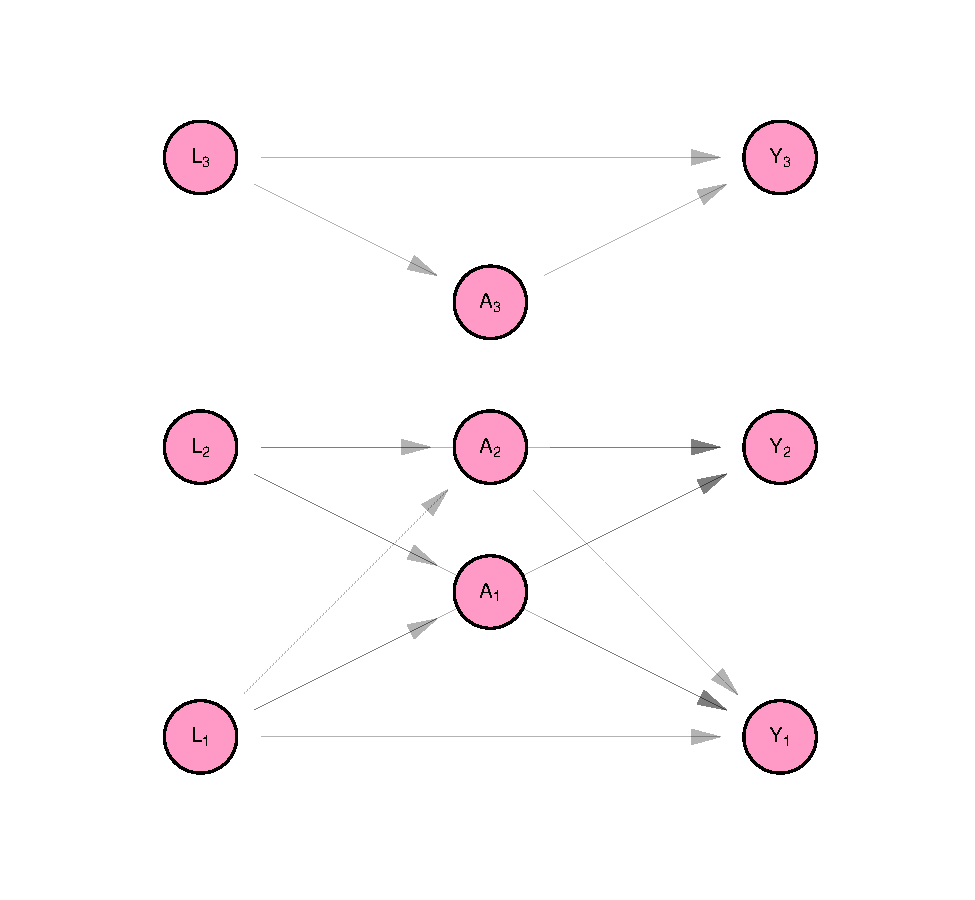
\includegraphics{C_sscan3_causal_interpretation/C__sscan3_causal_interpretation_files/figure-pdf/fig-interference-dag-1.pdf}

}

\caption{\label{fig-interference-dag}Causal DAG with network
interference}

\end{figure}

\begin{equation}\protect\hypertarget{eq-interference-dag}{}{
\begin{aligned}
L_1 &= f_{L_1}(U_{L_1}) \\
L_2 &= f_{L_2}(U_{L_2}) \\
L_3 &= f_{L_3}(U_{L_3} ) \\
A_1 &= f_{A_1}(U_{A_1}, L_1, L_2) \\
A_2 &= f_{A_2}(U_{A_2}, L_1, L_2) \\
A_3 &= f_{A_3}(U_{A_3}, L_3) \\
Y_1 &= f_{Y_1}(U_{Y_1}, L_1, L_2, A_1, A_2) \\
Y_2 &= f_{Y_2}(U_{Y_2}, L_1, L_2, A_1, A_2) \\
Y_3 &= f_{Y_3}(U_{Y_3}, L_3,  A_3) \\
\end{aligned}
}\label{eq-interference-dag}\end{equation}

Under network causal inference, we make the assumption that interference
respects some mapping between individuals - a mapping given by a graph.
In Figure~\ref{fig-interference-dag}, based on their relationships with
one another, \emph{Person 1}'s measures are connected with \emph{Person
2}'s, and neither are connected with \emph{Person 3}. See Aronow and
Samii (2017).

Saying a structural equation model or a DAG shows network interference
is equivalent to saying the exposure mapping for each variable in the
DAG is loyal to graph \(\mathscr{G}\) which encodes the causally
relevant relationships between observational units in the sample. In
this example

\[
\mathscr{G}(\{\text{Person 1, Person 2, Person 3}\}, \{\text{Person 1} \sim \text{Person 2}\})
\]

\hypertarget{homogeneity-assumptions}{%
\subsubsection{Homogeneity assumptions}\label{homogeneity-assumptions}}

\hypertarget{homogenous-interference}{%
\paragraph{Homogenous interference}\label{homogenous-interference}}

\hypertarget{separability}{%
\subparagraph{Separability}\label{separability}}

We assume that the exposure mapping for each variable in the structural
model is separable. i.e.~We define \(g_{A_i}\), \(h_{Y_i}\), and
\(g_{Y_i}\) as network exposure mappings for \(A_i\) with respect to
\(\mathbf{L}\), for \(Y_i\) with respect to \(\mathbf{A}\), and for
\(Y_i\) with respect to \(\mathbf{L}\). Seperability allows us to write
the model as follows:

\[
\begin{aligned}
L_1 &= f_{L_1}(U_{L_1}) \\
L_2 &= f_{L_2}(U_{L_2}) \\
L_3 &= f_{L_3}(U_{L_3} ) \\
A_1 &= f_{A_1}(U_{A_1}, L_1, g_{A_1}(\mathbf{L}, \{2\})) \\
A_2 &= f_{A_2}(U_{A_2}, L_2, g_{A_2}(\mathbf{L}, \{1\})) \\
A_3 &= f_{A_3}(U_{A_3}, L_3, g_{A_3}(\mathbf{L}, \{\})) \\
Y_1 &= f_{Y_1}(U_{Y_1}, L_1, A_1, g_{Y_1}(\mathbf{L}, \{2\}), h_{Y_1}(\mathbf{A}, \{2\})) \\
Y_2 &= f_{Y_2}(U_{Y_2}, L_2, A_2, g_{Y_2}(\mathbf{L}, \{1\}), h_{Y_2}(\mathbf{A}, \{1\})) \\
Y_3 &= f_{Y_3}(U_{Y_3}, L_3,A_3,  g_{Y_2}(\mathbf{L}, \{\} ), h_{Y_2}(\mathbf{A}, \{\})) \\
\end{aligned}
\]

\hypertarget{positional-invariance}{%
\subparagraph{Positional invariance}\label{positional-invariance}}

We assume that the value of a network exposure mapping is invariant to
its position in the network. This allows us to drop the person subscript
on the network exposure mappings.

\[
\begin{aligned}
L_1 &= f_{L_1}(U_{L_1}) \\
L_2 &= f_{L_2}(U_{L_2}) \\
L_3 &= f_{L_3}(U_{L_3} ) \\
A_1 &= f_{A_1}(U_{A_1}, L_1, g_{A}(\mathbf{L}, \{2\})) \\
A_2 &= f_{A_2}(U_{A_2}, L_2, g_{A}(\mathbf{L}, \{1\})) \\
A_3 &= f_{A_3}(U_{A_3}, L_3, g_{A}(\mathbf{L}, \{\})) \\
Y_1 &= f_{Y_1}(U_{Y_1}, L_1, A_1, g_{Y}(\mathbf{L}, \{2\}), h_{Y}(\mathbf{A}, \{2\})) \\
Y_2 &= f_{Y_2}(U_{Y_2}, L_2, A_2, g_{Y}(\mathbf{L}, \{1\}), h_{Y}(\mathbf{A}, \{1\})) \\
Y_3 &= f_{Y_3}(U_{Y_3}, L_3, A_3, g_{Y}(\mathbf{L}, \{\} ), h_{Y}(\mathbf{A}, \{\})) \\
\end{aligned}
\]

\hypertarget{symmetry}{%
\subparagraph{Symmetry}\label{symmetry}}

Since \emph{Person 1} and \emph{Person 2} each have one network exposure
unit each, and since \emph{Person 3} does not have any network exposure
units, the assumption of symmetry does not make a difference in this
example. It would be that the order of entries related to network
exposure units does not matter for calculating the network exposure
value. Permuting those entries does not change that value.

\hypertarget{boundedness}{%
\subparagraph{Boundedness}\label{boundedness}}

If we assume that the only relevant relationships for the causal
structure related to employment, formal dress, and job offers are
marriages, the assumption of boundedness holds. Each node in this graph
will have either a single network exposure unit, or none at all, even if
the graph grows arbitrarily large.

\hypertarget{identical-distribution-1}{%
\paragraph{Identical distribution}\label{identical-distribution-1}}

We assume that the structural equations that produce indivdual measures
are identical accross individuals. Hence we can drop the person
subscript from the structural equations.

\[
\begin{aligned}
L_1 &= f_{L}(U_{L_1}) \\
L_2 &= f_{L}(U_{L_2}) \\
L_3 &= f_{L}(U_{L_3} ) \\
A_1 &= f_{A}(U_{A_1}, L_1, g_{A}(\mathbf{L}, \{2\})) \\
A_2 &= f_{A}(U_{A_2}, L_2, g_{A}(\mathbf{L}, \{1\})) \\
A_3 &= f_{A}(U_{A_3}, L_3, g_{A}(\mathbf{L}, \{\})) \\
Y_1 &= f_{Y}(U_{Y_1}, L_1, A_1, g_{Y}(\mathbf{L}, \{2\}), h_{Y}(\mathbf{A}, \{2\})) \\
Y_2 &= f_{Y}(U_{Y_2}, L_2, A_2, g_{Y}(\mathbf{L}, \{1\}), h_{Y}(\mathbf{A}, \{1\})) \\
Y_3 &= f_{Y}(U_{Y_3}, L_3, A_3, g_{Y}(\mathbf{L}, \{\} ), h_{Y}(\mathbf{A}, \{\})) \\
\end{aligned}
\]

\hypertarget{identification-2}{%
\subsubsection{Identification}\label{identification-2}}

\hypertarget{positivity-2}{%
\paragraph{Positivity}\label{positivity-2}}

We assume that for all \(i\)

\[
0 < P[A_i =1 | L_i,g_{A}(\mathbf{L}) ] < 1
\]

\hypertarget{model-1}{%
\subsection{Model}\label{model-1}}

\hypertarget{observed-data-1}{%
\subsubsection{Observed data}\label{observed-data-1}}

Figure~\ref{fig-homogenous-dag} and Equation~\ref{eq-homogenous-dag}
show the resulting non-parametric structural equation model for our
data, if we analyse it under network causal inference. Because of the
assumption of identical distributions, we can represent the model using
three equations rather than 9. We retain the person subscript on the
random variables in Equation~\ref{eq-homogenous-dag} and we keep all 9
nodes in the DAG on Figure~\ref{fig-homogenous-dag} and add six
additional nodes to represent network exposure values with respect to
\(\mathbf{A}\) and \(\mathbf{L}\).

We draw the DAG like this to clarify that though our model is for one
person, it represents a part of a system that relates all the people in
the sample with each other. Our original purpose, after all, was to
infer something about causality in the context of a given population.

\begin{Shaded}
\begin{Highlighting}[]
\FunctionTok{make\_dag}\NormalTok{(}\StringTok{"homogenous\_interference"}\NormalTok{)            }\SpecialCharTok{|\textgreater{}} 
  \FunctionTok{plot\_swig}\NormalTok{(}\AttributeTok{node\_radius =} \FloatTok{0.2}\NormalTok{) }\SpecialCharTok{+} 
  \FunctionTok{scale\_fill\_mpxnyc}\NormalTok{(}\AttributeTok{option =} \StringTok{"light"}\NormalTok{) }\SpecialCharTok{+}
  \FunctionTok{theme\_mpxnyc\_blank}\NormalTok{()}
\end{Highlighting}
\end{Shaded}

\begin{figure}[H]

{\centering 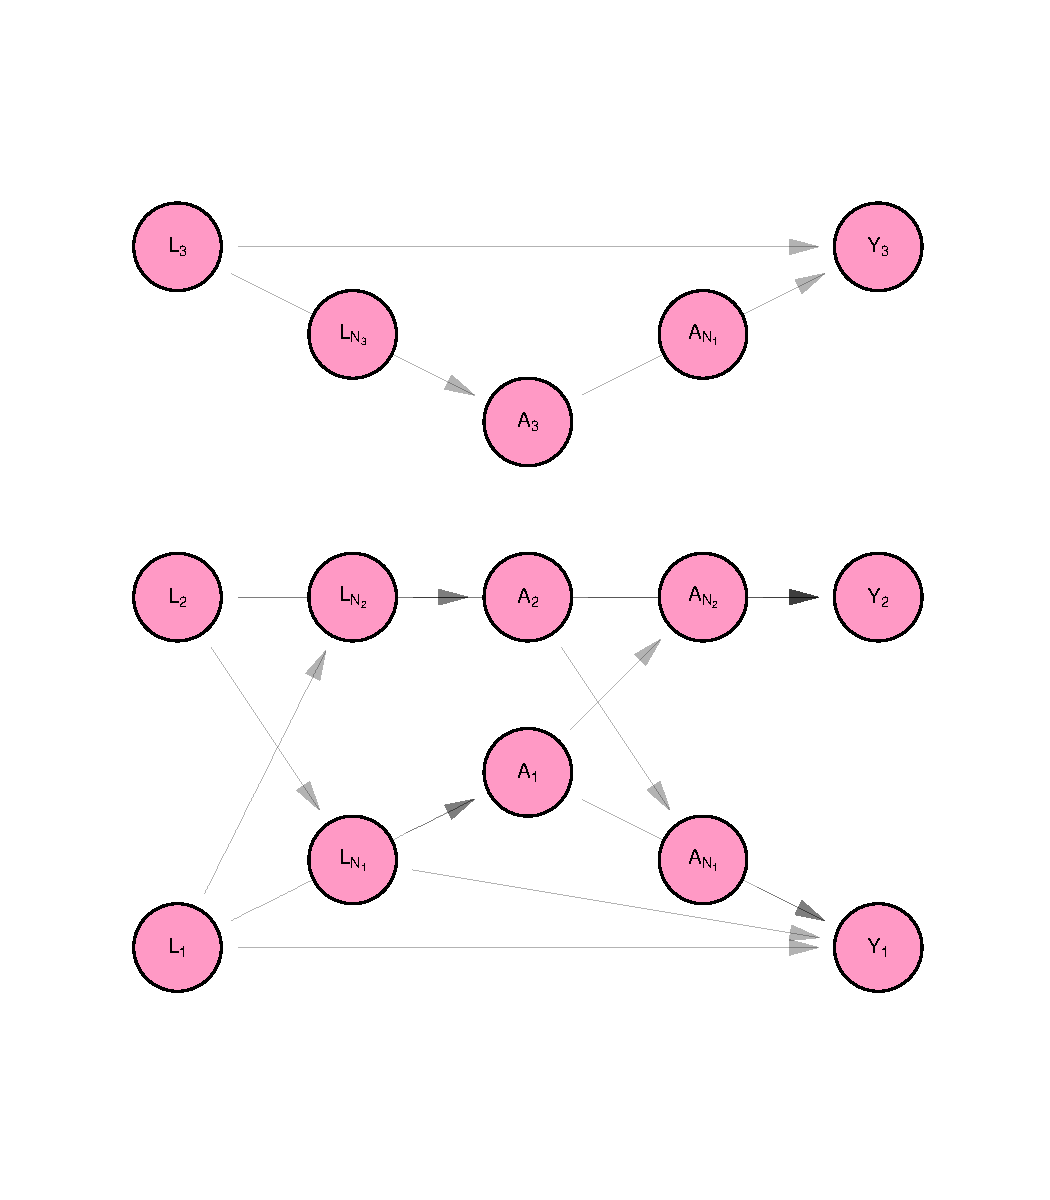
\includegraphics{C_sscan3_causal_interpretation/C__sscan3_causal_interpretation_files/figure-pdf/fig-homogenous-dag-1.pdf}

}

\caption{\label{fig-homogenous-dag}Causal DAG with homogenous structure}

\end{figure}

We can re-write the structural equation model like this:

\begin{equation}\protect\hypertarget{eq-homogenous-dag}{}{
\begin{aligned}
L_i &= f_{L}( U_{L_i} ) \\
A_i &= f_{A}( U_{A_i}, L_i, g_{A}(\textbf{L}_{N_i}) ) \\
Y_i &= f_{Y}( U_{Y_i},  L_i,  g_{Y}(\textbf{L}_{N_i}),   A_i,  h_{Y}( \textbf{A}_{N_i} ) ) \\
\end{aligned}
}\label{eq-homogenous-dag}\end{equation}

\hypertarget{counterfactual-data-1}{%
\subsubsection{Counterfactual data}\label{counterfactual-data-1}}

We define counterfactual outcomes
\(Y_1^{(a_1, \mathbf{a}_{\mathscr{N}_1})}\),
\(Y_2^{(a_2, \mathbf{a}_{\mathscr{N}_2})}\), and
\(Y_3^{(a_3, \mathbf{a}_{\mathscr{N}_3})}\), which represent the level
of job opportunities, \emph{Persons 1}, \emph{2}, and \emph{3}, would
have if we set their dress to level \(a_1\), \(a_2\), and \(a_3\),
respectively. Then the model for counterfactual variable is given by
Equation~\ref{eq-homogenous-interference-swig}. It is represented using
a Single World Intervention Graph (SWIG) in
Figure~\ref{fig-homogenous-interference-swig}.

Note that because of the assumption of network interference, the
counterfactual outcome for \emph{Person 1} is a function of \emph{Person
2}'s treatment value, and vice versa. The counterfactual outcome for
\emph{Person 3}, on the other hand, is a function of \emph{Person 3}'s
treatment (\(a_3\)) alone. This is because \(\mathscr{N}_1 = \{2\}\),
\(\mathscr{N}_2 = \{1\}\), and \(\mathscr{N}_3 = \{\}\), according to
Example 2.

\begin{Shaded}
\begin{Highlighting}[]
\FunctionTok{make\_swig}\NormalTok{(}\StringTok{"homogenous\_interference"}\NormalTok{)      }\SpecialCharTok{|\textgreater{}} 
  \FunctionTok{plot\_swig}\NormalTok{(}\AttributeTok{node\_radius =} \FloatTok{0.2}\NormalTok{) }\SpecialCharTok{+} 
  \FunctionTok{scale\_fill\_mpxnyc}\NormalTok{(}\AttributeTok{option =} \StringTok{"light"}\NormalTok{) }\SpecialCharTok{+}
  \FunctionTok{theme\_mpxnyc\_blank}\NormalTok{()}
\end{Highlighting}
\end{Shaded}

\begin{figure}[H]

{\centering 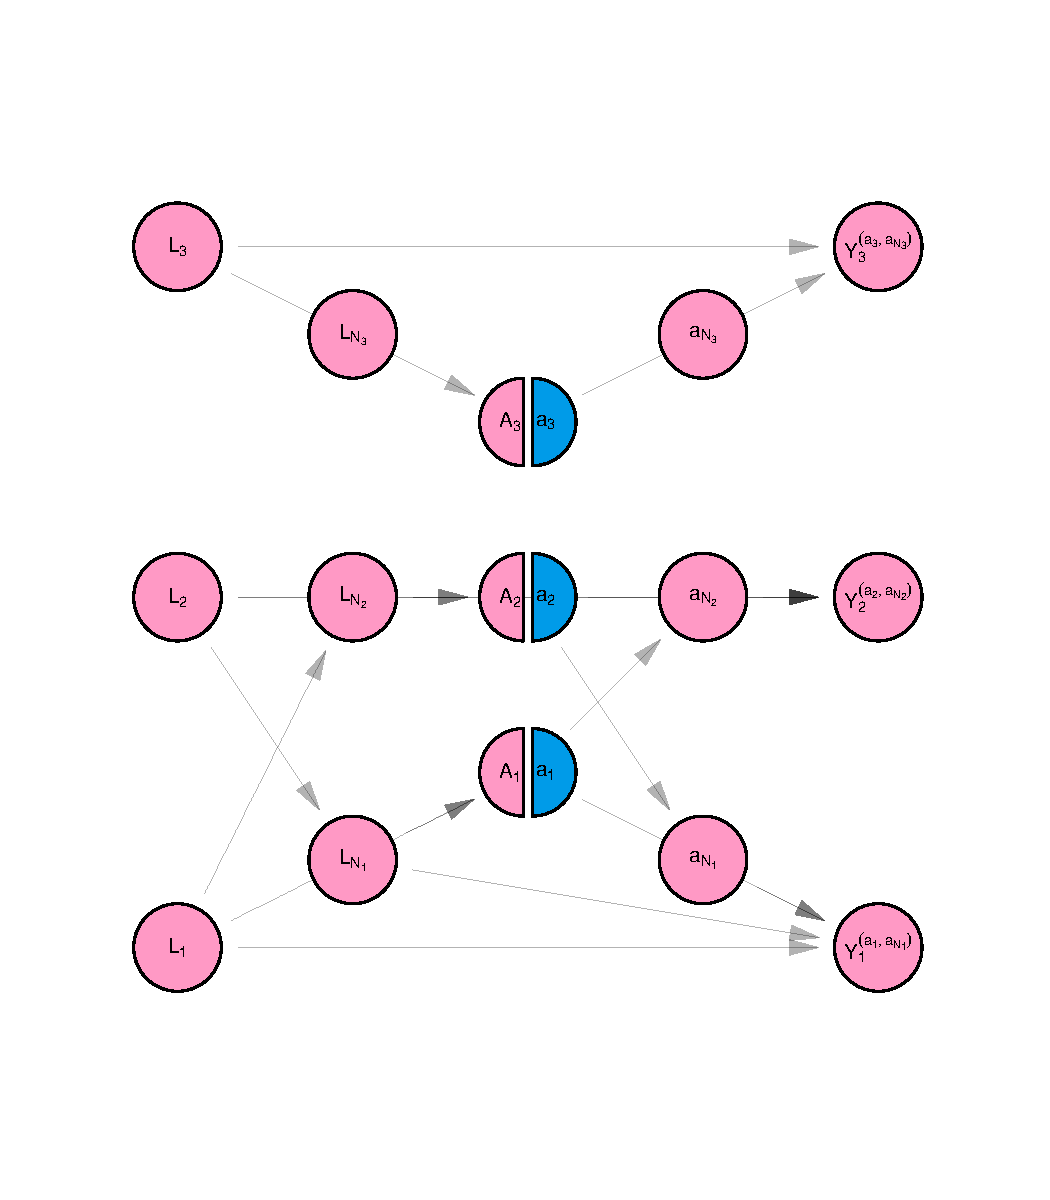
\includegraphics{C_sscan3_causal_interpretation/C__sscan3_causal_interpretation_files/figure-pdf/fig-homogenous-interference-swig-1.pdf}

}

\caption{\label{fig-homogenous-interference-swig}SWIG with network
interference}

\end{figure}

\begin{equation}\protect\hypertarget{eq-homogenous-interference-swig}{}{
\begin{aligned}
L_i &= f_{L}(  U_{L_i}  ) \\
A_i &= f_{A}( U_{A_i}, L_i, g_{A}(\textbf{L}_{\mathscr{N}_i}) ) \\
Y_i^{(a_i,\textbf{a}_{\mathscr{N}_i} )} &= f_{Y}(U_{Y_i}, L_i,  a_i,  g_{Y}(\textbf{L}_{\mathscr{N}_i}),      h_{Y}(\textbf{a}_{\mathscr{N}_i})         ) \\
\end{aligned} 
}\label{eq-homogenous-interference-swig}\end{equation}

\hypertarget{estimates-1}{%
\subsection{Estimates}\label{estimates-1}}

\hypertarget{causal-estimands}{%
\subsubsection{Causal estimands}\label{causal-estimands}}

We are interested in whether on average, in our population of three
people, changing someone's dress would change their level of job offers
To determine the answer, we will compare the average counterfactual
outcome of job opportunities if everyone wore formal dress to the
average counterfactual outcome of job opportunities if everyone wore
non-formal dress. i.e.~We will make the following comparison.

\[ 
\frac{1}{n}\sum_i E[Y_i^{(a = 1, \mathbf{a}_{\mathscr{N}_i} = \textbf{ 1})} - Y_i^{(a = 0, \mathbf{a}_{\mathscr{N}_i} = \textbf{ 0})}]
\]

It is possible to decompose this average causal effect into a portion
attributable to direct (within individual) causal pathways. This tells
us, on average, to what extent one's own dress affects one own's job
opportunities.

\[ 
\frac{1}{n}\sum_i E[Y_i^{(a = 1, \mathbf{a}_{\mathscr{N}_i} = \textbf{ 0})} - Y_i^{(a = 0, \mathbf{a}_{\mathscr{N}_i} = \textbf{ 0})}]
\] We can calculate the portion of the average total effect attributable
to spillover (cross-individual) causal pathways. This tells us, on
average, to what extent one's spouse's dress affects one's job
opportunities.

\[ 
\frac{1}{n}\sum_i E[Y_i^{(a = 1, \mathbf{a}_{\mathscr{N}_i} = \textbf{ 1})} - Y_i^{(a = 1, \mathbf{a}_{\mathscr{N}_i} = \textbf{ 0})}]
\]

\hypertarget{identification-3}{%
\subsubsection{Identification}\label{identification-3}}

\[
\begin{aligned}
E \left[ \frac{1}{n} \sum_i Y_i^{(a_i, \mathbf{a}_{\mathscr{N}_i})}  \right] &= E \left[ \frac{1}{n} \sum_i E[Y_i^{(a_i, \mathbf{a}_{\mathscr{N}_i})}  | \mathbf{L}] \right] \\
\end{aligned}
\] We can start by using the law of iterated expectations. Then we can
evaluate the inner expectation as follows:

\[
\begin{aligned}
 E[Y_i^{(a_i, \mathbf{a}_{\mathscr{N}_i})} | \mathbf{L}]  
        &=  E[Y_i^{(a_i, \mathbf{a}_{\mathscr{N}_i})}   &| L_i , g(\mathbf{L}_{\mathscr{N}_i})] \phantom{, A_i = a_i, h_Y(\textbf{A}_{\mathscr{N}_i}) = h_Y(\textbf{a}_{\mathscr{N}_i})} \\ 
        &=  E[Y_i^{(a_i, \mathbf{a}_{\mathscr{N}_i})}   &| L_i , g(\mathbf{L}_{\mathscr{N}_i}), A_i = a_i, h_Y(\textbf{A}_{\mathscr{N}_i}) = h_Y(\textbf{a}_{\mathscr{N}_i})] \\
        &=   E[f_{Y}(...)                             &| L_i , g(\mathbf{L}_{\mathscr{N}_i}), A_i = a_i, h_Y(\textbf{A}_{\mathscr{N}_i}) = h_Y(\textbf{a}_{\mathscr{N}_i})] \\ 
        &=   E[Y_i                                    &| L_i , g(\mathbf{L}_{\mathscr{N}_i}), A_i = a_i, h_Y(\textbf{A}_{\mathscr{N}_i}) = h_Y(\textbf{a}_{\mathscr{N}_i})] 
\end{aligned}
\]

\begin{itemize}
\item
  In the first line, we use the fact that
  \(Y_i^{(a_i, \mathbf{a}_{\mathscr{N}_i})}\) is independent of \(L_j\)
  for \(j \not \in \mathscr{N}_i\) once we condition for \(L_i\) and
  \(g(\mathbf{L}_{\mathscr{N}_i})\) - the network exposure value for
  person \(i\) with respect to \(\mathbf{L}\).
\item
  In the second line, we use the fact that
  \(Y_i^{(a_i, \mathbf{a}_{\mathscr{N}_i})}\) is independent of
  \(\mathbf{a}\) after adjusting for \(L\), since \(\mathbf{a}\) is a
  constant of the experimenters choosing.
\item
  We replace \(Y_i^{(a_i, \mathbf{a}_{\mathscr{N}_i})}\) with its
  structural equation Figure~\ref{fig-homogenous-interference-swig},
  noting that this is equal to the observed value \(Y_i\) for people
  \(i\) whose treatment value \(A_i\) and network exposure value
  \(h_Y(\textbf{A}_{\mathscr{N}_i})\) is consistent with the value of
  \(\mathbf{a}\) set by the experimenter.
\end{itemize}

We are left with this value

\[
E[ \frac{1}{n} \sum_i  E[Y_i |  L_i , g(\mathbf{L}_{\mathscr{N}_i}), A_i = a_i, h_Y(\textbf{A}_{\mathscr{N}_i}) = h_Y(\textbf{a}_{\mathscr{N}_i}) ]]
\] which we estimate as follows

\[
\frac{\sum_i  E[Y_i |  L_i , g(\mathbf{L}_{\mathscr{N}_i}), A_i = a_i, h_Y(\textbf{A}_{\mathscr{N}_i}) = h_Y(\textbf{a}_{\mathscr{N}_i}) ] I_{\{ x = a\}}(a_i) I_{\{ h_Y (x) = h_Y (\mathbf{a})\}}(a_{\mathscr{N}_i})}{\sum_i I_{\{ x = a\}}(a_i) I_{\{ h_Y (x) = h_Y (\mathbf{a})\}}(a_{\mathscr{N}_i})} 
\]

\hypertarget{reflection-questions-1}{%
\subsection*{Reflection questions}\label{reflection-questions-1}}
\addcontentsline{toc}{subsection}{Reflection questions}

\begin{enumerate}
\def\labelenumi{\arabic{enumi}.}
\item
  Compare and contrast the assumptions made in
  Section~\ref{sec-classic-causal-inference} with those in
  Section~\ref{sec-network-causal-inference}.
\item
  Why might it be useful for network exposure mappings to be bounded
  above? (hint: asymptoptics)?
\item
  Write an example of a network exposure mapping that is not seperable.
\end{enumerate}

\hypertarget{sec-ssnac}{%
\section{SSNAC}\label{sec-ssnac}}

\hypertarget{example-3-longitudinal-data-driven-vaccination-campaign}{%
\subsection*{Example 3: Longitudinal Data-Driven Vaccination
Campaign}\label{example-3-longitudinal-data-driven-vaccination-campaign}}
\addcontentsline{toc}{subsection}{Example 3: Longitudinal Data-Driven
Vaccination Campaign}

You are a public health officer at the department of health in
Nowhereville, and are planning to conduct and assess a three week flu
vaccination campaign. None of the townspeople have been vaccinated
against flu. There is a population of 5 residents in the city, and they
each live in one of three neighborhoods. In addition, residents visit
their friends' homes in other neighborhoods.

\emph{Person 1} lives in \emph{Neighborhood A} and visits
\emph{Neighborhood B}. \emph{Person 2} lives in \emph{Neighborhood B},
but visits \emph{Neighborhoods A} and \emph{B}. \emph{Person 3} lives in
\emph{Neighborhood C} and visits \emph{Neighborhood B}. \emph{Persons 5}
and \emph{6} live in \emph{Neighborhood C} and they do not visit any
other neighborhoods.

The city of Nowhereville has a very structured approach to vaccination
campaigns. At the beginning of each week, each neighborhood gets a risk
rating based on the prevalence of vaccination among its residents and
visitors. Based on that rating, each neighborhood decides whether to
conduct a local vaccination drive or not. Vaccination drives are done in
the same way regardless of neighborhood - visitors and residents are
offered immediate vaccination at a nearby mobile van through a pop-up
message on the local dating app. Not everyone will receive the messages
because some will not open the app during the period of the campaign.
Those who do will have the choice of getting vaccinated or not. Each
person can only get vaccinated once.

\hypertarget{new-tools-from-the-ssnac-framework}{%
\subsection*{New tools from the SSNAC
framework}\label{new-tools-from-the-ssnac-framework}}
\addcontentsline{toc}{subsection}{New tools from the SSNAC framework}

As we see in Figure~\ref{fig-homogenous-dag}, causal DAGs become quickly
visually cluttered, and therefore unwieldy, once we start depicting
causal systems with multiple observational units. If we added a fourth
observational unit to Figure~\ref{fig-homogenous-dag}, it would be
nearly impossible to see which arrow connects which nodes This is an
important limitation because one of the most useful things about causal
DAGs is that they allow the observational epidemiologist to reason
graphically about the structure of confounding and selection.

\hypertarget{introducing-the-causal-directed-acyclic-network-graph-dang}{%
\subsubsection{Introducing the Causal Directed Acyclic Network Graph
(DANG)}\label{introducing-the-causal-directed-acyclic-network-graph-dang}}

We introduce the causal Directed Acyclic Network Graph (causal DANG) - a
simple extension of the DAG that allows for the representation of
complex causal systems. Like the causal DAG, the causal DANG encodes a
non-parametric structural equation model.

\emph{Compact graphic representation}

DANGs encode the structure of the causal process within individuals
separately from the structure of the causal process across individuals.
The former is termed the ``structural part'' of the DANG and the latter
the ``relational part''.

We represent the structural model defined by
Equation~\ref{eq-homogenous-dag} shown in
Figure~\ref{fig-homogenous-dag}. The first aspect (structural part) of
the causal DANG shows the causal structure within individuals. It is a
DAG of vector-valued variables \(\mathbf{L}\), \(\mathbf{A}\), and
\(\mathbf{Y}\) of length equal to the number of people in the sample.
This DAG has standard interpretation under d-separation rules. It gives
the conditional independencies across these vector-valued random
variables. This is an incomplete set of independencies, however, since
some of the entries in \(\mathbf{A}\) are independent of a given entry
in \(\mathbf{L}\), and others are correlated, for instance. The second
part of the causal DANG (relational part) shows which pairs of
individuals have correlated measures with each other. For instance,
below, we see that individuals 1 and 2 are related.

Causal DANGs give us instructions for constructing causal DAGs in the
face of causal interference. For instance, according to the causal DANG
shown in Figure~\ref{fig-causal-dang-instructions}, follow these
instructions to draw the DAG in Figure~\ref{fig-interference-dag}:

\begin{itemize}
\item
  First represent all the entries of \(\mathbf{L}\), \(\mathbf{A}\), and
  \(\mathbf{Y}\).
\item
  Then for each individual \(i\in \{1,2,3\}\), connect \(L_i\) to
  \(A_i\), \(L_i\) to \(Y_i\), and \(A_i\) to \(Y_i\).
\item
  Finally, for the connected pair \(1\sim 2\), connect \(L_1\) to
  \(A_2\) and \(L_2\) to \(A_1\); connect \(L_1\) to \(Y_2\), and
  \(L_2\) to \(Y_1\), and connect \(A_1\) to \(Y_2\) and \(A_2\) to
  \(Y_1\).
\end{itemize}

\begin{Shaded}
\begin{Highlighting}[]
\NormalTok{structural }\OtherTok{\textless{}{-}} \FunctionTok{example\_dang\_1\_structural}\NormalTok{() }\SpecialCharTok{|\textgreater{}}
                    \FunctionTok{plot\_swig}\NormalTok{(}\AttributeTok{node\_radius =} \FloatTok{0.2}\NormalTok{) }\SpecialCharTok{+}
                    \FunctionTok{scale\_fill\_mpxnyc}\NormalTok{(}\AttributeTok{option =} \StringTok{"light"}\NormalTok{) }\SpecialCharTok{+}
                    \FunctionTok{theme\_mpxnyc\_blank}\NormalTok{()}\SpecialCharTok{+}
\NormalTok{                    ggplot2}\SpecialCharTok{::}\FunctionTok{ggtitle}\NormalTok{(}\StringTok{"Structural Part"}\NormalTok{) }

\NormalTok{relational }\OtherTok{\textless{}{-}} \FunctionTok{example\_dang\_1\_relational}\NormalTok{() }\SpecialCharTok{|\textgreater{}}
                    \FunctionTok{plot\_swig}\NormalTok{(}\DecValTok{0}\NormalTok{, }\DecValTok{0}\NormalTok{, }\AttributeTok{node\_radius =} \FloatTok{0.2}\NormalTok{)  }\SpecialCharTok{+}
                    \FunctionTok{scale\_fill\_mpxnyc}\NormalTok{(}\AttributeTok{name =} \StringTok{"Entity type"}\NormalTok{, }\AttributeTok{option =} \StringTok{"light"}\NormalTok{) }\SpecialCharTok{+}
                    \FunctionTok{theme\_mpxnyc\_blank}\NormalTok{() }\SpecialCharTok{+}
\NormalTok{                    ggplot2}\SpecialCharTok{::}\FunctionTok{ggtitle}\NormalTok{(}\StringTok{"Relational Part"}\NormalTok{) }

\NormalTok{cowplot}\SpecialCharTok{::}\FunctionTok{plot\_grid}\NormalTok{(structural, relational, }\AttributeTok{ncol =} \DecValTok{1}\NormalTok{)}
\end{Highlighting}
\end{Shaded}

\begin{figure}[H]

{\centering 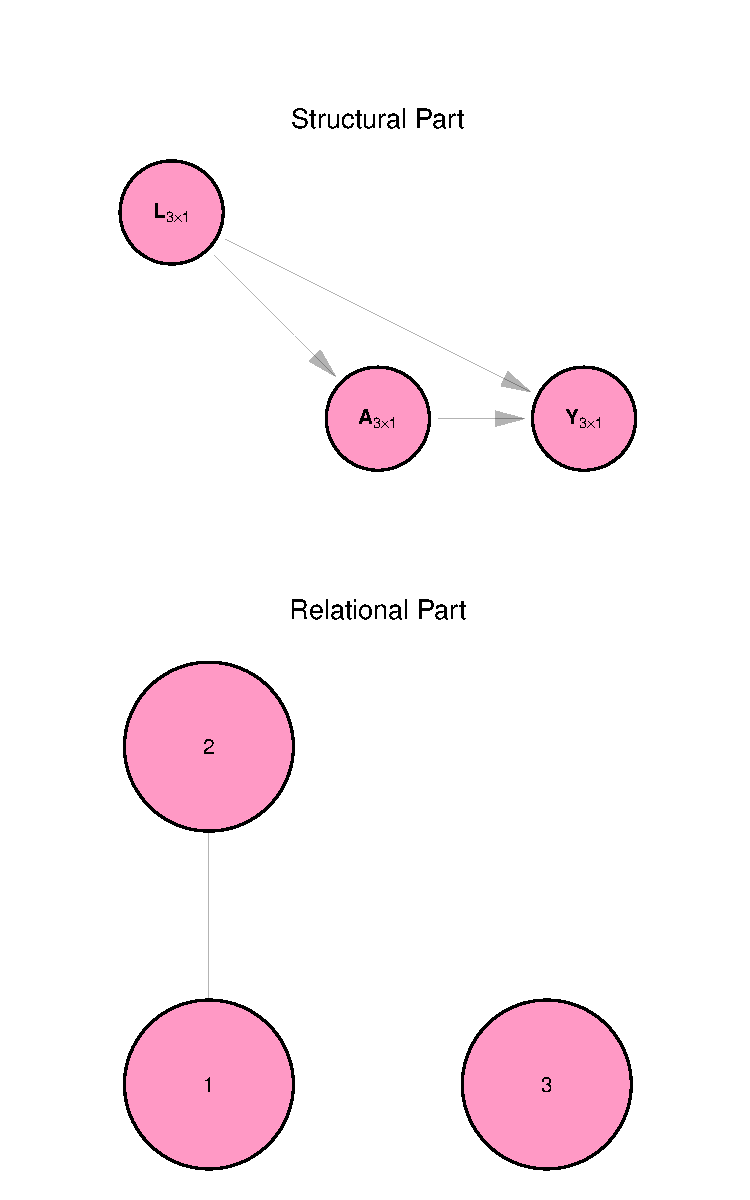
\includegraphics{C_sscan3_causal_interpretation/C__sscan3_causal_interpretation_files/figure-pdf/fig-causal-dang-instructions-1.pdf}

}

\caption{\label{fig-causal-dang-instructions}Causal DANG}

\end{figure}

\emph{Multiple entity types}

The causal DANG relaxes the assumption that all measures in the causal
system can be grouped into non-overlapping sets (i.e.~that each measure
can be attributed to an individual in the sample). In this framework,
different types of entities, represented by vectors of different
lengths, can be depicted on the same DANG.

The causal DANG shown in Figure~\ref{fig-example-dang-structural}
represents the first week of the campaign mentioned in Example 3. Let
\(\mathbf{T}\) be a \(3\times1\) vector whose entries \(T_j\) are 1 if
neighborhood \(j\) is to be vaccinated and \(0\) otherwise.
\(\mathbf{M}\) is a \(5\times1\) vector whose entries \(M_i\) indicate
whether the \(i^{\text{th}}\) person received a vaccination campaign
message or not. \(\mathbf{V}\) is a \(5\times1\) vector whose entries
\(V_i\) show whether participant \(i\) is vaccinated or not.

\begin{Shaded}
\begin{Highlighting}[]
\NormalTok{structural  }\OtherTok{\textless{}{-}} \FunctionTok{example\_dang\_2\_structural}\NormalTok{() }\SpecialCharTok{|\textgreater{}}
                    \FunctionTok{plot\_swig}\NormalTok{(}\AttributeTok{node\_radius =} \FloatTok{0.15}\NormalTok{) }\SpecialCharTok{+}
                    \FunctionTok{scale\_fill\_mpxnyc}\NormalTok{(}\AttributeTok{option =} \StringTok{"light"}\NormalTok{) }\SpecialCharTok{+}
                    \FunctionTok{theme\_mpxnyc\_blank}\NormalTok{() }\SpecialCharTok{+}
\NormalTok{                    ggplot2}\SpecialCharTok{::}\FunctionTok{ggtitle}\NormalTok{(}\StringTok{"Structural Part"}\NormalTok{)}


\NormalTok{relational  }\OtherTok{\textless{}{-}} \FunctionTok{example\_dang\_2\_relational}\NormalTok{() }\SpecialCharTok{|\textgreater{}}
                    \FunctionTok{plot\_swig}\NormalTok{(}\AttributeTok{node\_radius =} \FloatTok{0.2}\NormalTok{, }\AttributeTok{node\_margin =} \DecValTok{0}\NormalTok{)  }\SpecialCharTok{+}
                    \FunctionTok{scale\_fill\_mpxnyc}\NormalTok{(}\AttributeTok{name =} \StringTok{"Entity type"}\NormalTok{, }\AttributeTok{option =} \StringTok{"light"}\NormalTok{) }\SpecialCharTok{+}
                    \FunctionTok{theme\_mpxnyc\_blank}\NormalTok{() }\SpecialCharTok{+}
\NormalTok{                    ggplot2}\SpecialCharTok{::}\FunctionTok{ggtitle}\NormalTok{(}\StringTok{"Relational Part"}\NormalTok{) }

\NormalTok{figure   }\OtherTok{\textless{}{-}}\NormalTok{ cowplot}\SpecialCharTok{::}\FunctionTok{plot\_grid}\NormalTok{(structural, relational, }\AttributeTok{ncol=}\DecValTok{1}\NormalTok{, }\AttributeTok{rel\_heights =} \FunctionTok{c}\NormalTok{(}\DecValTok{3}\NormalTok{,}\DecValTok{3}\NormalTok{))}



\NormalTok{legend\_pre  }\OtherTok{\textless{}{-}}\NormalTok{ relational }\SpecialCharTok{+}\NormalTok{ ggplot2}\SpecialCharTok{::}\FunctionTok{theme}\NormalTok{(}\AttributeTok{legend.position =} \StringTok{"right"}\NormalTok{)}

\NormalTok{legend      }\OtherTok{\textless{}{-}}\NormalTok{ cowplot}\SpecialCharTok{::}\FunctionTok{get\_legend}\NormalTok{(legend\_pre) }
 
   
\NormalTok{cowplot}\SpecialCharTok{::}\FunctionTok{plot\_grid}\NormalTok{(figure, legend, }\AttributeTok{nrow =} \DecValTok{1}\NormalTok{, }\AttributeTok{rel\_widths =} \FunctionTok{c}\NormalTok{(}\DecValTok{4}\NormalTok{,}\DecValTok{1}\NormalTok{))}
\end{Highlighting}
\end{Shaded}

\begin{figure}[H]

{\centering 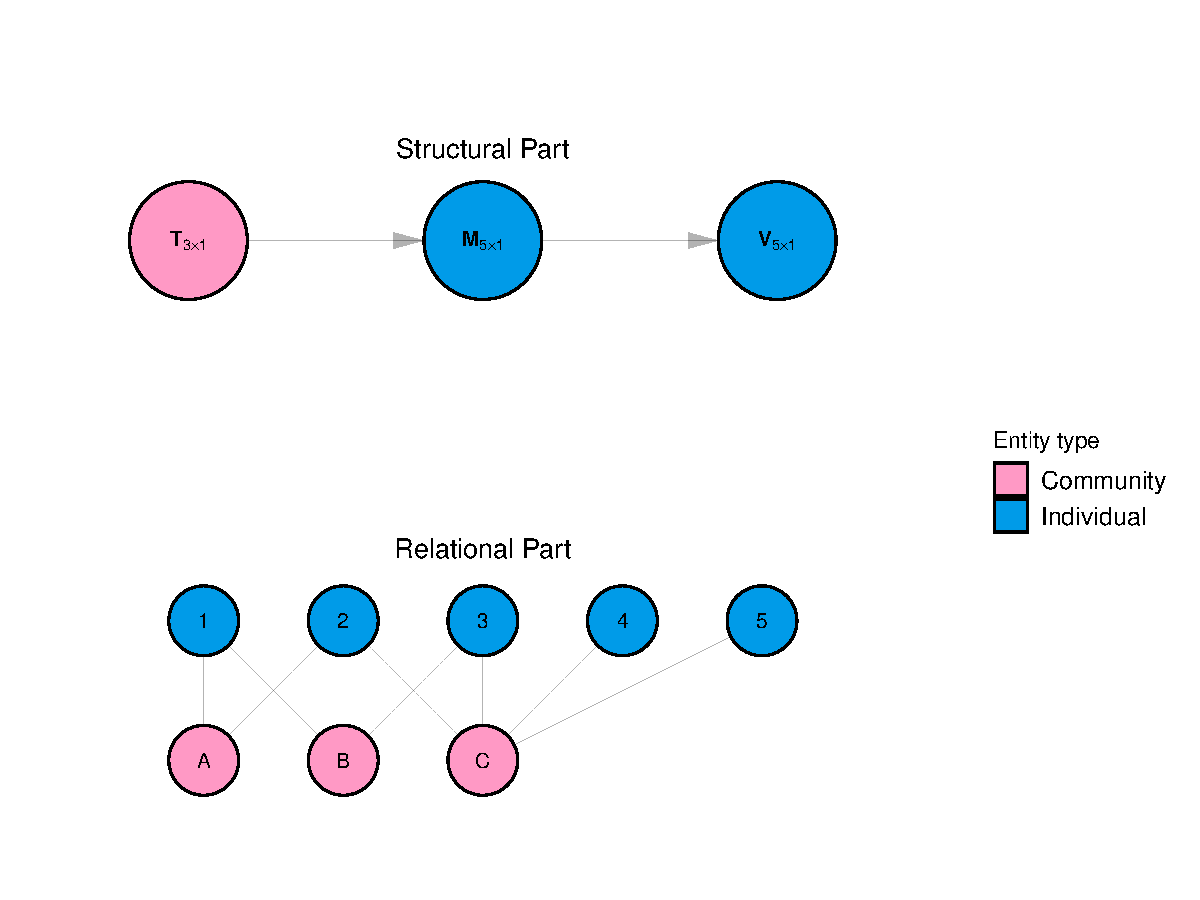
\includegraphics{C_sscan3_causal_interpretation/C__sscan3_causal_interpretation_files/figure-pdf/fig-example-dang-structural-1.pdf}

}

\caption{\label{fig-example-dang-structural}Causal DANG for Week 1 in
Example 3}

\end{figure}

\hypertarget{introducing-the-single-world-intervention-network-graph-swing}{%
\subsubsection{Introducing the Single World Intervention Network Graph
(SWING)}\label{introducing-the-single-world-intervention-network-graph-swing}}

We introduce the Single World Intervention Network Graph (SWING) - a
simple extension of the SWIG that allows for the representation of the
counterfactual outcomes of interventions in complex causal systems.

The SWING has two parts - a structural part and a relational part. Like
the causal DANG, the SWING represents vector-valued random variables
(rather than scalars) as nodes. Like the SWIG, the SWING splits the
nodes that are to be intervened upon by the experimenter.
Figure~\ref{fig-example-swig-structural} shows the counterfactual
distribution of the variables in the model under an intervention setting
\(\mathbf{T}\) to the value \(\mathbf{t}\).

\begin{Shaded}
\begin{Highlighting}[]
\NormalTok{structural  }\OtherTok{\textless{}{-}} \FunctionTok{example\_swing\_structural}\NormalTok{() }\SpecialCharTok{|\textgreater{}}
                    \FunctionTok{plot\_swig}\NormalTok{(}\AttributeTok{node\_radius =} \FloatTok{0.15}\NormalTok{) }\SpecialCharTok{+}
                    \FunctionTok{scale\_fill\_mpxnyc}\NormalTok{(}\AttributeTok{option =} \StringTok{"light"}\NormalTok{) }\SpecialCharTok{+}
                    \FunctionTok{theme\_mpxnyc\_blank}\NormalTok{() }\SpecialCharTok{+}
\NormalTok{                    ggplot2}\SpecialCharTok{::}\FunctionTok{ggtitle}\NormalTok{(}\StringTok{"Structural Part"}\NormalTok{) }


\NormalTok{relational  }\OtherTok{\textless{}{-}} \FunctionTok{example\_swing\_relational}\NormalTok{() }\SpecialCharTok{|\textgreater{}}
                    \FunctionTok{plot\_swig}\NormalTok{(}\AttributeTok{node\_radius =} \FloatTok{0.2}\NormalTok{, }\AttributeTok{node\_margin =} \DecValTok{0}\NormalTok{)  }\SpecialCharTok{+}
                    \FunctionTok{scale\_fill\_mpxnyc}\NormalTok{(}\AttributeTok{name =} \StringTok{"Entity type"}\NormalTok{, }\AttributeTok{option =} \StringTok{"light"}\NormalTok{) }\SpecialCharTok{+}
\NormalTok{                    ggplot2}\SpecialCharTok{::}\FunctionTok{theme}\NormalTok{(}\AttributeTok{legend.position =} \StringTok{"right"}\NormalTok{) }\SpecialCharTok{+}
                    \FunctionTok{theme\_mpxnyc\_blank}\NormalTok{() }\SpecialCharTok{+}
\NormalTok{                    ggplot2}\SpecialCharTok{::}\FunctionTok{ggtitle}\NormalTok{(}\StringTok{"Relational Part"}\NormalTok{)}


\NormalTok{legend\_pre  }\OtherTok{\textless{}{-}}\NormalTok{ relational }\SpecialCharTok{+}
\NormalTok{                    ggplot2}\SpecialCharTok{::}\FunctionTok{theme}\NormalTok{(}\AttributeTok{legend.position =} \StringTok{"right"}\NormalTok{)}
\NormalTok{legend      }\OtherTok{\textless{}{-}}\NormalTok{ cowplot}\SpecialCharTok{::}\FunctionTok{get\_legend}\NormalTok{(legend\_pre) }



\NormalTok{figure   }\OtherTok{\textless{}{-}}\NormalTok{ cowplot}\SpecialCharTok{::}\FunctionTok{plot\_grid}\NormalTok{(structural, relational, }\AttributeTok{ncol=}\DecValTok{1}\NormalTok{, }\AttributeTok{rel\_heights =} \FunctionTok{c}\NormalTok{(}\DecValTok{3}\NormalTok{,}\DecValTok{3}\NormalTok{))}

\NormalTok{cowplot}\SpecialCharTok{::}\FunctionTok{plot\_grid}\NormalTok{(figure, legend, }\AttributeTok{nrow =} \DecValTok{1}\NormalTok{, }\AttributeTok{rel\_widths =} \FunctionTok{c}\NormalTok{(}\DecValTok{4}\NormalTok{,}\DecValTok{1}\NormalTok{))}
\end{Highlighting}
\end{Shaded}

\begin{figure}[H]

{\centering 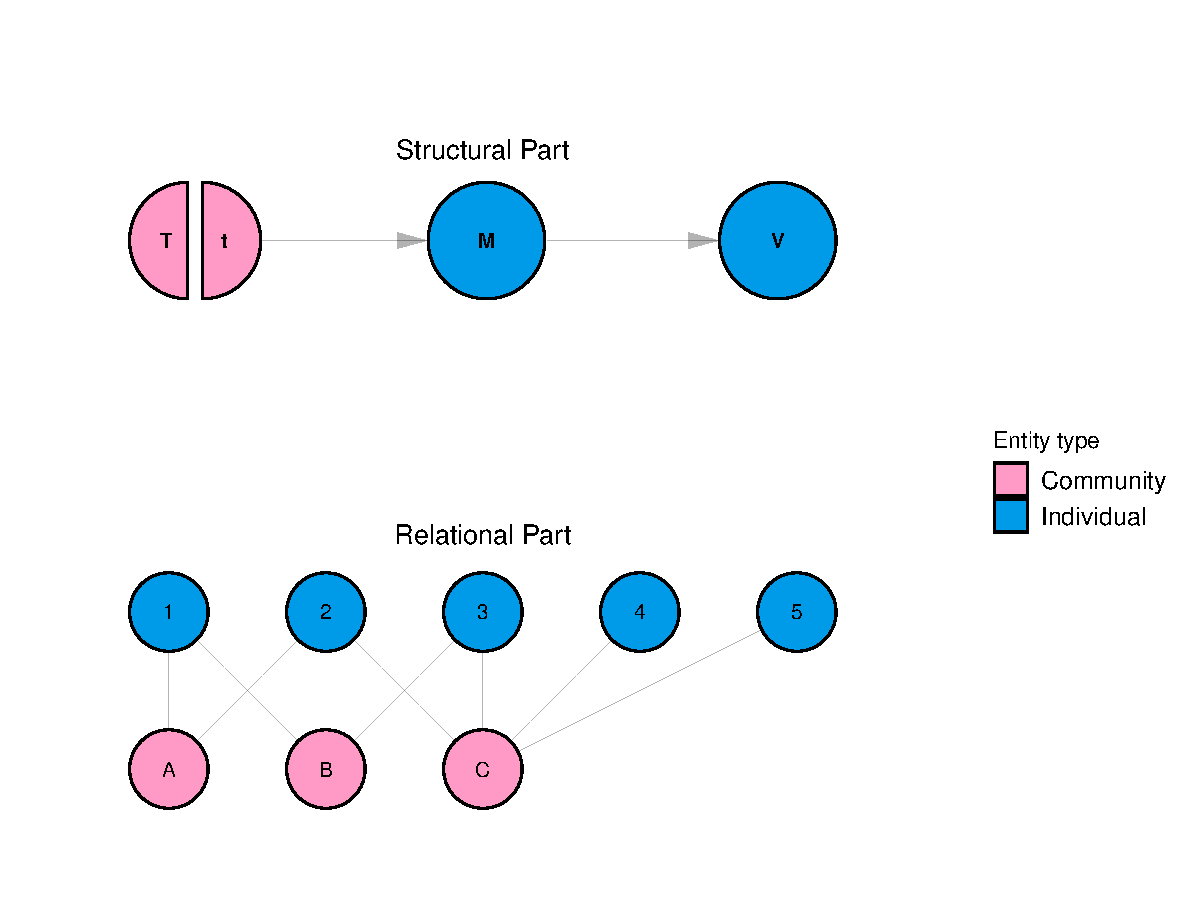
\includegraphics{C_sscan3_causal_interpretation/C__sscan3_causal_interpretation_files/figure-pdf/fig-example-swig-structural-1.pdf}

}

\caption{\label{fig-example-swig-structural}SWING for Week 1 in Example
3}

\end{figure}

\hypertarget{assumptions-1}{%
\subsection{Assumptions}\label{assumptions-1}}

See Section~\ref{sec-network-causal-inference} for a fuller description
of the below assumptions.

\hypertarget{independence-assumptions-1}{%
\subsubsection{Independence
assumptions}\label{independence-assumptions-1}}

Under the SSNAC framework, we make the assumption of \emph{no
spillover}: contemporaneous measurements on observational units of a
given entity type are independent of each other given all prior
measures. The time-ordering of the measurements is given by the
structural part of the causal DANG. We further make the assumption of
\emph{network interference} - that interference respects the mapping
given by the relational part of a causal DANG. i.e.~The exposure mapping
for each equation in the structural equation model is loyal to the graph
that comprises the relational part of the SWING.

\hypertarget{homogeneity-assumptions-1}{%
\subsubsection{Homogeneity
assumptions}\label{homogeneity-assumptions-1}}

We make the \emph{Identical distribution} assumption: the structural
equations that produce each observational unit's measures are identical
across observational units of the same entity type. We assume that the
exposure mapping for each variable in the model is characterized by
\emph{homogeneous interference}. i.e: the exposure mapping is separable,
equivalent, symmetric, and bounded. In applications with repeated
measures, if the structure of the causal DANG allows, the SSNAC
framework allows for the assumption of \emph{time homogeneity}: the
structural equations are identical across time. We apply this assumption
in Example 3 below.

\hypertarget{model-2}{%
\subsection{Model}\label{model-2}}

\hypertarget{observational-data}{%
\subsubsection{Observational data}\label{observational-data}}

The causal DANG shown in Figure~\ref{fig-repeated-observations-dang}
represents the three week campaign mentioned in Example 3 (we omit the
relational part and show only the structural part). Let \(\mathbf{T}_s\)
be a \(3\times1\) vector whose entries \(T_{sj}\) are 1 if
\emph{Neighborhood} \(j\) is to be vaccinated at time \(s\) and \(0\)
otherwise. \(\mathbf{M}_s\) is a \(5\times1\) vector whose entries
\(M_{si}\) indicate whether the \(i^{\text{th}}\) person received a
campaign message at time \(s\) or not. \(\mathbf{V}_s\) is a
\(5\times1\) vector whose entries \(V_{si}\) show whether participant
\(i\) is vaccinated or not at time \(s\). Finally, \(\mathbf{R}_s\) is a
\(3\times1\) vector whose entries \(R_{si}\) shows the risk rating of
neighborhood \(j\) at the beginning of time \(s\).
Equation~\ref{eq-placeintervention-dang} specifies this model for
\emph{Person} \(i\) and \emph{Neighborhood} \(j\) at time \(s\):

\begin{Shaded}
\begin{Highlighting}[]
\FunctionTok{program\_dang}\NormalTok{() }\SpecialCharTok{|\textgreater{}}
  \FunctionTok{plot\_swig}\NormalTok{(}\AttributeTok{node\_radius =} \FloatTok{0.4}\NormalTok{) }\SpecialCharTok{+}
  \FunctionTok{scale\_fill\_mpxnyc}\NormalTok{(}\AttributeTok{option =} \StringTok{"light"}\NormalTok{) }\SpecialCharTok{+}
  \FunctionTok{theme\_mpxnyc\_blank}\NormalTok{()}
\end{Highlighting}
\end{Shaded}

\begin{figure}[H]

{\centering 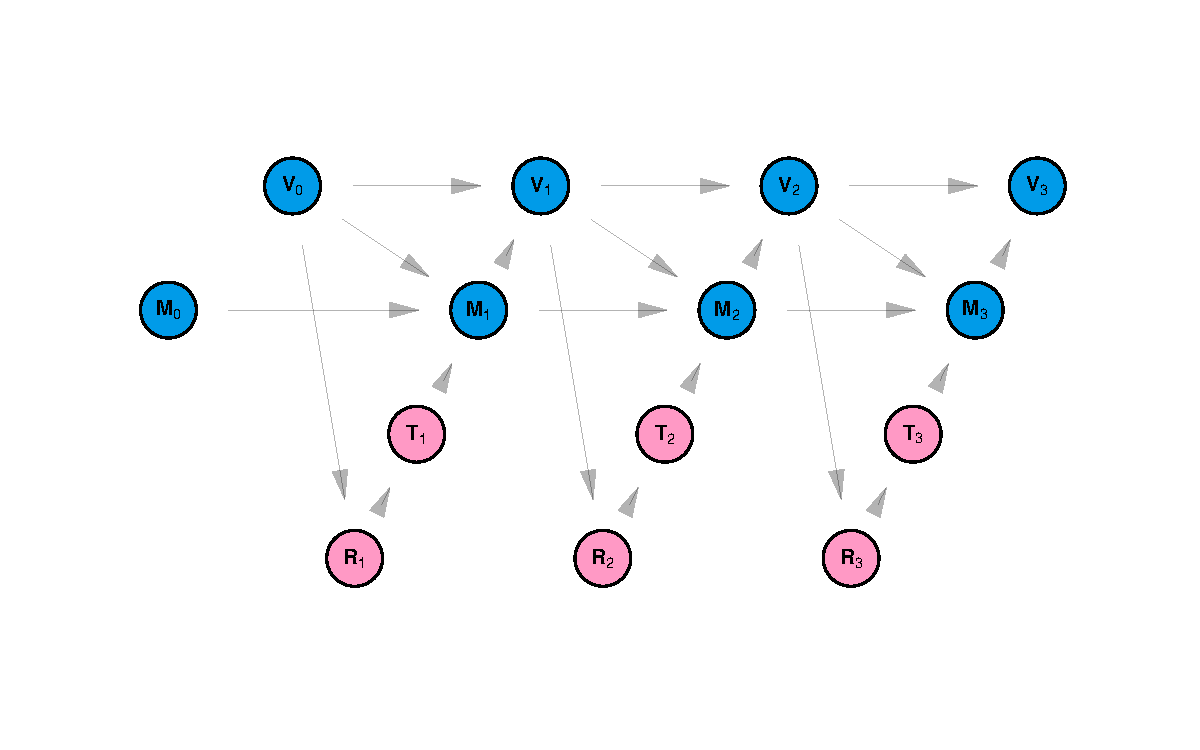
\includegraphics{C_sscan3_causal_interpretation/C__sscan3_causal_interpretation_files/figure-pdf/fig-repeated-observations-dang-1.pdf}

}

\caption{\label{fig-repeated-observations-dang}Causal DANG for Week 1-3
in Example 3}

\end{figure}

\begin{equation}\protect\hypertarget{eq-placeintervention-dang}{}{
\begin{aligned}
M_{0i} &=  f_{M_0}(U_{M_{0i}}) \\
V_{0i} &=  f_{V_0}(U_{V_{0i}}) \\
R_{sj} &=  f_{R}(U_{R_{sj}}, \mathbf{V}_{s-1}) \\
T_{sj} &=  f_{T}(U_{T_{sj}}, R_{s,j}) \\
M_{si} &=  f_{M} (U_{M_{\{si\}}} , V_{\{s-1,i\}}, M_{\{s-1,i\}}, \mathbf{T}_{\{s,\mathscr{N}_i\}})\\
V_{si} &=  f_{V}(U_{V_{\{si\}}}, M_{\{si\}}, V_{\{s-1,i\}}) \\
\end{aligned}
}\label{eq-placeintervention-dang}\end{equation}

According to Equation~\ref{eq-placeintervention-dang}, \(R_{sj}\), the
risk rating for \emph{Neighborhood} \(j\) at time \(s\), is a function
of \(\mathbf{V}_{s-1}\), the vaccination status of every individual at
time \(s-1\). \(T_{sj}\) - an indicator for whether or not
\emph{Neighborhood} \(j\) conducted a campaign at time \(s\), is a
function of the risk rating for \emph{Neighborhood} \(j\) at time \(s\).

\(M_{si}\), which indicates whether or not an \emph{Person} \(i\)
received a campaign message at time \(s\), is a function of whether or
not person \(i\) was vaccinated at time \(s-1\), whether they received a
campaign message at time \(s-1\), and whether or not one of the
neighborhoods they live in or visit conducted a campaign at time \(s\).
The vaccination status of individual \(i\) at time \(s\) is a function
of whether or not they received a campaign message at time \(s\) and
whether or not they were vaccinated at time \(s-1\).

\hypertarget{counterfactual-data-2}{%
\subsubsection{Counterfactual data}\label{counterfactual-data-2}}

Say we want to understand the impact of a vaccination campaign conducted
over three weeks on vaccination status. This would be done by setting
\(\mathbf{T}_1\) to \(\mathbf{t}_1\), \(\mathbf{T}_2\) to
\(\mathbf{t}_2\), and \(\mathbf{T}_3\) to \(\mathbf{t}_3\) and noting
the resulting counterfactual vaccination status at the end of week 1
(\(\mathbf{V}_1^{(\mathbf{t}_1)}\)), week 2
(\(\mathbf{V}_1^{(\mathbf{t}_1, \mathbf{t}_2)}\)), and week 3
(\(\mathbf{V}_1^{(\mathbf{t}_1, \mathbf{t}_2, \mathbf{t}_3)}\)). This
counterfactual model is defined
Equation~\ref{eq-placeintervention-swing} as shown in shown in
Figure~\ref{fig-placeintervention-swing}.

\begin{Shaded}
\begin{Highlighting}[]
\FunctionTok{program\_swing}\NormalTok{() }\SpecialCharTok{|\textgreater{}}
  \FunctionTok{plot\_swig}\NormalTok{(}\AttributeTok{node\_radius =} \FloatTok{0.5}\NormalTok{, }\AttributeTok{nudge\_intervention\_labels =} \FloatTok{0.2}\NormalTok{) }\SpecialCharTok{+}
  \FunctionTok{scale\_fill\_mpxnyc}\NormalTok{(}\AttributeTok{option =} \StringTok{"light"}\NormalTok{) }\SpecialCharTok{+}
  \FunctionTok{theme\_mpxnyc\_blank}\NormalTok{()}
\end{Highlighting}
\end{Shaded}

\begin{figure}[H]

{\centering 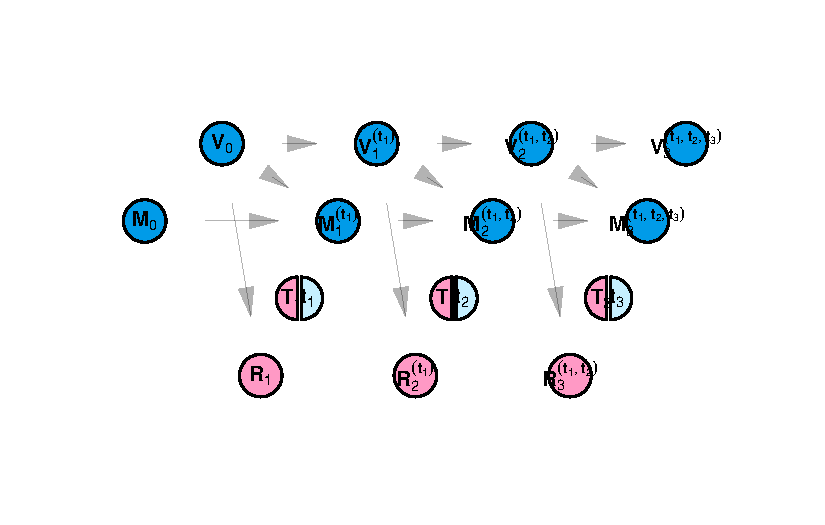
\includegraphics{C_sscan3_causal_interpretation/C__sscan3_causal_interpretation_files/figure-pdf/fig-placeintervention-swing-1.pdf}

}

\caption{\label{fig-placeintervention-swing}SWING for Week 1-3 Example
3}

\end{figure}

\begin{equation}\protect\hypertarget{eq-placeintervention-swing}{}{
\begin{aligned}
M_{0i} &=  f_{M_0}(U_{M_{0i}}) \\
V_{0i} &=  f_{V_0}(U_{V_{0i}}) \\
R_{sj}^{(\bar{\mathbf{t}})} &=  f_{R}(U_{R_{sj}}, \mathbf{V}_{s-1}^{(\bar{\mathbf{t}})}) \\
T_{sj}^{(\bar{\mathbf{t}})} &=  f_{T}(U_{T_{sj}}, R_{s,j}^{(\bar{\mathbf{t}})}) \\
M_{si}^{(\bar{\mathbf{t}})} &=  f_{M} (U_{M_{\{si\}}} , V_{\{s-1,i\}}^{(\bar{\mathbf{t}})}, M_{\{s-1,i\}}^{(\bar{\mathbf{t}})}, \mathbf{t}_{\{s, \mathscr{N}_i\}})\\
V_{si}^{(\bar{\mathbf{t}})} &=  f_{V}(U_{V_{\{si\}}}, M_{\{si\}}^{(\bar{\mathbf{t}})}, V_{\{s-1,i\}}^{(\bar{\mathbf{t}})}) \\
\end{aligned}
}\label{eq-placeintervention-swing}\end{equation}

where \(\bar{\mathbf{t}}\) is defined as ``the history of
\(\mathbf{t}\)''. i.e.~at time 1, \(\bar{\mathbf{t}} =\mathbf{t}_1\). At
time 2, \(\bar{\mathbf{t}} = [\mathbf{t}_1, \mathbf{t}_2]\), etc.

\hypertarget{estimates-2}{%
\subsection{Estimates}\label{estimates-2}}

\hypertarget{causal-estimands-1}{%
\subsubsection{Causal estimands}\label{causal-estimands-1}}

We are interested in vaccine coverage throughout the three week
campaign. For a given week \(s\), this is the sum of the vaccine status
outcome \(\mathbf{V}\) across individuals.

\[
E[\sum_{i=1}^5 V_{si}^{(\bar{\mathbf{t}})}] 
\]

\hypertarget{identification-4}{%
\subsubsection{Identification}\label{identification-4}}

Because individual vaccination status is both a confounder and a
mediator of the relationship between neighborhood intervention status
and vaccination status, we cannot identify our estimands using
conditional expectations of the observed data. We must use a marginal
structural model. See Aronow and Samii (2017).

We can estimate the outcome of interest using the inverse probability of
treatment weights, noting that the treatment in this case is the network
exposure value \(g(t_{\bar{s},N_i})\) for \(\mathbf{T}\).

\[
V_{si}^{(\bar{\mathbf{t}})} =  \frac{V_{si} \mathbf{1}_{x = g(t_{\bar{s},N_i}) }(g(T_{\bar{s},N_i})) }{\prod_{q=1}^s P[g(\mathbf{T}_{q,N_i}) = g(\mathbf{t}_{q,N_i}) | \mathbf{R}_{\bar{q}N_i}]}
\] where \(\mathbf{R}_{\bar{s}N_i}\) is the ``history of
\(\mathbf{R}_{sN_i}\)''. e.g.

\[
\mathbf{R}_{\bar{3}N_i} = [\mathbf{R}_{1N_i}, \mathbf{R}_{2N_i}, \mathbf{R}_{3N_i}]
\]

\hypertarget{reflection-questions-2}{%
\subsection*{Reflection questions}\label{reflection-questions-2}}
\addcontentsline{toc}{subsection}{Reflection questions}

\begin{enumerate}
\def\labelenumi{\arabic{enumi}.}
\item
  Compare and contrast the assumptions made in
  Section~\ref{sec-network-causal-inference} with those made in
  Section~\ref{sec-ssnac}.
\item
  What is the difference between a causal DAG and a causal DANG?
\item
  What is the difference between a SWIG and a SWING?
\end{enumerate}

\hypertarget{sec-control-intervention}{%
\section{Outbreak control intervention}\label{sec-control-intervention}}

We used data from the MPX NYC study to assess the effectiveness of two
approaches to conducting mass vaccination campaigns quickly. MPX NYC is
an online survey of about \(1300\) individuals that was conducted in
2022 in New York City. Study participants were asked to indicate their
home on a map, and were asked to indicate places they had had social
contact in a congregate setting. Spatial coordinates were converted into
community district identifiers. Community districts spatially partition
the city of New York.

\hypertarget{application-outbreak-control-model-using-mpx-nyc-data}{%
\subsection*{Application: Outbreak control model using MPX NYC
data}\label{application-outbreak-control-model-using-mpx-nyc-data}}
\addcontentsline{toc}{subsection}{Application: Outbreak control model
using MPX NYC data}

Under the SSNAC framework, our intervention of interest might not be
about setting the value of any particular variable, but setting a policy
or a process that produces a set of variables in the causal model. This
would be done by changing the structural equations which produce those
variables. In the SWING shown in
Figure~\ref{fig-edge-intervention-swing} and
Equation~\ref{eq-edge-intervention-swing}, we show an intervention which
replaces the function for the risk rating for each community
(\(\mathbf{R}\)) with the function \(h\). Every variable that is
downstream of the first variable created using \(h\) is marked with a
superscript \((h)\) to show that it is partially determined by that
function.

We can now ask what the impact of taking policy \(h\) would be on the
decision whether or not to vaccinate a neighborhood \(j\) at time \(s\)
(\(T_{js}\)). We can also ask what the impact of the policy is on the
the exposure of participant \(i\) to the campaign message at time \(s\)
(\(M_{is}\)).

Our interest in the MPX NYC project, however, was initially to provide
evidence to inform a targeted vaccination campaign, so the main outcomes
of interest are the vaccination status of each individual \(i\) at time
\(s\) (\(V^{(h)}_{is}\)). We were interested in contrasting two
approaches to assigning risk-ratings to community district: the
contact-neutralizing approach, and the movement-neutralizing approach.

Whereas the contact-neutralizing approach ranks community districts by
how many individuals are connected to them, the movement-neutralizing
approach ranks community districts by how centrally they are connected
to other community districts through the mutual connection with certain
individuals.

\hypertarget{assumptions-2}{%
\subsection{Assumptions}\label{assumptions-2}}

We make the simplifying assumption that only one neighborhood is
vaccinated at a time - the top-ranked one. We make the further
simplifying assumptions that every person associated with a community
district (either through residence or social activity) receives the
campaign message when a community district is vaccinated, and that every
person who receives a campaign message gets vaccinated. Once an
individual is vaccinated, they remain vaccinated.

\hypertarget{model-3}{%
\subsection{Model}\label{model-3}}

According to the model specified by structural equations
\ref{eq-edge-intervention-swing}, no individual \(i\) has been
vaccinated at time 0, and nobody receives the campaign message. The risk
rating for community district \(j\) at time \(s\) is some function \(h\)
of the vaccination status at time \(s-1\) for each individual who is
connected to that community district. An intervention is conducted in
community district \(j\) as time \(s\) if that community district has
the highest risk rating. Each individual \(i\) is said to have received
the campaign message at time \(s\) if the intervention was conducted in
any of the community districts he is connected to. Finally, we consider
individual \(i\) vaccinated at time \(s\) if they were vaccinated at
time \(s-1\) or if they received the campaign message in time \(s\). The
risk rating is given by the function \(h\).

\begin{Shaded}
\begin{Highlighting}[]
\FunctionTok{hypothetical\_intervention\_swing}\NormalTok{() }\SpecialCharTok{|\textgreater{}}
  \FunctionTok{plot\_swig}\NormalTok{(}\AttributeTok{node\_radius =} \FloatTok{0.5}\NormalTok{, }\AttributeTok{nudge\_intervention\_labels =} \FloatTok{0.2}\NormalTok{) }\SpecialCharTok{+}
  \FunctionTok{scale\_fill\_mpxnyc}\NormalTok{(}\AttributeTok{option =} \StringTok{"light"}\NormalTok{) }\SpecialCharTok{+}
  \FunctionTok{theme\_mpxnyc\_blank}\NormalTok{()}
\end{Highlighting}
\end{Shaded}

\begin{figure}[H]

{\centering 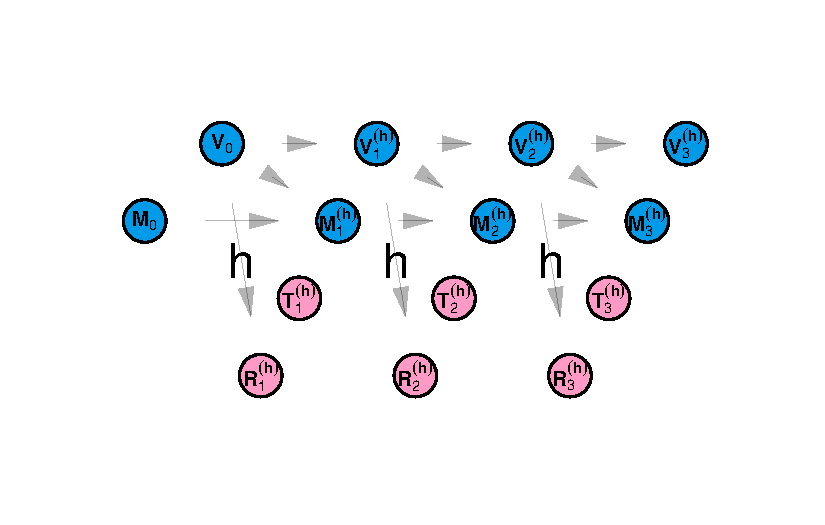
\includegraphics{C_sscan3_causal_interpretation/C__sscan3_causal_interpretation_files/figure-pdf/fig-edge-intervention-swing-1.pdf}

}

\caption{\label{fig-edge-intervention-swing}SWING for Week 1-3 for MPX
NYC Application of SSNAC framework}

\end{figure}

\begin{equation}\protect\hypertarget{eq-edge-intervention-swing}{}{
\begin{aligned}
M_{0i} &=  0 \\
V_{0i} &=  0 \\
R_{sj}^{(h)} &=  h(\mathbf{V}_{s-1}) \\
T_{sj}^{(h)} &=  \begin{cases} 1 & R_{sj}^{(h)} = max_k R_{sk}^{(h)} \\ 0 & \text{otherwise} \end{cases} \\
M_{si}^{(h)} &=  \begin{cases} 1 & \mathbf{T}_{s\mathscr{N}_i}^{(h)} \neq \mathbf{0}  \\ 0 & \text{otherwise} \end{cases} \\
V_{si}^{(h)} &=  \begin{cases} 1 & M_{si}^{(h)} = 1 \text{ or } V_{s-1,i}^{(h)} = 1\\ 0 & \text{otherwise} \end{cases} \\
\end{aligned}
}\label{eq-edge-intervention-swing}\end{equation}

Define \(\psi(i, j)\) as an adjacency function - an indicator function
that equals to \(1\) if Person \(i\) lives in or visits neighborhood
\(j\) and \(0\) otherwise. Let \(\mathscr{N}_P\) be the indices of all
person nodes and \(\mathscr{N}_N\) be a set of indices for neighborhood
nodes. Under the contact-neutralizing approach

\[
h_{sj}(\mathbf{V}_{s-1}) = \sum_{ i \in \mathscr{N}_P} (1 -V_{(s-1), i}) \times \psi(i, j)   
\]

and under the movement-neutralizing approach

\[
h_{sj}(\mathbf{V}_{s-1}) =   \sum_{ i \in \mathscr{N}_P} (1 -V_{(s-1), i}) \times \psi(i, j) \sum_{ k \in \mathscr{N}_N} \psi(i, k) 
\]

\hypertarget{estimands-1}{%
\subsection{Estimands}\label{estimands-1}}

\hypertarget{spatial-efficiency-2}{%
\paragraph{Spatial efficiency}\label{spatial-efficiency-2}}

Intervention coverage for the \(s^{th}\) community district to be
immunized, is defined

\[
C_s^{(h)} = \frac{1}{|\mathscr{N}_p|}\sum_i V_{si}^{(h)} 
\]

The cumulative intervention coverage after immunizing \(s\) community
districts is therefore

\[ 
\bar{C_s}^{(h)} = \sum_{v = 1}^s{C_v }^{(h)}
\]

\hypertarget{social-network-impact}{%
\paragraph{Social network impact}\label{social-network-impact}}

Define graph \(G^{s}(N, \psi_s)\) such that

\[
\psi_s(i, j) = \psi(i, j) \times (1 -V_{(s-1), i})
\]

The cumulative social network impact of immunizing \(s\) community
districts is measured in terms of the size of the largest of the
connected components \(LCC_{(s)}\) of the \(G^{s}(N, \psi_s)\) network
as a proportion of the total number of participants.

\[
\frac{LCC_s}{|N_p|}
\]

\hypertarget{estimation}{%
\subsection{Estimation}\label{estimation}}

We simulated the intervention outlined above using MPX NYC data by
calculating the \(G^{s}(N, \psi_s)\) where \(s\) ranges from \(1\) to
the total number of community districts. We measured the uncertainty of
our estimates by re-sampling study participants with replacement.

\hypertarget{sec-data}{%
\chapter{Survey instrument}\label{sec-data}}

\leavevmode\vadjust pre{\hypertarget{authors}{}}%
Keletso Makofane, PhD

RESPND-MI Collaboration

\hypertarget{mpx-nyc-person-place-network-mapper-1}{%
\section{MPX NYC Person-Place Network
Mapper}\label{mpx-nyc-person-place-network-mapper-1}}

We designed, tested and implemented a survey tool we call the MPX NYC
Person-Place Network Mapper. We named it this because the data collected
through the instrument can be naturally organized into a bipartite
network with nodes representing people and places, and edges
representing relations between people and places. Organizing the data as
a network allows the interpretation of network parameters such as node
degree or connectedness as descriptors of the system connecting people
to each other through the places they traverse within the city.

We designed the tool to solve practical and ethical issues related to
the collection of sensitive spatial data in the context of an annonymous
survey. Practically, we were interested in collecting data on locations
participants visited and possibly had group sex in, but understood that
we would not collect useful data if we collected markers like address or
sip code using usual survey methods. In addition, we had hypothesized
that a sizable proportion of sexual contact in a group happens in
private settings whose addresses and exact locations participants were
likely to forget.

Ethically, we were aimed to collect a data set that would limit the risk
of identifying survey participants through the locations and other data
disclosed through the survey. Collecting spatial coordinates would
increase the risk of accidentally identifying people by, for instance,
capturing the exact coordinate of a college dormitory as a participant's
residence, or capturing the exact coordinates of a federal government
office as a venue for sexual contact in a group setting. In both these
examples, it becomes easier to narrow down the identity of participants
using the location and the particiapnts' characteristics as recorded in
survey data.

\hypertarget{mpx-nyc-person-place-network-map}{%
\subsection{MPX NYC Person-Place Network
Map}\label{mpx-nyc-person-place-network-map}}

Though the investigator team doubted that participants would remember
addresses or zip codes of places they visited, we thought that they
might remember landmarks, cross-streets, neighborhood names, subway
stations names, and other markers New Yorkers use to navigate the city
so we used the Google maps interface and API.

\begin{figure}

{\centering \includegraphics{D_survey_instrument/../_const/images/image_app_graphic.png}

}

\caption{\label{fig-mapinputformat}Map input question format developed
for MPX NYC}

\end{figure}

The MPX NYC Person-Place Network Map question displays a map with
detailed geographic information including place names, roads, and
neighborhood names. It includes a search bar as well as other navigation
tools usually found on a google maps display (see
Figure~\ref{fig-mapinputformat}).

To collect anonymous information on locations, first the participant is
prompted to identify places of a certain type by tapping on the map. For
instance, the first Network Map question asks participants to identify
their primary residence. Once they select one, they are able to move
onto the next question.

The Network Map also allows researchers to elicit a collection of
locations. For instance, we ask participants to identify all the places
they have had physical or sexual contact in a group setting. Each time
the participant taps the map, a marker appears where they tapped, and a
pop-up window asks questions about the most recently identified
location. In our study, participants were asked if they had sexual
contact at the location and to select the type of location it is from a
closed list of options.

\hypertarget{coarsening-to-census-tract}{%
\subsection{Coarsening to census
tract}\label{coarsening-to-census-tract}}

To ensure participant anonymity, the survey tool coarsens spatial data
to the census tract level before sending them to the study database.
Census tracts are non-overlapping spatial units that partition the
United States into areas ranging from \(2500\) to \(8000\) in population
size (US Census 2022). This is done through The Federal Communications
Commission API (FCC 2022) which receives longitude-latitude coordinates
from the survey instrument, and returns census block identifiers, which
are transformed to census tract identifiers by truncating the last X
digits. {[}CITATION{]} It is only after spatial data are transformed
that they are transmitted to the study database (backend).

\hypertarget{development}{%
\subsection{Development}\label{development}}

The front end of the MPX NYC Person-Place Network Mapper was developed
as a single-page web application using the React/NextJS framework
(Vercel 2024) with visual design based on the MPX NYC style guide. The
back end was a custom-built neo4j graph database (Neo4j 2024). Along
with the Network Map question format, the instrument allows the use of
standard survey question formats (multiple choice, single choice, text
field etc.).

\hypertarget{testing}{%
\subsection{Testing}\label{testing}}

The MPC NYC Person-Place Network Mapper underwent two rounds of user
testing. About 10 people participated each time, returning feedback via
an informal feedback questionnaire and via email.

\begin{Shaded}
\begin{Highlighting}[]
\FunctionTok{plot\_icon}\NormalTok{(}\AttributeTok{icon\_name =} \StringTok{"devil"}\NormalTok{, }\AttributeTok{color =} \StringTok{"dark\_orange"}\NormalTok{, }\AttributeTok{shape =} \DecValTok{16}\NormalTok{, }\AttributeTok{alpha =} \FloatTok{0.1}\NormalTok{)}
\end{Highlighting}
\end{Shaded}

\begin{figure}[H]

{\centering 
\includegraphics{D_survey_instrument/D__survey_instrument_files/figure-pdf/unnamed-chunk-2-1.pdf}

}

\end{figure}

\hypertarget{sec-data}{%
\chapter{Study recruitment}\label{sec-data}}

\leavevmode\vadjust pre{\hypertarget{authors}{}}%
Keletso Makofane, PhD

RESPND-MI Collaboration

\hypertarget{mpx-nyc-marketing-and-communication-1}{%
\section{MPX NYC marketing and
communication}\label{mpx-nyc-marketing-and-communication-1}}

\begin{figure}

{\centering \includegraphics{E_marketing_comm/../_const/images/image_campaign_graphic.png}

}

\caption{\label{fig-options}Options for visual identity of MPX NYC''}

\end{figure}

To maximize the speed of recruitment, we invested in a bilingual,
culturally competent communication campaign in collaboration with a
marketing agency. The brief was to create a name and marketing concept
that convey scientific rigor, build trust with the community, and stand
out in a crowded online marketplace (see \textbf{?@fig-requirements}).
As a starting point, the RESPND-MI team suggested a campaign that
playfully uses emojis that have sexual connotations in queer and trans
communities, and that integrates LGBT social media influencers as a
communication channel.

\begin{figure}

{\centering 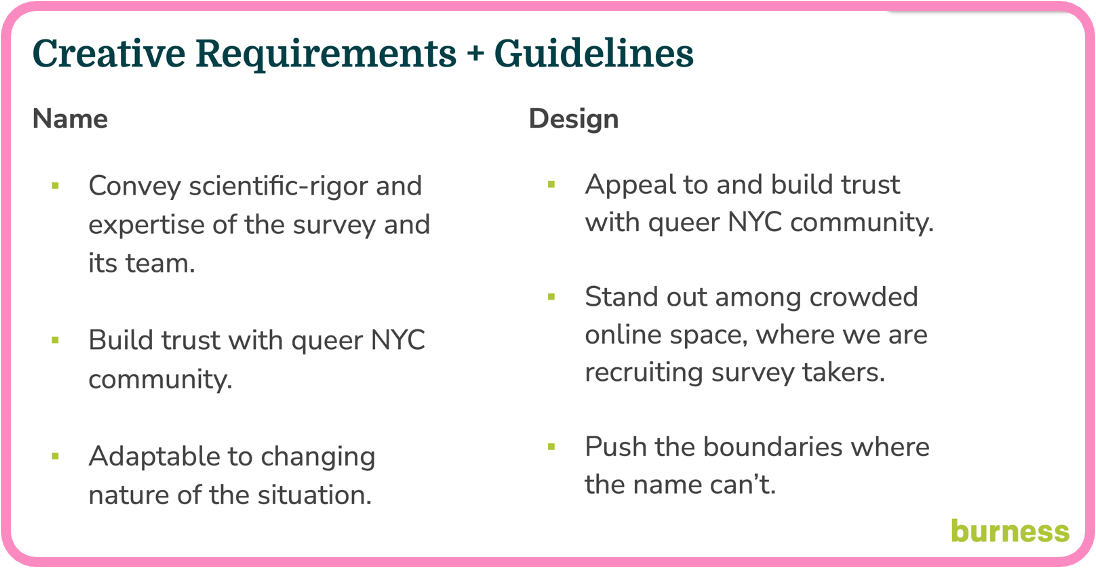
\includegraphics{E_marketing_comm/../_const/images/image_creative_requirements.png}

}

\caption{Requirements for MPX NYC Study}

\end{figure}

Two campaign names and four marketing concepts (see
Figure~\ref{fig-options}) were developed by the marketing agency and
presented to a meeting of the RESPND-MI Community Forum. The final
concept and name were decided by consensus during that meeting.

Marketing materials were developed based on the concept. Materials
included graphics, videos by queer influencers, and a style guide
(including colors, icons, and fonts) for all public-facing materials of
the MPX NYC study. We organized these materials into a ``social media
toolkit'' and shared them through the study website to enable
individuals and organizations to easily share them through their own
social media accounts.

Participants were recruited via paid and donated advertising placed
through Grindr, Twitter, Instagram, and outdoor electronic billboards.

\hypertarget{contracts-and-fundraising}{%
\section{Contracts and fundraising}\label{contracts-and-fundraising}}

Asked for low medium high packaged

Asked for low package to include only intellecgtual work, for medium to
include production, and for high to include advertising spend.

Sequenced fundraising to meet the timing goals.

\begin{Shaded}
\begin{Highlighting}[]
\FunctionTok{plot\_icon}\NormalTok{(}\AttributeTok{icon\_name =} \StringTok{"devil"}\NormalTok{, }\AttributeTok{color =} \StringTok{"dark\_orange"}\NormalTok{, }\AttributeTok{shape =} \DecValTok{16}\NormalTok{, }\AttributeTok{alpha =} \FloatTok{0.1}\NormalTok{)}
\end{Highlighting}
\end{Shaded}

\begin{figure}[H]

{\centering 
\includegraphics{E_marketing_comm/E__marketing_comm_files/figure-pdf/unnamed-chunk-2-1.pdf}

}

\end{figure}

\hypertarget{community-engagement}{%
\chapter{Community engagement}\label{community-engagement}}

\hypertarget{respnd-mi-community-forum}{%
\section{RESPND-MI Community forum}\label{respnd-mi-community-forum}}

Starting in May 2022, we prepared a study about sexual activity and mpox
symptoms among those most vulnerable to mpox. To promote consultation
and collective decision making for the study, we organised an online
community forum (CF). In the first CF, attendees expressed the need for
a space to continually coordinate response efforts across organisations,
and to address gaps not immediately met by local and federal public
health agencies

CFs thus became weekly calls where participants received epidemiologic
updates, discussed problems, and provided input on study design and
marketing decisions. From June to September 2022, over 80 activists,
community leaders, public health professionals participated in CFs. We
produced policy briefs, op-eds, and educational materials; and conducted
media outreach. The RST website became a clearing house for
community-generated resources, as well as community-generated
information on vaccination, testing, and treatment services.

Educational materials and policy recommendations from the CF were
adopted by city, state, and federal PHAs. Reporters cited the RST in
over 90 press clips. Survey data were used to inform NYC vaccination
outreach services. (Roth et al. 2023).

The Community Forum shaped study plans, including the recruitment
campaign, the design of a novel spatial data collection tool, and the
development of our study questionnaire. Sustained engagement led to
several concrete improvements in research approach. For example, a
criticism of the initial communication approach was that it centered
cisgender men to the exclusion of transgender women and transgender men.
This was consistent with most communication about the social
epidemiology of MPOX at the time, and most scientific reporting.

But given that many public heatlh data systems use measures for gender
that are unable to identify transgender individuals, limiting attention
to cisgender men would have limited our ability to understand the true
extent of the mpox outbreak. We assumed that transgender people and
cisgender people are part of the same social and sexual networks which
would likely be affected by mpox. We invited the participant who raised
that criticism to join the study team. Over time, we attempted to
continually improve gender related language and iconography in the
project through discussion among investigators.

\hypertarget{presentations-and-workshops}{%
\section{Presentations and
workshops}\label{presentations-and-workshops}}

Workshops with Martez and Jennifer AIDS Conference Abstracts Academic
talks WHO Talk

\hypertarget{expert-consultations}{%
\section{Expert consultations}\label{expert-consultations}}

People who discussed study design

\hypertarget{project-management}{%
\chapter{Project management}\label{project-management}}

Goals:

\begin{itemize}
\item
  joy, not stress
\item
  low stakes failure
\item
  redundancy
\item
  democracy
\end{itemize}

Approach:

\begin{itemize}
\item
  Elaborate well-structured task list by team
\item
  Assign tasks to indiviuals
\item
  Empower individuals to mark tasks as done or pending
\item
  Empower individuals to re-assign tasks
\item
  Devolve responsibilities, setting clear expectatios
\end{itemize}

Roles:

\begin{itemize}
\item
  Principal investigator

  \begin{itemize}
  \item
    Partnerships
  \item
    Fundraising
  \item
    Drafting study protocol
  \item
    Ethical review of protocol
  \item
    Quality check
  \end{itemize}
\item
  Research coordinator

  \begin{itemize}
  \item
    Schedule group meetings
  \item
    Draft technical documents
  \item
    Research
  \item
    Bookkeeping
  \end{itemize}
\item
  Communications lead

  \begin{itemize}
  \item
    Newsletter
  \item
    Website
  \item
    Attencance lists
  \item
    Press
  \end{itemize}
\item
  Questionnaire lead

  \begin{itemize}
  \item
    coordinate development of questionnaire
  \item
    integrate feedback from stakeholders
  \item
    Seek guidance from technical expertw
  \item
    Work with translation lead
  \end{itemize}
\item
  Web development lead

  \begin{itemize}
  \item
    develop technical specs for web tool
  \item
    Oversee contract with external web developer
  \end{itemize}
\item
  Translation lead

  \begin{itemize}
  \item
    oversee contracts with professional translators
  \item
    quality check translation
  \item
    liase between translator and investigator team
  \end{itemize}
\end{itemize}



\end{document}
